% Plan:
%
% Spis treści
% Spis rysunków
% Słowniczek skrótów
%
% Wstęp (1-2 strony): geneza, obszar, zawartość, dokonania autorów, opis struktury pracy
%
% Rozdziały merytoryczne (4-5, zrównoważone objętościowo):
%   Preambuła (ok. 0.5 strony)
%   Punkty merytoryczne (4-6)
%   Podsumowanie rozdziału
%
%   * opis technologii i uzasadnienie wyboru do rozwiązania problemu
%   * analiza wymagań + projekt systemu (architektura)
%   * opis implementacji, sposób uruchomienia
%   * badania eksperymentalne (tutaj także: profiling, opóźnienia)
%
% Podsumowanie pracy / Zakończenie
%   Wnioski końcowe
%   Co się udało / nie udało (+dlaczego!)
%   Możliwości rozwoju
%
% Spis literatury (numerowany, w tekście _muszą_ być odniesienia, ~20 pozycji)
%
%
% INNE:
%   * całość - ok. 60-70 stron
%   * numeracja - nie więcej, niż 3-poziomowa


\documentclass[11pt]{book}
\usepackage[top=3cm, bottom=4cm]{geometry}
\usepackage[usenames,dvipsnames]{color}


% \usepackage[polish]{babel}
\usepackage[utf8]{inputenc}
\usepackage[T1]{fontenc}
\usepackage{fullpage}
\usepackage[pdfborder={0 0 0}]{hyperref}
\usepackage{float}
\usepackage{graphicx}
\usepackage{scrtime}
\usepackage{tabularx}
\usepackage{listings} 
\usepackage{caption}
\usepackage{color}
\usepackage{hyperref}
\usepackage{tikz}
\usepackage{pgf-umlsd}
% \usepackage[toc,acronym]{glossaries}
\usetikzlibrary{positioning,chains,fit,scopes}

\newcommand{\code}[1]{\begin{tt}{#1}\end{tt}}

\newcommand{\reqlabel}[1]{{\textcolor{Red}{\textbf{#1}}\label{#1}}}
\newcommand{\reqref}[1]{\hyperref[#1]{{\textcolor{Red}{\textbf{#1}}}}}

\newcommand{\tasklabel}[1]{{\textcolor{Blue}{\textbf{#1}}\label{#1}}}
\newcommand{\taskref}[1]{\hyperref[#1]{{\textcolor{Blue}{\textbf{#1}}}}}

% listings settings
\lstset{captionpos=b,frame=single,tabsize=2}

% include TikZ styles
\tikzstyle{terminal}=[
  rectangle,
  minimum size=6mm, rounded corners=3mm,
  very thick,
  draw=black!50,
  top color=white,bottom color=black!20,
  font=\ttfamily
]




\title{Component-based system for management of multilevel virtualization of networking resources}
\author{Robert Boczek \and Dawid Ciepliński}

\begin{document}

  \maketitle
    
  \tableofcontents

  \listoffigures

  \newpage
	\begin{center}
	\vspace*{2in}
	{\it We would like to acknowledge the support and assistance given us by professor Krzysztof Zieliński and Marcin Jarząb. Their generously contributed ideas, 
		feedback and advice was of great help to us.}
	\\
	{\it Finally, we would like to thank to our parents,  for their support and encouragement.}
  \end{center}

  \newpage
	\begin{center}
	\vspace*{2in}
	{\it Thesis work contribution:}\\
	
	{\it Chapters written together ( 2, 4, 8 ), } \\
	{\it Chapters written by Dawid ( 5, 7 ) ,} \\
	{\it Chapters written by Robert ( 1, 3, 6 ), } \\
	{\it Implementation work performed together. }
  \end{center}

  \chapter{Introduction}

    % QoS, rezerwacja zasobów, izolacja we współczesnych systemach informatycznych	
	
	In today's world every successful organisation is based on properly designed communication network. These networks
	must deal with delay-sensitive data such as video images, real-time voice or mission-critical data. Therefore
	must provide safe, predicatable and sometimes guaranteed services. Accomplishing the required Quality of 
	Sevice ( QoS ) by controlling the delay, delay variation(jitter), bandwidth and packet loss parameters is deeply 
	hidden secret of most successful end-to-end business applications. Technologies like Ethernet did not foresee future 
	necessity of providing supporting QoS therefore implementing QoS solutions over the Internet is such a demanding issue. 
	%http://www.cisco.com/en/US/products/ps6558/products\_ios\_technology\_home.html
	
	Increasing popularity of virtualization, isolation and resource reservation in contemporary systems encourages to 
	further reseach. Computing models like \textbf{Cloud computing}, \textbf{Grid computing} are becoming a standard and it 
	is definately worth knowing at least the basic concepts.
	
	%TODO dopisac o rezerwacji zasobow i izolacji
	\medskip
	
	Due to raising concern and importance of these issues this paper takes more insight into one of 
	possible approaches	to those matters which is Solaris OS and the Crossbow technology. In this study, system supporting 
	multilevel virtualization of networking resources with isolated network and QoS elements is taken into consideration.


  \chapter{Context}  % TODO ładniej

    Constantly growing demand for bandwidth in networks (especially VoD, VoIP, RT) raises the question: 'Whether it is
    better to increase available bandwidth of networks or to build intelligent systems managing users traffic?'.  As
    high bandwidth is just not enough because there are other equally important transmission parameters (delay, jitter,
    package missing	tolerance) there seems to be just one correct answer for this question. Creating such systems is not
    an easy task and many groups such as IETF (The Internet Engineering Task Force) are working on this problem.
    Currently there are three existing models performing QoS in the IP network:

    \begin{enumerate}
      \item best effort,
      \item Intserv,
      \item Diffserv.
    \end{enumerate}

    These models are discussed in more details in the following section.


    \section{QoS-aware networking}

      % TODO  krotki przeglad QoS w roznych sieciach, nie tylko IP, ale tez ATM, Frame Relay, Token Ring (na podst.
      % wykl. Luke-a?)
      %
      % w szczegolach o QoS na IP

      QoS (Quality of Service) is an issue in all types of networks such as IP, Token Ring, Frame Relay or even ATM.
      Each of them adapted specific approach towards this matter. IP network for instance is non-deterministic although
      there is a possiblity of packet classification using CoS (Class of Service) field. Token Ring on the other hand is
      deterministic and allows using priority to distinct traffic. Last but not least ATM creates virtual path between
      sender and receiver and sets QoS parameters. Despite the fact that all approaches are very interesting and
      meaningful this paper focuses mainly on the IP network and its approach to QoS.

      % IntServ, DiffServ, inne

      Nowadays the IETF (The Internet Engineering Task Force) is working on two approaches beyond the basic best-effort
      service to provide more advanced handling of packets and providing requested level of bandwidth and delay which
      are:

      \begin{enumerate}
        \item integrated services --- reserves resources necessary to provide the service along path,
        \item differentiated services --- do not require resource reservation along path
      \end{enumerate}


      \subsection{DiffServ}

        Due to clear need for relatively simple and coarse methods of providing differentiated classes of service for
        Internet traffic, to support various types of applications, and specific business requirements. The
        differentiated service approach to providing quality of service in networks employs a small, well-defined set of
        building blocks from which a variety of aggregate behaviors may be built. \cite{qos}

        DiffServ works with traffic stream containing many complex microflows which among the same stream have:

        \begin{itemize}
          \item Same QoS requirements,
          \item Traverses domain towards the same direction.
        \end{itemize}

        Microflow is a flow between applications and is identified mainly by:

        \begin{enumerate}
          \item Source and/or Destination Address,
          \item Transport protocol,
          \item Source and/or Destination Port.
        \end{enumerate}

        \begin{figure}[H]
          \begin{center}
            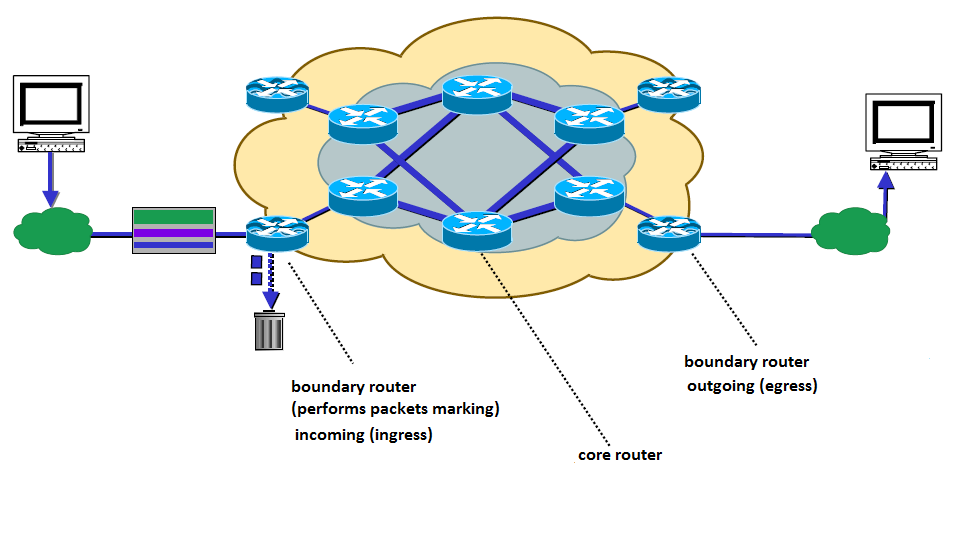
\includegraphics[width=.7\textwidth]{img/qos/diffserv.png}
          \end{center}
          \caption{DiffServ domain}
        \end{figure} %TODO podac zrodlo obrazka ( wyklad z systemow multimedialnych dotyczacy QoS )

        DiffServ domain is a set of nodes with consistent QoS policy (for example network managed by the same ISP or
        intranet). Routers within domain are didvided into two groups: boundary routers and core routers. Boundary
        router performs traffic classification, packet marking, traffic metering, traffic control (policing, shaping)
        where core routers pass packets according to PHB(Per Hop Behaviour - more about them later) and sometimes
        changes DSCP labels.

        This architecture distinguishes two major components: packet marking using the IPv4 ToS byte or TC in IPv6 and
        PHBs(Per Hop Behaviour).

        \medskip

        Redefined ToS field now uses 6 bits for packet classification and is called Differentiated Services
        Codepoint(DSCP). PHB defines how packet should be treated due to its priority. Accepted policy should be
        consistent within all domain.


      \subsection{IntServ}

        Integrated services beyond the basic best-effort service defined in two RFCs provide two levels of service for
        IP which are called Controlled-Load Service and Guaranteed Service. Both require information about the traffic
        to be generated. 

        Guaranteed Service type should be used in applications with real time demands as it provides guaranteed
        bandwidth and delay, whereas Controlled-Load Service does not give full guarantee and should be used with
        application less sensitive for packets loss or delay.

        IntServ requires resource reservation for certain flows or aggregated data streams. The reservation operation is
        available thanks to RSVP protocol. Due to this reservation session initialization lasts much longer than in
        DiffServ.

        {DiffServ vs IntServ}

        \begin{table}[ht]
          \caption{DiffServ, IntServ comparison}
          \centering % used for centering table
          \begin{tabular}{c c}
            \hline \hline
            IntServ         & DiffServ \\
            Stateful        & Stateless \\
            Not scalable    & Scalable \\
            Stream oriented & Processing single packets \\
            \hline
          \end{tabular}
        \end{table}


    \section{Resource virtualization approaches}

      % TODO classify and define virtualization types


    \section{Multilevel network virtualization}

      The problem of networking resources virtualization is multifaceted. There are many aspects at various levels that
      may be considered --- virtualization at the Data Link Layer of the OSI/ISO model with VLAN technology, providing
      software equivalents of equipment used by higher network layers (e.g. virtual routers), or creating fully virtual
      networks with Quality of Service guarantees. The section provides an in-depth description of these techniques
      together with examples of technologies used.


      \subsection{Virtual network resources}

        % implementacje software-owe: router, firewall
        % warstwa lacza danych: VLANy
        % VPNy?


      \subsection{Fine-grained QoS control}

        % logiczne kanaly/flowy


      \subsection{Virtual appliances}

        % ogolnie o podejsciu, przyklady


      \subsection{,,Network in a box'' concept}

        % cala siec skonsolidowana w jednej maszynie, (zalety, wady,)? przyklady


    \section{Applications and benefits of virtual infrastructures}

      \subsection{Testing and simulations}

      \subsection{Improving server-side infrastructure scalability}

      \subsection{Infrastructure as a service}

        The IAAS (Infrastructure as a service) sometimes also called Hardware as a Service (HaaS) is one of three cloud
        computing models, the other two are: Software as a Service (SaaS) and Platform as a Service (PaaS).  This
        service is based on providing by the supplier whole scalable IT infrastructure depending on user demand such as
        virtualized hardware. The service provider owns the equipment and is responsible for housing, running and
        maintaining it.

        At the beginning the IaaS was just renting dedicated servers services from supplier. Nowadays thanks to
        virtualization these are most often virtual machines. In the former case user paid for the concrete hardware
        (box), now client typically pays on a per-use basis.


      \subsection{The role of resource virtualization in the SOA stack}


    \section*{Summary}


  \chapter{Requirements analysis}

    This chapter focuses mainly on earlier conducted requirements analysis and extracted conclusions. Established goal
    was to create system supporting creation of any requested, fully isolated network structure with virtual network
    elements and demanded resources recovered from selected (previously prepared) repository and fully monitored network
    traffic. This target implicated necessity of creating functional and non-functional specification in order to avoid
    ambiguities and skipping essential services. All these issues are described and considered in the first two
    chapters.

    Section \ref{sec:req:func} presents requested behaviors (functions or services) of the system that support user
    goals, tasks or activities.

    Section \ref{sec:req:nonfunc} describes adopted non-functional requirements towards newly created system.


    \section{Functional requirements}
	
		\label{sec:req:func}
		
		All services of the system have been divided into three groups: accounting, discovery and instantiation.
                These division have been performed based on the quality of the functionality.  

      \subsection{Instantiation}
		\label{sec:req:func:inst}
	  
		Most of functionalities neccessary during process of network instantiation ( also alteration and \\ deletion ) would be:
		
		\begin{itemize}
			\item{Creation of any requested virtual network element, }
			\item{Creation of any requested resource from repository, }
			\item{Assignation any number of links to resource, }
			\item{Resource routing table modification, }
			\item{Defining QoS limits to links and flows ( limits traffic assigned to specific network traffic \\ type ), }
			\item{Modification or deletion of each property and element previously mentioned. }
		\end{itemize}
		

      \subsection{Discovery}
		\label{sec:req:func:disc}
		
		During the process of discovery following functionalities should be accessible:
		
		\begin{itemize}
			\item{Discovery and assembly of links, resources from the same project, }
			\item{Detection of links assigned to a specified resource, }
			\item{Discovery of flows attached to a link. }
		\end{itemize}


      \subsection{Accounting}  % kz: raczej Monitoring
		\label{sec:req:func:acc}
		
		In terms of accounting, following functionalities for properties and elements should be provided:
		
		\begin{itemize}
			\item{Monitoring of each link's bandwidth, }
			\item{Checking each link's, flow's network traffic ( input / output ) statistics, }
			\item{Displaying network traffic load chart of selected link or flow from specified time period. }
		\end{itemize}

    \section{Non-functional requirements}
		\label{sec:req:nonfunc}

    % TODO model obiektowy jak najbardziej niezalezny od systemu pod spodem
	
		Non-functional requirements also called \textbf{qualities} of a system could be distincted between 
		the executing system and the work products ( created during system development ). Executing system are related
		to user goals and are refered as run-time qualities, whereas work products are driven by the development organization’s
		goals and refered as development-time qualities \cite{nonfunctional}. 

                \medskip
		
		Requested run-time qualities:
		\begin{itemize}
			\item{usability - usage should be intuitive, system should be efficient,}
			\item{operational scalability - system should support additional users or sites, }
			\item{configurability - configurable properties should be easy to set,}
			\item{adaptable - ability to adapt to changing conditions ( adding removing new nodes ),}
			\item{fault tolerance - system should be resistant for minor erros.}
		\end{itemize}
		
		\medskip
		
		Requested development-time qualities:
		\begin{itemize}
			\item{independent and reusable object model - created model should be general without system specific details, }
			\item{evolvability - support for new functionalities or adjustement to new technologies,}
			\item{extensibility - ability to add new earlier unspecified functionalities, }
			\item{composability - system should be created in form of composable components, }
			\item{reusability - ability to (re)use in future systems.}
		\end{itemize}
		

    \section{Underlying environment characteristics}
	
		Underlying environment should be a composition of a fully independent nodes. However, a few requisites
		must be fulfilled by each node:
		
		\begin{itemize}
			\item{Each OS should have the crossbow functionality provided, }
			\item{Network accessibility between nodes must be ensured. }
		\end{itemize}
		
	%TODO ta czesc tak srednio mi tu pasuje!!!

    \section{General approach and problems it imposes}
	
		Selected approach towards problem was 

      \subsection{Load balancing / Deployment}
	  
		Although at first load balancing was planned, created system does not support it. This matter is further 
		discussed in \textbf{'Further work'} section in the \textbf{Summary} chapter.
		
		In terms of deployment, potential problems are easy to indicate. Use of Jims functionality and related JMX 
		features stresses the lack of transactional support. Although in our system in case of errors introduced changes
		are usually removed, there is no guarantee that it will acutally happen. Due to possible further errors caused during 
		restoring previous system state. In that case these partial changes must be removed manually from each node
		involved in this failing deployment attempt which generally imposes specialistic knowledge of underlying environment. 

      \subsection{Infrastructure isolation}
	  
		Network isolation is provided thanks to the Crossbow functionality which is more accuratly described in the chapter
		about Solaris OS features. 
		
		%TODO what about resource isolation CPU/MEM ? 
    % TODO izolacja podczas wykorzystywania wielu maszyn polaczonych kablem

      \subsection{Broadcast domain preservation}

        % TODO o vlanach
	  
		

      \subsection{Constraints}


  \chapter{Solaris 10, Solaris 11 and OpenSolaris}
  
    %TODO change chapter title !!! // Solaris OS as a resource virtualization environment
    % TODO  actually, Solaris 10, Solaris 11 and OpenSolaris are described here!

    The chapter provides an overview of Oracle Solaris operating system and evaluates it as a platform for resource
    virtualization. The chapter describes Solaris 11 Express release of the system, as it is the first release
    (together with OpenSolaris) with Crossbow technology integrated. Special emphasis is put on the networking-related
    aspects of virtualization. Thus, the Solaris Crossbow technology is described in detail.

    Section \ref{sec:sol:general} contains introductory information about the system. A short historical note is
    presented and general description follows. Main components of the system are introduced and described.
    
    Each of the remaining sections describe in more detail these parts of the operating system that are extensively
    used by the implemented system. Section \ref{sec:sol:containers} investigates the Solaris Zones technology. After
    defining the concept of zones, zone lifecycle model is presented, the achieved level of process isolation is
    described and discussion of Zones advantages in comparison to non-virtualized environments follows.

    Section \ref{sec:sol:xbow} introduces Solaris Crossbow - lightweight network virtualization environment. The
    section starts with general description of the technology. Next, components crucial to efficiency improvement are
    presented in detail. Etherstubs, VNICs and flows are described. These are building blocks used to create
    virtualized network elements and apply QoS policies. The section ends with the comparison between Crossbow and
    DiffServ and a method of integration of these two solutions is presented.

    Section \ref{sec:sol:res} provides an overview of resource control methods offered by the Solaris OS. The types
    of resource management mechanisms (constraints, partitioning and scheduling) are identified and defined. Resource
    control hierarchy used by the system is depicted and explained. Also, the accounting facility is described. The
    types of resources extended accounting can work with are enumerated and examples of data that can be gathered are
    listed.


    \section{General information}
    \label{sec:sol:general}

      Oracle Solaris is a \textit{multiuser, multitasking, multithreading UNIX-like operating system} \cite{reference}.
      Since its release in 1992 (as Sun Solaris 1), the system became one of the most popular environments supporting
      enterprise software. Nowadays, big corporations and companies as well as individual developers use it to do their
      business and deliver reliable and scalable services.

      The Solaris OS provides unique set of tools that support virtualization of practically all types of resources at
      various levels. There is Logical Domains (LDOMs) technology for full virtualization and lightweight Zones, when
      all that is needed is the isolation of processes. Logical domains can be connected with complex virtual networks
      that are created with virtual switches (vsw) and virtual network devices (vnet) \cite{ldomag} and Crossbow can be
      used to enable lightweight and efficient networking for zones, exploiting capabilities of underlying hardware
      layer (network interface cards with virtualization level 1, 2 or 3 \cite{santos}).

      Resource utilization can be managed with integrated administration tools. Resource access policies can be created
      with high level of granularity (per-process resource control) as well as in more general way (limiting resource
      access for LDOMs). Resource consumption can be subject of monitoring and accounting. With extended accounting
      subsystem enabled, it is possible to capture detailed accounting data even for single processes. Gathered data
      include CPU usage, number of bytes received or transmitted per DiffServ or Crossbow flow and more.

      As far as multiple physical machines are considered, there is also support for VLANs (Virtual Local Area Network).
      Thanks to VLAN tagging support, it is possible to build systems that guarantee the quality of service from the
      lowest levels up, even for services belonging to different systems and consolidated within single physical machine.

      \begin{figure}[H]
        % TODO expand
        \begin{center}
          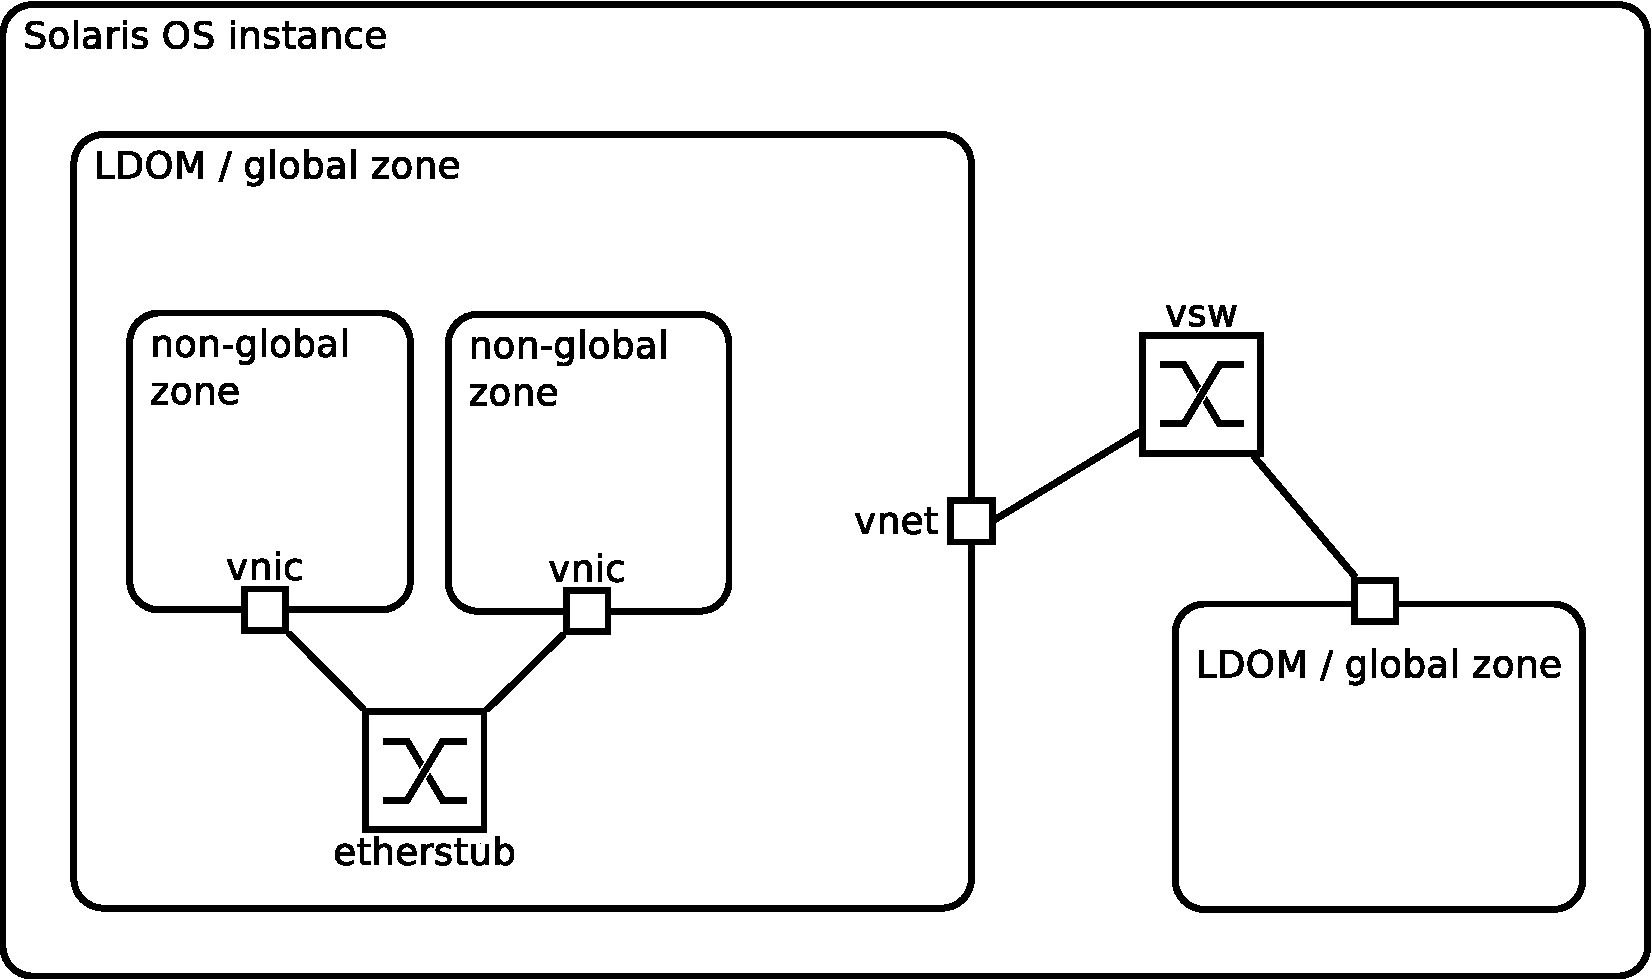
\includegraphics[width=.7\textwidth]{img/solaris/full-featured.pdf}
        \end{center}

        \caption{The variety of resources that can be virtualized with Solaris OS}
      \end{figure}

      As it can be seen, the Solaris operating system is accompanied by vast variety of virtualization-supporting
      subsystems. This multiplicity and flexibility makes it a promising platform for service provisioning and building
      even more abstract architectures on top of it. The following sections describe selected aspects of the system in
      more detail.


    \section{OS-level virtualization with Solaris Containers}
    \label{sec:sol:containers}

      % TODO citation for WPARs

      The concept of lightweight (OS-level) virtualization is supported by most modern operating systems. The solutions
      are either integrated into the system's kernel and accessible as soon as it is installed (Solaris Containers, AIX
      Workload partitions, BSD jails \cite{kamp}) or are provided by third-party manufacturers as kernel patches and
      utility software (OpenVZ and LXC for Linux OS). Because of awareness of other system components and integration 
      with them, it can be expected that Zones have more potential than other virtualization methods.


      \subsection{General information}
      \label{sub:}

        Zones technology was introduced as of Solaris OS 10. It provides a way of partitioning system resources and
        allows for isolated and secure application execution environment \cite{sag}. Solaris Zones, together with
        resource management functionality, constitute the Solaris Container environment.

        There are two types of zones: global and non-global. Global zone is the default one and is used to execute
        applications as well as to administer the system. Non-global zones can be created from within the global zone
        only. A single operating system instance with one global zone can host as many as 8192 non-global zones
        \cite{sag}.

        Zones can be assigned system resources such as CPU capacity, the amount of random-access memory or even maximum
        number of lightweight processes that can be running simultaneously. Also, network isolation is supported at two
        levels: basic, at the IP layer, and network isolation and advanced virtualization with fine grained quality of
        service control using the Crossbow technology.

        Each zone can run a different set of applications, with optional translation of system calls (Branded Zones
        Technology) thus emulating different operating environments \cite{sag}. The user is able to create a branded
        zone with translation of Linux system calls and run Linux-specific applications without code recompilation.

        \begin{figure}[H]
          \begin{center}
            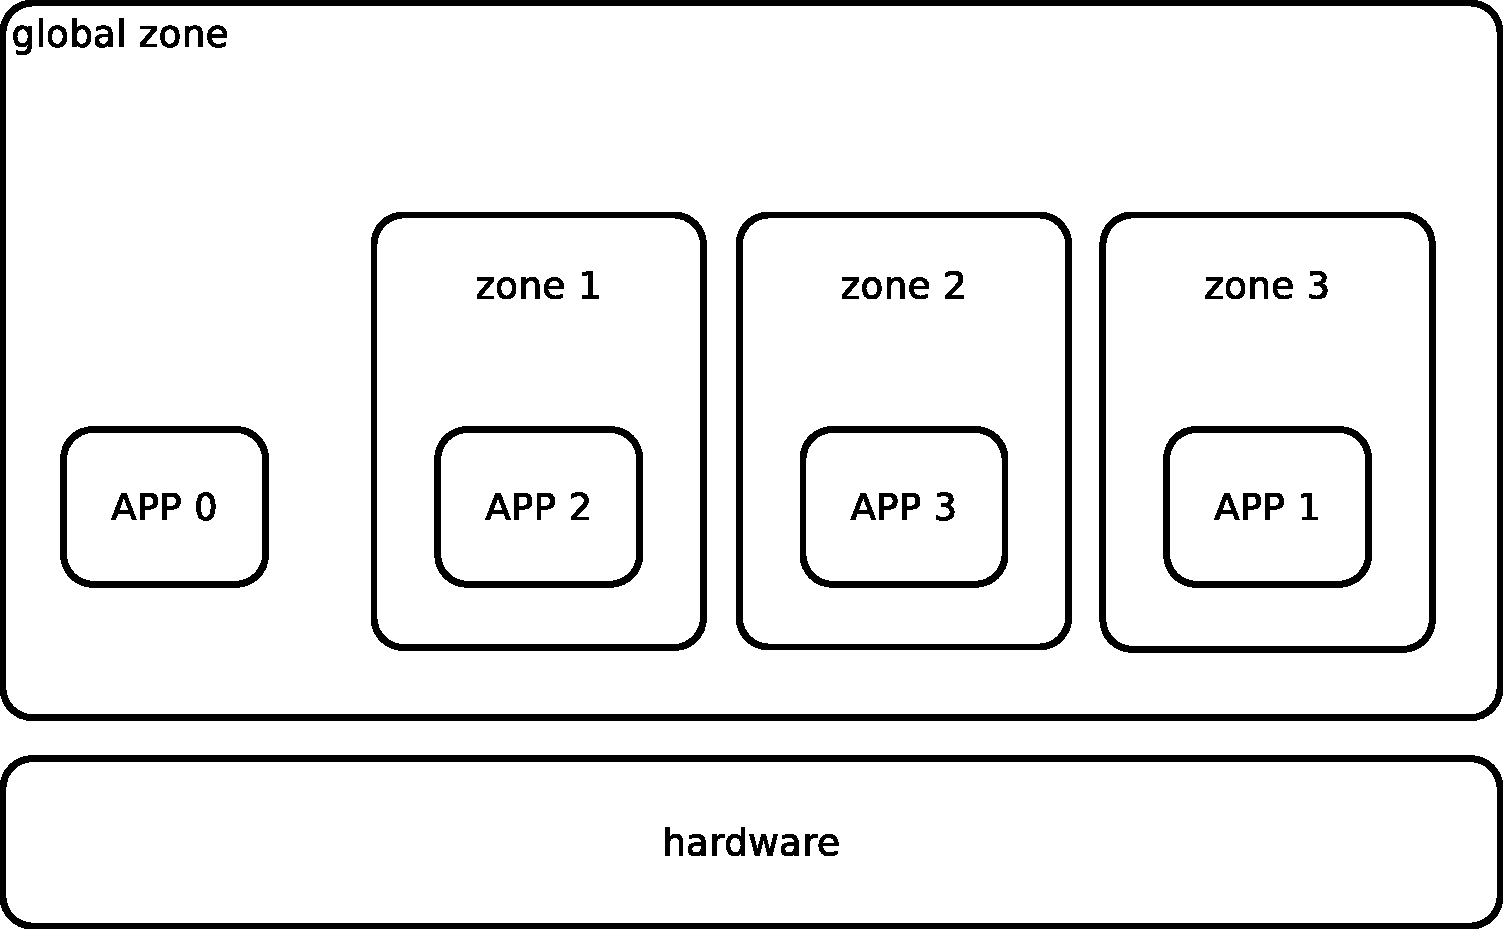
\includegraphics[width=0.7\textwidth]{img/solaris/zones-high-level.pdf}
          \end{center}

          \caption{Solaris Zones high-level view}
        \end{figure}


      \subsection{Zone lifecycle}
      \label{sub:}

        A model was created to describe the states in which each zone must exist and its possible transitions. A non-global zone can be
        in one of six states: \textit{configured}, \textit{incomplete}, \textit{installed}, \textit{ready},
        \textit{running}, \textit{shutting down or down} \cite{sag}. Figure \ref{fig:sol:lifecycle} depicts the model.

        \begin{figure}[H]
          \begin{center}
            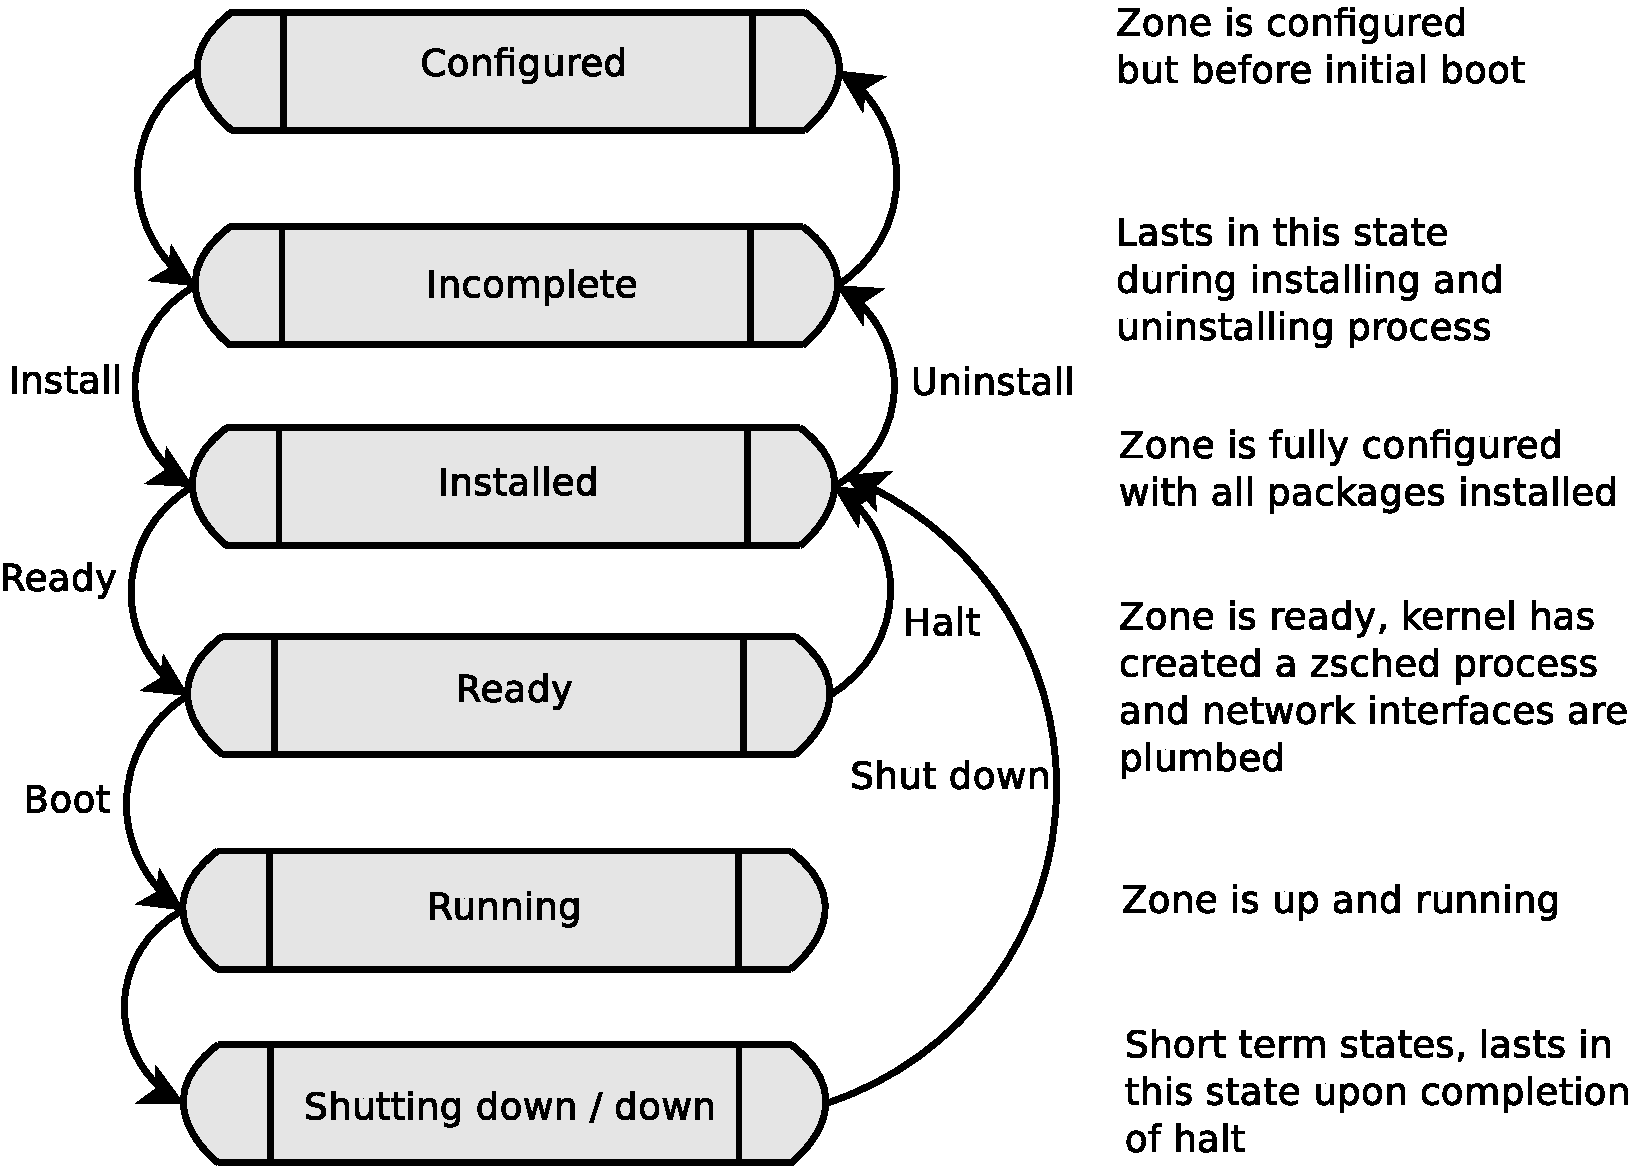
\includegraphics[width=0.7\textwidth]{img/solaris/zone_states.pdf}
          \end{center}

          \caption{Zone states and possible transitions}
          \label{fig:sol:lifecycle}
        \end{figure}


      \subsection{Isolation of processes}
      \label{sub:}

        The Containers environment offers a high level of application security and isolation. This is accomplished by
        imposing software bounds on the resource usage and introduction of additional abstraction layer over hardware.

        Every process and its children are bound to concrete zone and the assignment cannot be changed. Moreover, it is
        impossible for processes in distinct zones to monitor each other operation. They are not visible to each other
        and no interprocess communication can take place, except for network-based one, if enabled by the administrator.

        Because of the isolation, an application failure possibly affects only the processes in the containing zone.
        Assuming no interaction between processes in separate zones, the rest of the system remains intact and can
        operate normally.
        
        % TODO easier recovery, independent container management
      

      \subsection{Advantages of Containers technology when compared to non-virtualized environments}
      \label{sub:}

        The architecture of Solaris Containers makes it a competitive solution as far as systems administration and
        operation efficiency is concerned. The technology, imposing negligible overhead \cite{price}, allows to perform
        tasks that would be impossible or very hard to accomplish if traditional setup is used. Examples of such tasks
        include dynamic resource assignment, instantaneous cloning and migration of systems between physical nodes.

        The technology allows for running a number of isolated instances of operating system sharing CPU time,
        physical network bandwidth, filesystem contents and binary code. Sharing of these resources can greatly improve
        overall system efficiency and reduce the amount of occupied memory. The speed of network communication between
        different zones can also be improved thanks to ,,short-circuited'' traffic (ie. omitting the layers below IP in
        the OSI/ISO stack). The instances are able to execute applications with minimum overhead introduced mainly due
        to accessing commands and libraries through the lofs (loopback filesystem) \cite{price,fsag}.

        When using file system that supports snapshots (as, for example, ZFS), zones can be
        serialized (a snapshot of the file system can be taken) and sent over the network connection or other means of
        data transfer to another machine. There, the zone can be restored and operate as a part of the host system.

        Another important aspect of building the infrastructure with containers is resource control. The Solaris system
        makes it possible to define resource controls (rctls) at various levels, also on per-zone basis. CPU shares,
        maximum number of lightweight processes and maximum swap size are examples of resource control properties that
        can be set for a zone. This can be further extended by providing fine-grained properties at project, task and
        process levels \cite{sag}. The resource control process is dynamic - assignments can be changed as the system
        is running, without interrupting the container's normal operation. This can be of extreme importance as far
        as high-availability systems are considered.

        Containers facilitate service consolidation - all components of a system can be executed in a single machine
        with network-based communication handled entirely by the host operating system, thus eliminating the need for
        additional networking hardware and its management. The consolidated infrastructure becomes more flexible as the
        majority of administration tasks can be performed by issuing a series of terminal commands. All these factors
        make total cost of ownership lower \cite{price}.

        \begin{figure}[H]
          \begin{center}
            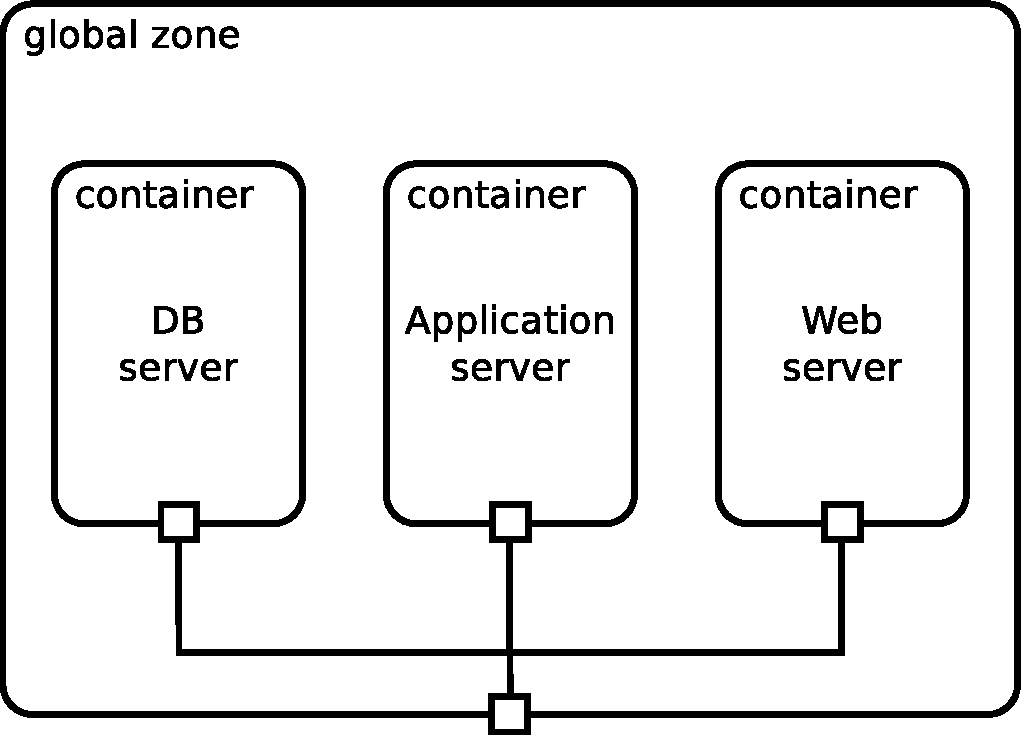
\includegraphics[width=.6\textwidth]{img/solaris/consolidation.pdf}
          \end{center}

          \caption{Service consolidation within a Solaris OS instance with internal network connectivity}
        \end{figure}


      \subsection{Virtual appliances}
      \label{sub:}

        Virtual appliance is a \textit{pre-built, pre-configured, ready-to-run (enterprise) application packaged along
        with an optimized operating system inside a virtual machine} \cite{changhua}. Solaris Zones, together with other
        components of the Solaris OS, constitute a complete framework that implements virtual appliance approach to
        systems management.

        The main problem virtual appliances can solve is the complexity and duration of application deployment process.
        In general, a service deployment can be described as comprising the following stages: preparation (learning the
        dependencies), pre-installation, installation and post-installation. With traditional (non-virtualized)
        approach, these stages have to be repeated every time a service is deployed on different machines.

        \begin{figure}[H]
          \begin{center}
            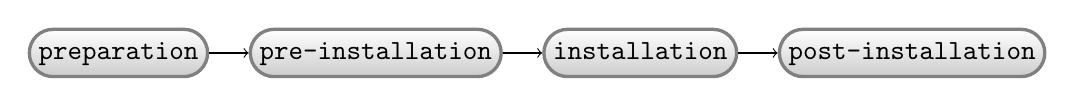
\begin{tikzpicture}[start chain,
                                node distance=5mm,
                                every node/.style={on chain, join, terminal},
                                every join/.style={->},
                                text depth=.25ex]

              \node {preparation};
              \node {pre-installation};
              \node {installation};
              \node {post-installation};
            \end{tikzpicture}
          \end{center}

          \caption{Traditional application deployment stages.}
        \end{figure}

        % TODO verify the stages

        Virtual appliance approach makes it possible to reduce deployment time significantly \cite{changhua}. This is
        achieved by performing most of the deployment stages once and storing the configured environment in a virtual
        appliance. The appliance can then be moved to publicly-available repository for actual deployment on host
        systems.

        \begin{figure}[H]
          \begin{center}
            \begin{tikzpicture}[node distance=5mm]

              { [start chain, every node/.style={terminal, on chain, join, text width=3cm}, every join/.style={->},
              align=center]

                { [every on chain/.style={text width=3.5cm}, text depth=.25ex, align=center]

                  \node (prep)                 {preparation};
                  \node (pre)  [below=of prep] {pre-installation};
                  \node (ins)  [below=of pre]  {installation};
                  \node (post) [below=of ins]  {post-installation};
                }

                \node (pub)  [right=of post] {appliance publication};
                \node (act)  [right=of pub]  {appliance retrieval and activation};
                \node (adj)  [right=of act]  {configuration adjustment};
              }

              \begin{pgfonlayer}{background}
                \node [terminal] (background) [fit=(prep) (post), style=terminal] {};
              \end{pgfonlayer}

            \end{tikzpicture}
          \end{center}

          \caption{Deployment process with virtual appliances. Stage 1 is executed once.}
        \end{figure}

        It is possible to prepare sets of virtual appliances containing traditional services (such as application
        servers, database servers or media servers) as well as highly specialized networking-focused appliances that can
        act as routers, firewalls or load balancers. These Virtual (Network) Appliances, together with other components
        provided by Solaris OS,  can be leveraged to build fully virtual network topologies.

        \begin{figure}[H]
          \begin{center}
            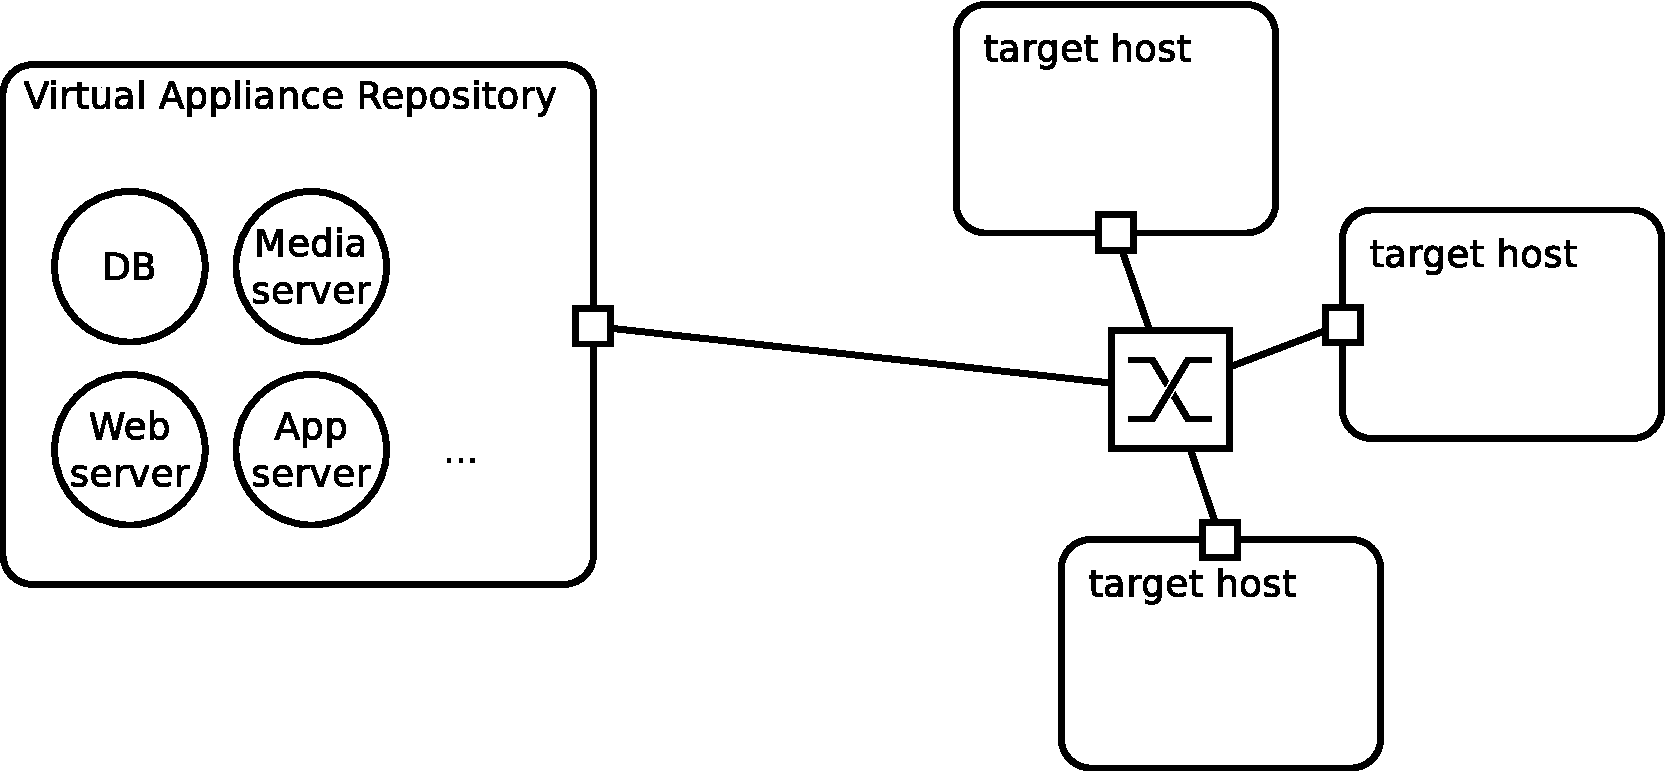
\includegraphics[width=.7\textwidth]{img/solaris/virtual-appliance-infra.pdf}
          \end{center}

          \caption{An example of infrastructure utilizing virtual appliances with appliance repository.}
        \end{figure}


    \section{Crossbow - network virtualization technology}
    \label{sec:sol:xbow}

      % TODO when introduced? +citation

      It is generally acknowledged that Crossbow was invented in China in 341 B.C but it was in middle ages when 
      it earned its recognition. Very easy in use and simultaneously very effective. The Solaris Crossbow mechanism 
      for QoS are just like real crossbows, very efficient in comparison to other existing QoS mechanisms and this
      similarity indicates the project name origin.


      \subsection{Crossbow architecture}

        One of the most important conditions in terms of network virtualization is that network traffic should be
        insulated between virtual machines. This kind of isolation can be achieved by having a dedicated physical NIC,
        network cable and port from the switch to the virtual machine itself. Moreover, switch must also ensure
        sustainability on every port. Otherwise, virtual machines will definitely interfere with each other \cite{crossbow}.
        
        In a particular case when a physical NIC has to be shared between virtual machines the most promising solution is
        to virtualize NIC hardware and the second layer of the OSI/ISO stack where sharing is fair and interference
        will be avoided. These approach was adapted in the Crossbow architecture in the Solaris OS \cite{crossbow}.
        
        Traffic separation is achieved with fundamental blocks of new architecture which are Virtual NICs (VNICs)
        created by partitioning physical NIC. A VNIC can be created over NIC or Etherstub and
        be dynamically controlled by the bandwidth and CPU resources assigned to it
        \cite{crossbow,network_virtualization}. New architecture after introducing new networking features combined with
        existing features like Solaris Containers, resource control can be presented as following:

        \begin{figure}[H]
          \begin{center}
            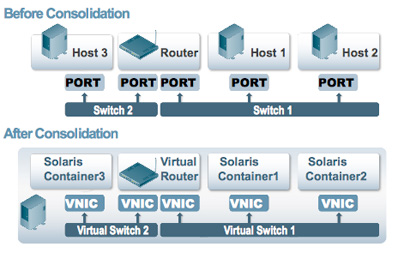
\includegraphics[width=.7\textwidth]{img/crossbow.jpg}
          \end{center}

          \caption{The Solaris Crossbow network virtualization enhancement, source: http://www.net-security.org/images/articles/crossbow.jpg}
        \end{figure}

        The crossbow architecture has introduced fully parallel network stack structure. Each stack could be seen as
        an independent lane (without any shared locks, queues, and CPUs) therefore network isolation is guaranteed.
        Key concept is hardware classification performed by the NIC over which VNIC was created.  Each lane has a
        dedicated buffer for Transmit (Tx) and Receive (Rx) ring. In case when load exceeds assigned limit packets must
        be dropped as it is wiser to drop them than to expend OS CPU resources \cite{crossbow}.

        \begin{figure}[H]
          \begin{center}
            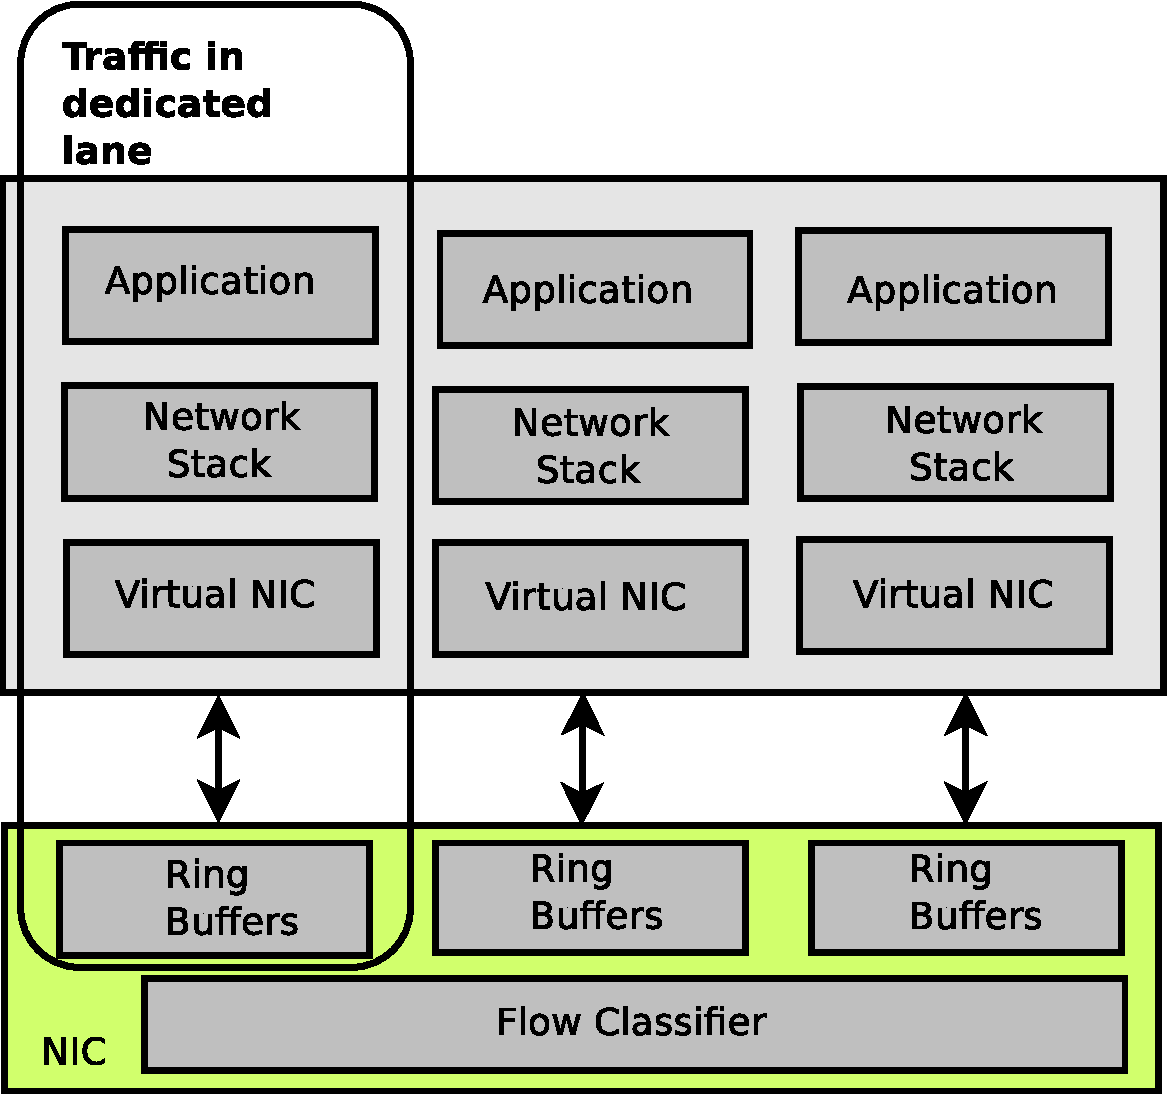
\includegraphics[width=0.5\textwidth]{img/crossbow-traffic-dedicated-line.pdf}
          \end{center}

          \caption{Dedicated lanes in the Crossbow architecture}
        \end{figure}

		
      \subsection{Virtualization lanes}

        Virtualization lane is the most key component in the Crossbow architecture. Each lane consists of some dedicated
        hardware and software that might be used to handle specific type of traffic. It usually would be composed of: 

        \begin{enumerate}
          \item NIC resources (receive and transmit rings, interrupts, MAC address slots),
          \item Driver resources (DMA bindings),
          \item MAC layer resources (data structures, execution threads, locks).
        \end{enumerate}
        
        A virtualization lane can be one of two types, hardware-based or software-based.

        
        \subsubsection{Hardware-based virtualization lanes}
        
          This type requires ability to partitioning resources from NIC. The minimum requirement is that a
          hardware-based lane should must have a dedicated receive ring.  Other resources such as transmit lane can be
          exclusive or shared between lanes. Each virtual machine could have one or more lanes assigned and the incoming
          packets would be distributed among them based on even scheduling unless some administrative polices where
          created, such as priority or bandwidth limit \cite{crossbow}.		

        
        \subsubsection{Software-based virtualization lanes}
        
          In case when NIC runs out of hardware-based virtualization lane, receive and transmit rings may be shared by
          multiple VNICs. The number of software-based virtualization lanes also often called softrings is unlimited.
          The main disadvantage of software-based lanes is the lack of fairness and isolation which in fact is provided
          in hardware-based lanes. The received and sent rings may work also in mix mode, whereas some of the rings may
          be assigned to software and some may be assigned to hardware based lanes \cite{crossbow}.	
			
      \subsection{Dynamic polling}	
        
        The Crossbow architecture proposed two types of working modes. Currently used mode is determined by traffic and
        load. Under low load, where the rate of arriving packets is lower than time of packet processing, a lane works in
        the interrupt mode which means that receive ring generates an interrupt when new packet arrives. However, when
        the backlog grows, the line switches to dynamic polling mode in which a kernel thread goes down to the receive
        ring in the NIC hardware to extract all outstanding packets in a single chain. Key aspect is that every
        virtualization lane works independently and transparently from each other. Usually only three threads are used
        per lane \cite{crossbow}:
        
        \begin{enumerate}
          \item Poll thread which goes to the NIC hardware to get all packet chain,
          \item Worker thread which is responsible for protocol processing (IP and above) or delivers packets to virtual
                machine. Thread performs also any additional transmit work which is a natural 
                requirement some concrete protocol, such as processing TCP packets that require sending ACK packets,
          \item Transmit thread that is activated when if packets are being sent after transmit side flow control relief
                discharge, or after retrieving transmit descriptor. Application or virtual 
                machine can transmit any packets without performing queuing because of flow control or context switching.
        \end{enumerate}


      \subsection{Virtual switching}
        
        Virtual switches are always created implicitly when the first VNIC is defined under existing NIC and could never
        be accessed directly nor be visible by any user (even administrator) \cite{crossbow2}. 
        
        \begin{figure}[H]
          \begin{center}
            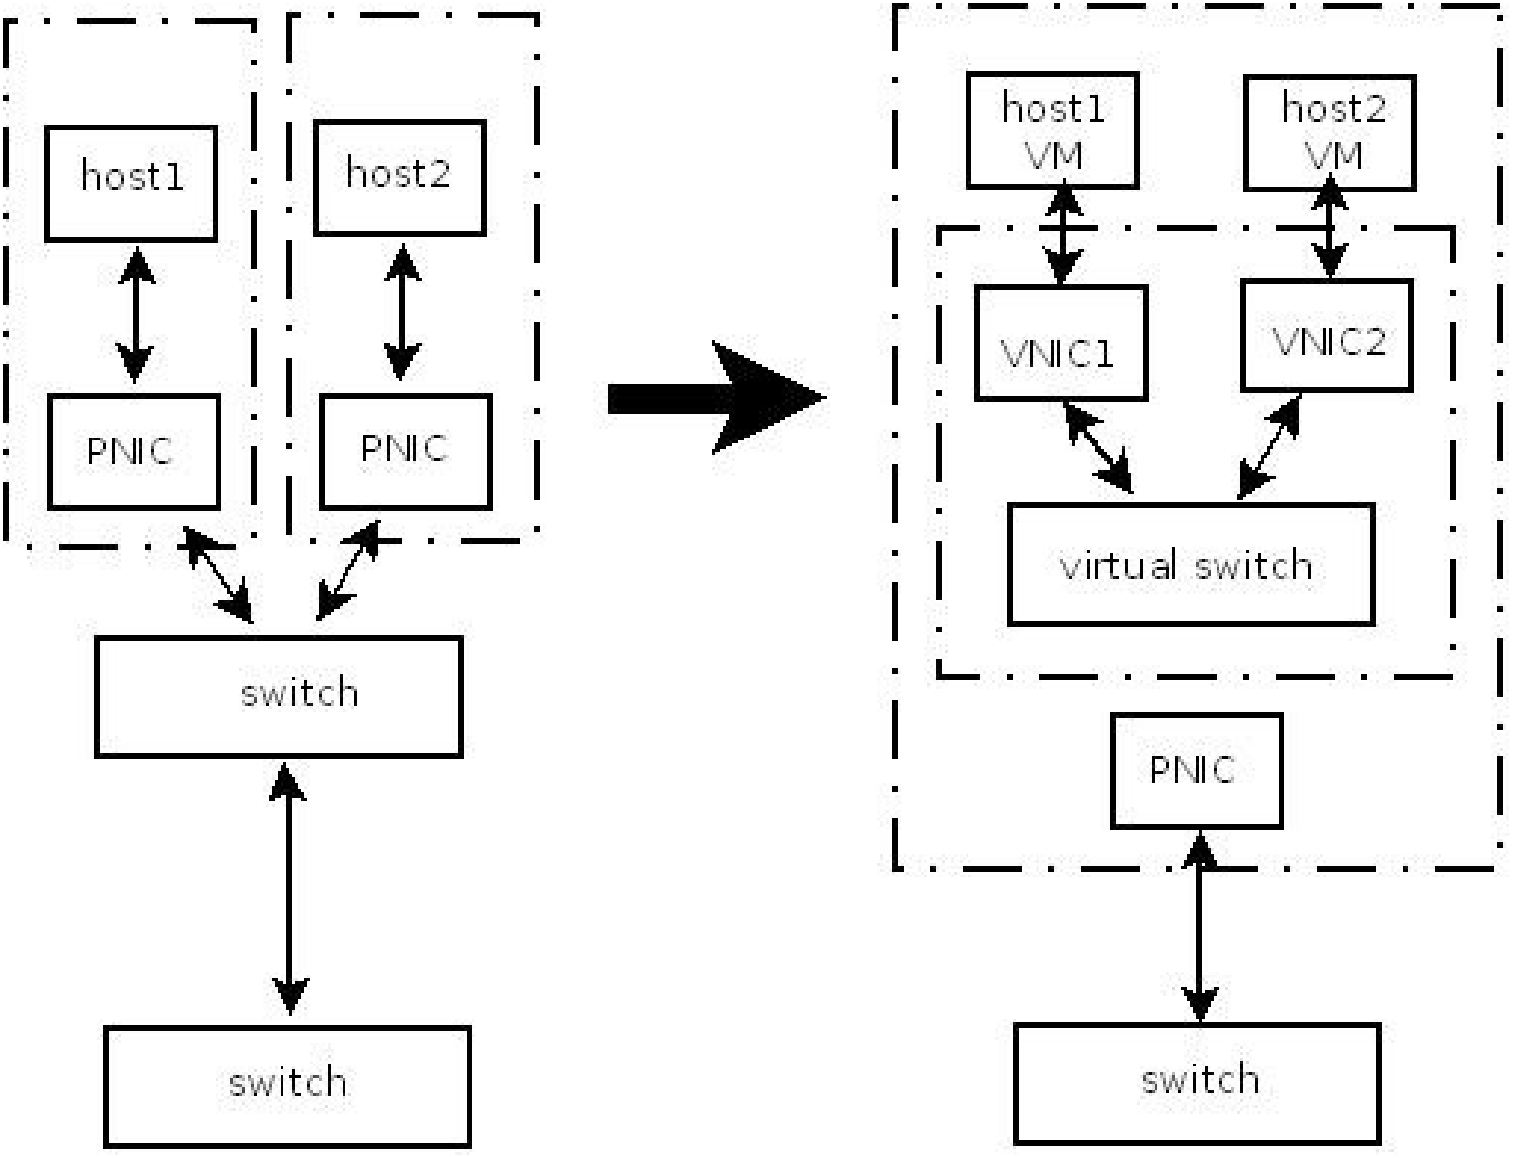
\includegraphics[width=.7\textwidth]{img/physical_and_virtual_switches_mapping.pdf}
          \end{center}

          \caption{Mapping between physical and virtual network building elements}
        \end{figure}
        
        Semantics assured by virtual switches is the same as provided by physical switches: 

        \begin{enumerate}
          \item VNICs created on top of the same NIC can send packets to each other,
          \item Broadcast packets received by the underlying NIC are distributed to every single VNIC that was defined
                on the top of this NIC,
          \item Broadcast packets sent by one of the VNICs is distributed to all VNICs defined on the top of the same
                NIC and to the NIC for further transmission as well,
          \item In terms of multicast network traffic multicast group membership is monitored and used for distributing
                packets to appropriate VNIC.
        \end{enumerate}

        Data Link Layer connectivity between VNICs is available only when they were defined on top of the same NIC. 

	
      \subsection{Crossbow components}

        The Crossbow specification describes three major components: VNICs, Etherstubs and Flows. This section gives an
        insight into their application and usage.

                
        \subsubsection{VNICs}
        
          Virtual NICs (VNICs) each containing their own lane are the key element in crossbow architecture. There is no
          difference between NIC and VNIC in administration, as they are all treated as data links. Every VNIC has an
          assigned lane and flow classifier which classifies received packets by VNIC's MAC address and sometimes by the
          VLAN tag.  If created with a VLAN tag, protocols like GVRP or MVRP may be used to register the VLAN tag with
          the physical switches too \cite{crossbow}.	

          In terms of sharing bandwidth, Crossbow enables administrative control of bandwidth for every single VNIC. The
          bandwidth of the link is implemented by regulating the periodic intake of incoming packets per dedicated lane.
          The network stack allows only as many packets as it was assigned to specific VNIC. The lane picks more packets
          when the next period begins. In case of regulating the speed of transmited bandwidth it is much easier as the
          network stack can either control the application that is generating the stream of packets or just drop the
          excessive amount of packets.  These mechanisms are also used in flows QoS described and discussed later in
          this paper \cite{crossbow}.


        \subsubsection{Etherstubs}

          As it was mentioned before, the MAC layer provides the virtual switching capabilities which allow VNICs to be
          created over existing physical NICs.  In some cases, creating virtual networks without the use of a physical
          NIC is more welcomed than creating over physical NICs. In that case VNICs would be defined on the top of
          pseudo NICs.  The Crossbow provides these kind of elements which are called Etherstubs. These components could
          be used instead of NICs during creation of VNICs \cite{crossbow}.


        \subsubsection{Flows}

          Flows are additional instruments created to allow easier network traffic administration. They might be used in
          order to provide bandwidth resource control and priority for protocols, services, containers. Virtual
          networks can be described to maintain isolation and different network properties, and define flows to manage quality
          of service \cite{network_virtualization}.

          Defined flow is a set of attributes based on Layer 3 and Layer 4 headers of the OSI/ISO model which are then
          used to identify protocol, service or virtual machine.  Flows assigned to a link must be independent therefore
          before adding new one its correctness is checked. Input and output packets are matched to flows in very
          efficient manner with minimal performance impact.

          \medskip

          Crossbow flows can be created with one of the following sets of attributes:

          \begin{itemize}
            \item Services (protocol + remote/local ports),
            \item Transport (TCP, UDP, SCTP, iSCSI, etc),
            \item IP addresses and IP subnets,
            \item DSCP field.
          \end{itemize}

          For each flow the following properties can be set \cite{flows2}: 

          \begin{itemize}
            \item bandwidth,
            \item priority.
          \end{itemize}

          \medskip

          

          \textbf{flowadm} is the console command used to create, modify, remove or to display network bandwidth and
          priority limits assigned to a particular link. 


      \subsection{Running examples of flowadm and dladm command}

        \textbf{dladm} and \textbf{flowadm} are two basic administrative commands for dealing with the Crossbow's
        components. Below a few general examples of their usage are presented.
  
        \textbf{dladm} is the admin command for crossbow datalinks elements management. Below a few examples of VNICs,
        Etherstubs management commands are presented and how bandwidth and priority values might be assigned to these
        elements.
  
        \begin{itemize}
          \item \# dladm create-vnic vnic1 -l e1000g0 - creates new VNIC \textbf{vnic1} over existing NIC \textbf{e1000g0},
          \item \# dladm create-etherstub ether00 - creates new Etherstub \textbf{ether00},
          \item \# dladm show-linkprop vnic11 - lists all properties assigned to \textbf{vnic11} link,
          \item \# dladm set-linkprop -pmaxbw=1000 vnic11 - assignes 1Mbps bandwith limit to \textbf{vnic11} link,
          \item \# dladm set-linkprop -ppriority=low vnic11 - assignes low priority to \textbf{vnic11} link.
        \end{itemize}
  
        More examples can be found in \textbf{man dladm}.

        \medskip

        \textbf{flowadm} is the admin command for flow management. It might be used as follows:     

        \begin{itemize}
          \item \# flowadm show-flow -l e1000g0 - displays all flows assigned to link \textbf{e1000g0},
          \item \# flowadm add-flow -l e1000g0 -a transport=udp udpflow - creates new flow assigned to link
                \textbf{e1000g0} for all udp packets.
        \end{itemize}

        More information about \textbf{flowadm} and \textbf{dladm} tools can be found in manual.


      \subsection{Crossbow and Differentiated Services - interoperability}
      \label{sub:sol:diffserv}

        The Crossbow technology is designed to work inside single operating system instance, there are no mechanisms
        meant to cope with problems that arise when dealing with installations spanning multiple physical machines
        connected with traditional (non-virtual) network. Crossbow's flows are, by design, relatively simple (when
        compared to DiffServ) but more efficient as far as receive performance is considered \cite{xbow-vertically}.
        Crossbow, unlike DiffServ, does not require special hardware, although if it is present it can boost overall
        operation performance \cite{xbow-vertically}.

        DiffServ, on the other hand, provides sophisticated QoS mechanisms that require proper hardware (DiffServ-aware
        routers) to be present for it to work. DiffServ is standardized (RFC 2475) and offers a multiplicity of
        classification, marking, policing and traffic shaping alternatives \cite{rfc2475}. Special fields (called DSCP)
        contained in IP packet's header are used to carry processing-related information with packets. The approach can
        be used with complex networks, comprising a number of routers with QoS awareness.

        These two environments complement one another rather than compete. Crossbow supports flow matching based on the
        DSCP field value. DSCP field generation is planned but not yet supported. It is possible (although, at the
        moment, only partially) to integrate these and build a comprehensive end-to-end networking solution with QoS
        support and virtualized components.

        \begin{figure}[H]
          \begin{center}
            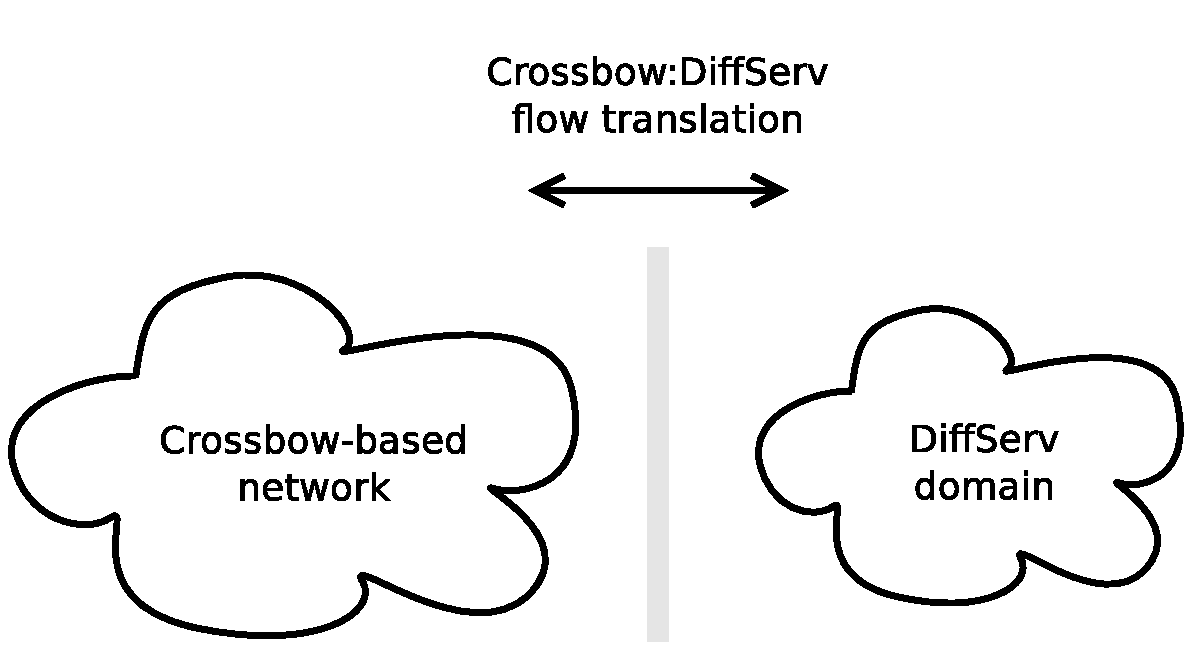
\includegraphics[width=.7\textwidth]{img/solaris/xbow-diffserv.pdf}
          \end{center}

          \caption{DiffServ integration using Crossbow-provided mechanisms}
        \end{figure}


    \section{Resource control}
    \label{sec:sol:res}

      Nowadays existing operating systems must provide mechanisms for response to the varying resource demands per
      workload which is an aggregation of processes of an application. By default resource management features are not
      used and system gives equal access to resources. When necessary, it is possible to modify this default behaviour
      with respect to different workloads. It is allowed to:

      \begin{enumerate}
        \item Restrict access to specific resource,
        \item Offer resources to workloads on a preferential basis,
        \item Isolate workloads from each another.
      \end{enumerate}
	
      Resource is any part of computing system that may be modified in order to change application behaviour. Resource
      management enables more effective resource utilization and avoid wasting available ones due to load variability.
      Reserving additional capability during off-peak periods and effective sharing resources definitely increases
      application performance.

      Most of the operating systems limited the resource control just to per-process control, whereas Oracle Solaris has
      extended this concept to the task, project and zone. Due to introducing granularity levels processes, tasks, and 
      zones are efficiently controlled from excessive resource consumption. All these enhacements are available thanks 
      to resource controls (rctls) facility \cite{oracle_admin_guide}.
      
      Solaris Operating System introduced three types of resource management control mechanisms:

      \begin{enumerate}
        \item constraints - allows defining set of bounds on used resources for a workload,
        \item partitioning - enables binding subset of system's available resources to specific workload,
        \item scheduling - involves predictable algorithm making sequence of allocation decisions at specific intervals.
      \end{enumerate}

      Hierarchical architecture allows defining set of resource control sets on each level. However, if more than one is
      assigned to a resource, the smallest container's control level is enforced \cite{oracle_admin_guide}. 

      \begin{figure}[H]
        \begin{center}
          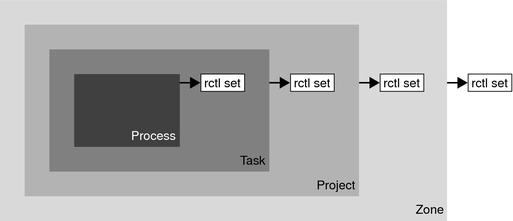
\includegraphics[width=.7\textwidth]{img/rctrl.png}
        \end{center}
        
        \caption{Solaris system multilevel architecture and its resource control sets (source: http://oracle.com)}
                          %@todo add preceise url}
		  \end{figure}


      \subsection{Accounting}
      \label{sub:sol:acct}

        Highly configurable accounting facility is provided as part of the system. Its role is to gather historical
        usage records of system and network resources. There are two levels accounting can work on in Solaris
        OS - basic and extended. Basic accounting allows for per-zone and per-project statistics gathering while
        extended accounting facility makes it possible to collect the data for tasks and processes. Statistics gathered
        by the extended accounting can be examined using C or Perl interface of the libexacct library \cite{sag}.

        The extended accounting facility can gather data for:

        \begin{itemize}
          \item system resources usage (per-task and per-process),
          \item flows defined with the IPQoS tools,
          \item links and flows created with Crossbow.
        \end{itemize}

        % TODO what data can be gathered?
                

    \section*{Summary}

      The chapter presented Solaris operating system with regard to resource virtualization. The stack of tools
      integrated into the system provides extensive support for virtualization techniques: Containers facilitate
      OS-level resource virtualization and Crossbow, shipped with Solaris 11, makes virtualization of networking
      resources possible. Resource control subsystem gives the administrator even more fine-grained control over
      resource utilization. Last, but not least, accounting functionality provides detailed view of resource usage
      history.

      The features mentioned above make realization of flexible, scalable and efficient systems possible. With these
      foundations, it is possible to build and consolidate complex network-oriented infrastructures that prove to be
      reliable, relatively easy to manage and adjust to changing requirements.

      Solaris 10 OS seems to be ideal cross-platform choice for customers dealing with management of high level
      services, complex system administration and high costs. It is the only open operating system which has proven
      results running from every critical enterprise databases to high performance Web farms that is why Solaris OS is
      becoming strategic platform for today's constantly growing demands towards operating systems
      \cite{solaris_operating_system}. 


  \chapter{The system architecture}

    The chapter discusses architectural aspects of the created system. First, the operating environment is discussed
    together with third-party components used to run the system. Then, general high-level view is described and
    layers of the system are presented. The remaining sections describe details of the layers.

    Section \ref{sec:arch:env} presents the context of the system. The distributed environment is described and
    basic requirements with regard to installed software are listed. Also, the way of extending the environment with
    specialized components is presented.

    Section \ref{sec:arch:over} introduces the design of the system. Main layers (or subsystems) are identified together
    with corresponding responsibilities. General aspects of layer interoperability are described.

    Section \ref{sec:arch:inst} provides in-depth description of resource instrumentation layer. Its internal design is
    presented and main classes of objects analyzed. Interactions between the objects are depicted and, finally, the
    listing showing all the crucial classes belonging to the layer follows.

    Section \ref{sec:arch:vi} describes the topmost layer of the whole system --- virtual infrastructure management. The
    layer functionality is presented, then data model used is introduced and discussed and main components of the layer
    are described together with their interdependencies and interactions. Extensive description of the layer's three
    main use-cases --- instantiation, discovery, monitoring --- follows.


    \section{Operating environment}
    \label{sec:arch:env}

      As depicted in figure \ref{fig:arch:deployment}, the system is designed to operate in a distributed environment
      --- the bottommost layer of the operating environment is an IP network of physical machines. Each of the machines
      is running an instance of Solaris Operating System with support for Crossbow technology. None of the nodes is
      favoured over the others. The instances of operating system have Java Virtual Machine deployed and are capable of
      running JMX Agent which is used to host components of the system.

      In addition to these basic specification, pure JMX Agents (i.e. agents without any components registered) can be
      enriched with third-party software and thus enable complete set of functionality implemented. With pure JMX Agents
      only single-node management is possible and limited to Crossbow networking resources. After integration with JIMS
      the system gains awareness of the whole distributed environment, has access to extensive mechanisms for
      controlling containers and can be used to create and manage complex virtual network topologies.
    
      \begin{figure}[H]
        \begin{center}
          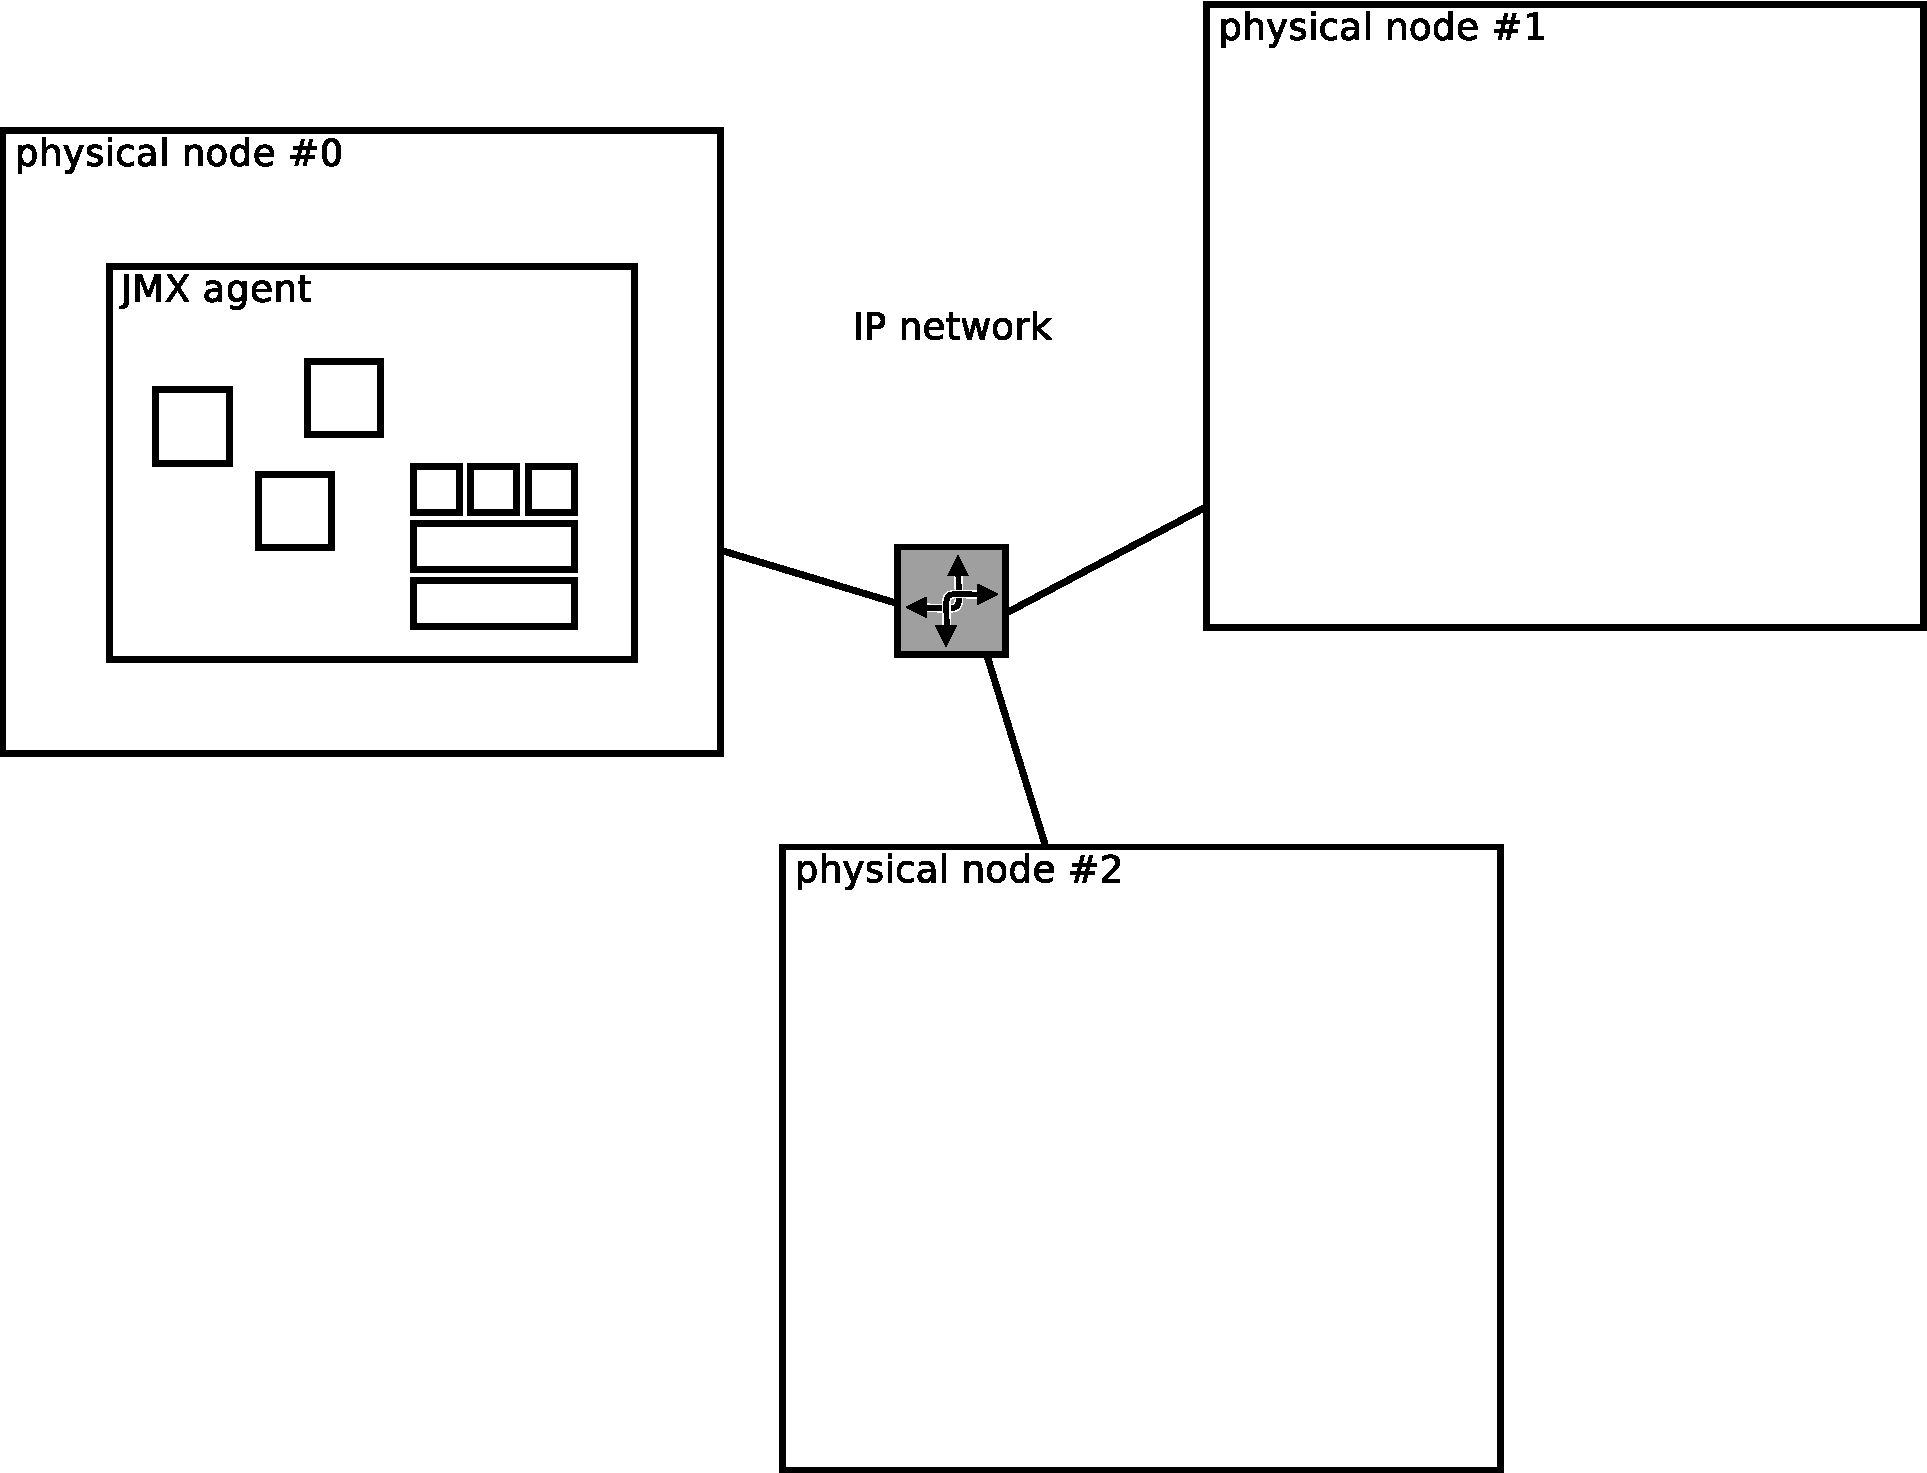
\includegraphics[width=.8\textwidth]{img/architecture/deployment.pdf}
        \end{center}

        \caption{Deployment diagram for the system}
        \label{fig:arch:deployment}
      \end{figure}


    \section{Architecture overview}
    \label{sec:arch:over}

      When considered at a very high level, the architecture of the system as a whole is layer-based. There are three
      main layers, each specifying a set of its own interfaces. The higher the layer is placed in the stack, the more
      complex interface it exposes. The three layers, as shown in figure \ref{fig:arch:layers}, are:

      \begin{itemize}

        \item Infrastructure management layer

              contains components that help design, instantiate and manage network topologies, \\
              can possibly span multiple physical machines, \\
              requires JIMS installation to operate,

        \item Resource instrumentation layer

              is an abstraction layer over resources provided by the underlying system, \\
              present on each of the physical hosts, \\
              network-based interoperability between nodes is not supported,

        \item Underlying resources layer

              represents all the resources made available by host operating system, \\
              can be managed with vendor-supplied low-level utilities and libraries.

      \end{itemize}

      All the operations (e.g. topology modification) performed by infrastructure management layer go down the stack
      and, after necessary transformations, result in persistent changes to underlying resources. Conversely, the state
      of low-level resources can be expressed in terms of the domain model used by the highest layer (discovery
      process).

      \begin{figure}[H]
        \begin{center}
          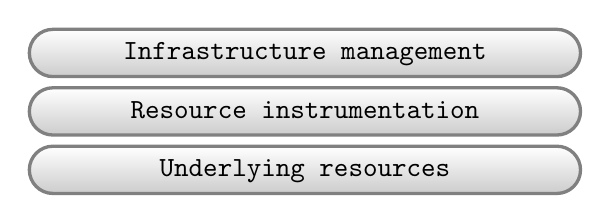
\begin{tikzpicture}[start chain,
                              node distance=1mm,
                              every node/.style={terminal, minimum width=7cm},
                              text depth=.25ex]

            \node (infr)                 {Infrastructure management};
            \node (inst) [below=of infr] {Resource instrumentation};
            \node (undr) [below=of inst] {Underlying resources};
          \end{tikzpicture}
        \end{center}

        \caption{Layered system architecture}
        \label{fig:arch:layers}
      \end{figure}


    \section{Crossbow resources instrumentation}
    \label{sec:arch:inst}

      The main responsibility of resource instrumentation subsystem is to provide a consistent way to create and manage
      resources of the underlying operating system. This general-purpose abstraction layer can easily be expanded when
      needed and further leveraged to build more sophisticated systems on top of it.


      \subsection{Separation of concerns}

        There are two classes of objects present at this level (figure \ref{fig:arch:manent}) --- Entity objects that
        are abstractions representing resources of specific type and exposing appropriate interfaces, and Manager
        objects used to perform basic coarse-grained operations (such as creation, deletion, modification) on resources
        they manage.

        \begin{figure}[H]
          \begin{center}
            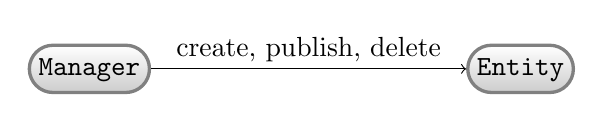
\begin{tikzpicture}[node distance=4cm, text depth=.25ex]

             \node (ent) [terminal] {Entity};
             \node (man) [terminal, left=of ent] {Manager}
               edge [->] node [auto] {create, publish, delete} (ent);

            \end{tikzpicture}
          \end{center}

          \caption{Manager and entity objects interoperability}
          \label{fig:arch:manent}
        \end{figure}


        \subsubsection{Entity objects}

          Entity objects represent instances of a resource type. Each entity object class exposes an interface to manage
          the resource it is associated with. Fine-grained management is possible with entity objects --- single
          properties can be accessed and manipulated (a subset of Flow public interface is presented in listing
          \ref{lst:arch:iface:flow}). \\

          \noindent
          \begin{minipage}{\textwidth}
            \lstinputlisting[caption={Selected methods of entity interface},label={lst:arch:iface:flow},language=Java]{lst/arch-iface-flow.java}
          \end{minipage}


        \subsubsection{Manager objects}

          Each manager subtype is associated with a single class of resources. The subtype can be thought of as a
          gateway exposing methods to manage collection of resources. The responsibilities of manager objects include
          resource discovery, creation, modification and removal. Managers maintain lists of resources present in the
          system and provide ways to access them (as entity objects). The resources can also be published in external
          repositories. \\

          \noindent
          \begin{minipage}{\textwidth}
            \lstinputlisting[caption={Selected methods of manager interface},label={lst:arch:iface:flowmanager},language=Java]{lst/arch-iface-flowmanager.java}
          \end{minipage}

          Sequence diagram in figure \ref{fig:arch:pub} shows the process of creating new entity object. After creation,
          the object is published in a repository to make it accessible for other components.

          \begin{figure}[H]

            \centering

            \begin{sequencediagram}

              \newthread{cli}{Client}
              \newinst[2]{man}{Manager}
              \newinst[1]{lib}{Native library}
              \newinst[1]{pub}{Publisher}

              \begin{call}{cli}{create(entity)}{man}{}
                \begin{call}{man}{create(entity)}{lib}{}
                \end{call}
                \begin{sdblock}{if publisher attached}{}
                  \begin{call}{man}{publish(entity)}{pub}{id}
                  \end{call}
                \end{sdblock}
              \end{call}
            
            \end{sequencediagram}

            \caption{Entity creation scheme with optional publication}
            \label{fig:arch:pub}
          
          \end{figure}


      \subsection{Layered design}

        Both the Manager and Entity objects share the same three-layer internal design as presented in figure
        \ref{fig:arch:laydes}. The objects themselves are exposed as Java Management Extensions beans. To implement the
        interface, either shell scripts or native libraries (or both) are used depending on the complexity of an
        operation. At the lower level, command line programs or native calls are executed, respectively.

        \begin{figure}[H]
          \begin{center}
            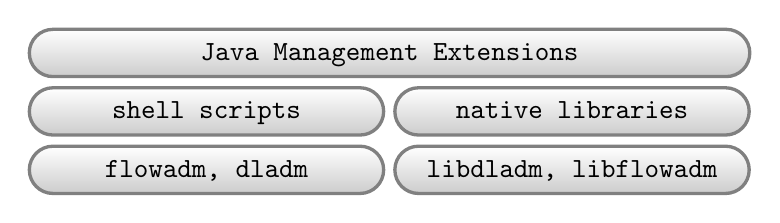
\begin{tikzpicture}[start chain,
                                node distance=1mm,
                                every node/.style={terminal, minimum width=4.5cm},
                                text height=1.5ex, text depth=.25ex]

              \node (jmx)  [minimum width=9.15cm] {Java Management Extensions};
              \node (midl) [below=of jmx.south west, anchor=north west] {shell scripts};  \node (midr) [right=of midl] {native libraries};
              \node (lowl) [below=of midl] {flowadm, dladm};                              \node (lowr) [right=of lowl] {libdladm, libflowadm};
            \end{tikzpicture}
          \end{center}

          \caption{Layered system architecture}
          \label{fig:arch:laydes}
        \end{figure}


      \subsection{Instrumented Solaris OS resources}

        All the important Crossbow resources are instrumented (Manager:Entity pairs are created). This includes NICs
        (Network Interface Cards), VNICs (Virtual Network Interface Cards), VLANs (Virtual LANs), Etherstubs and Flows.
        All the components are loosely coupled and can be used independently.

        \begin{figure}[H]
          \begin{center}
            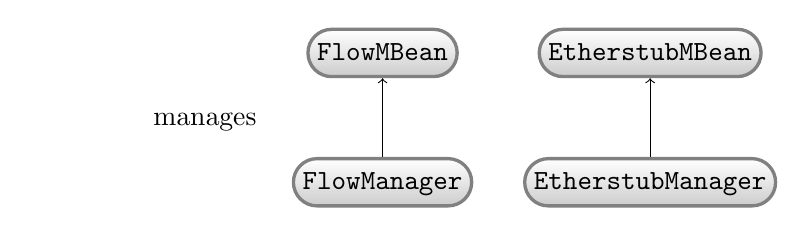
\begin{tikzpicture}[every node/.style={minimum width=4.5cm},
                                text height=1.5ex, text depth=.25ex]

              \node (eflow) [terminal] {FlowMBean};
              \node (mflow) [terminal, below=of eflow] {FlowManager}
                edge [->] node [auto] {manages} (eflow);

              \node (eether) [terminal, right=of eflow] {EtherstubMBean};
              \node (mether) [terminal, below=of eether] {EtherstubManager}
                edge [->] node [auto] {} (eether);

            \end{tikzpicture}

            \bigskip

            \begin{tikzpicture}[every node/.style={minimum width=4.5cm},
                                text height=1.5ex, text depth=.25ex]

              \node (enic) [terminal, below=of mflow] {NICMBean};
              \node (mnic) [terminal, below=of enic] {NICManager}
                edge [->] node [auto] {manages} (enic);

              \node (evnic) [terminal, right=of enic] {VNICMBean};
              \node (mvnic) [terminal, below=of evnic] {VNICManager}
                edge [->] node [auto] {} (evnic);

              \node (evlan) [terminal, right=of evnic] {VLANMBean};
              \node (mvlan) [terminal, below=of evlan] {VLANManager}
                edge [->] node [auto] {} (evlan);
              
            \end{tikzpicture}
          \end{center}

          \caption{Instrumented resources}
          \label{fig:arch:instr}
        \end{figure}
        

    \section{Virtual infrastructure management}
    \label{sec:arch:vi}

      Virtual infrastructure management subsystem is built on top of the instrumentation layer. Leveraging entity and
      manager objects and components of the JIMS project, it provides high-level mechanisms to manage and monitor
      complex network topologies and quality policies associated with them.


      \subsection{High-level functionality overview}
      \label{sub:arch:hl}

        Figure \ref{fig:arch:hl} shows main stages of the management process together with general flows of data and is
        the starting point when identifying and designing coarse-grained components. The stages presented map to
        implemented components of the system that were implemented --- User Interface to design, manipulate and monitor
        the topology, nodes responsible for discovery of available physical hosts, and mappers which translate between
        logical model and underlying resources.

        % TODO zwezic ten diagram

        \begin{figure}[H]
          \begin{center}
            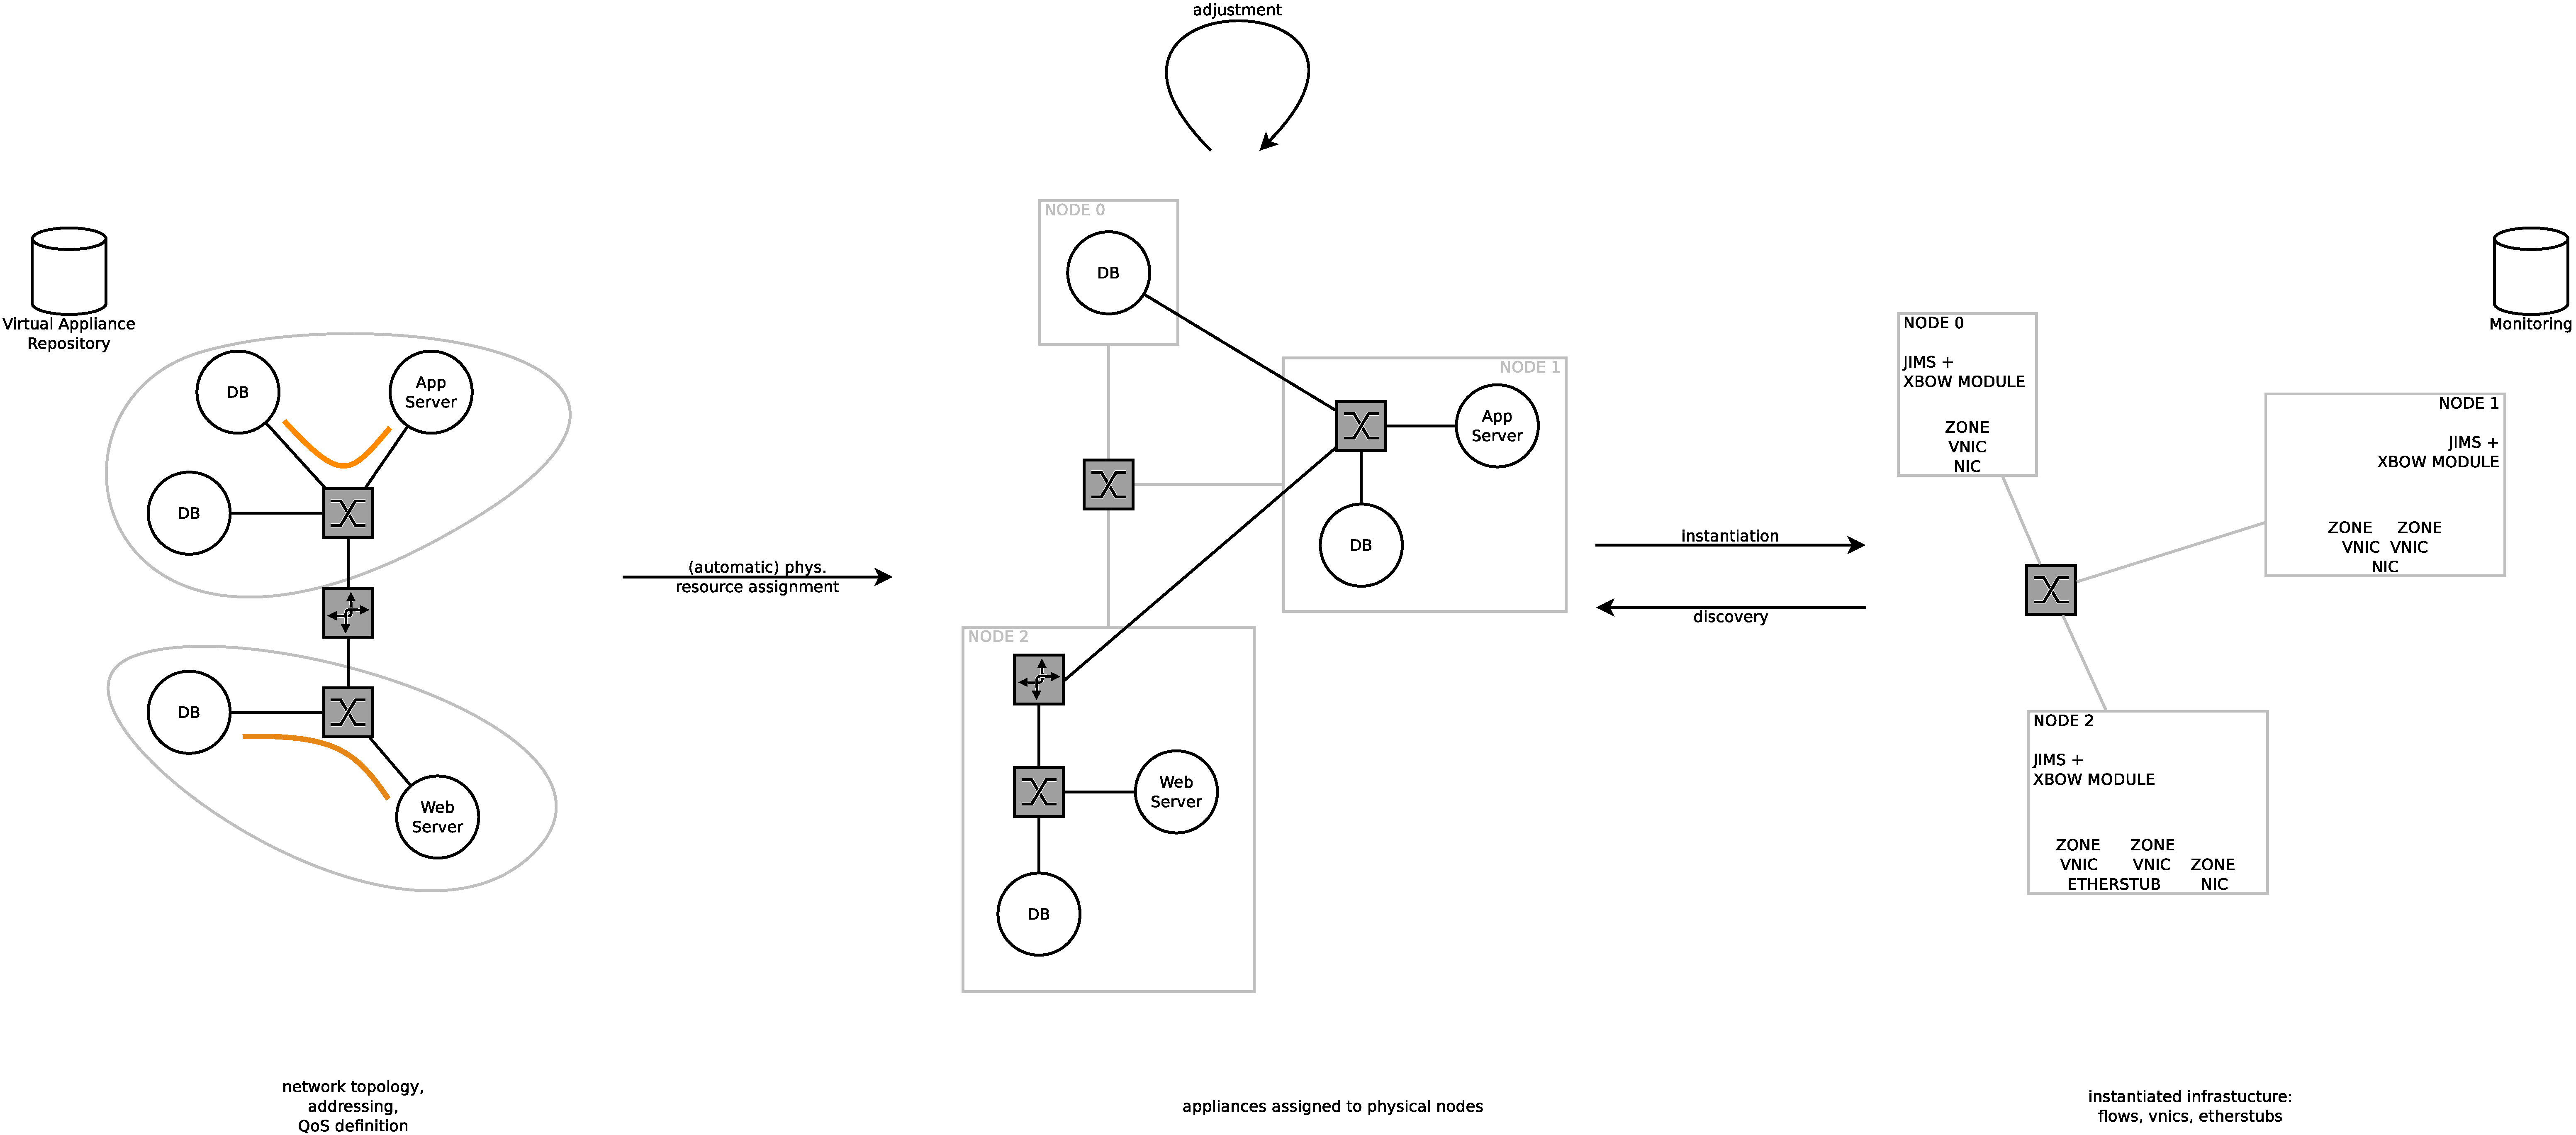
\includegraphics[width=\textwidth]{img/architecture/scope.pdf}
          \end{center}

          \caption{Main stages of operation}
          \label{fig:arch:hl}
        \end{figure}


      \subsection{Domain model and data flows}
      \label{sec:domain-model}

        Dedicated domain model was created for the virtual infrastructure management layer. It describes higher-level
        entities and operations that can be performed. The model is divided into three logical groups --- static data
        describes resources and their interdependencies, assignment model is used to denote the association between
        parts of a topology and underlying physical resources, actions model is used to express the operations that can
        be applied to elements of a topology.


        \subsubsection{Static data model}

          As far as networking domain is considered, the model covers three main aspects:

          \begin{itemize}

            \item available entities --- the set of resources that can be used to build a network topology,

                  \begin{figure}[H]
                    \begin{center}
                      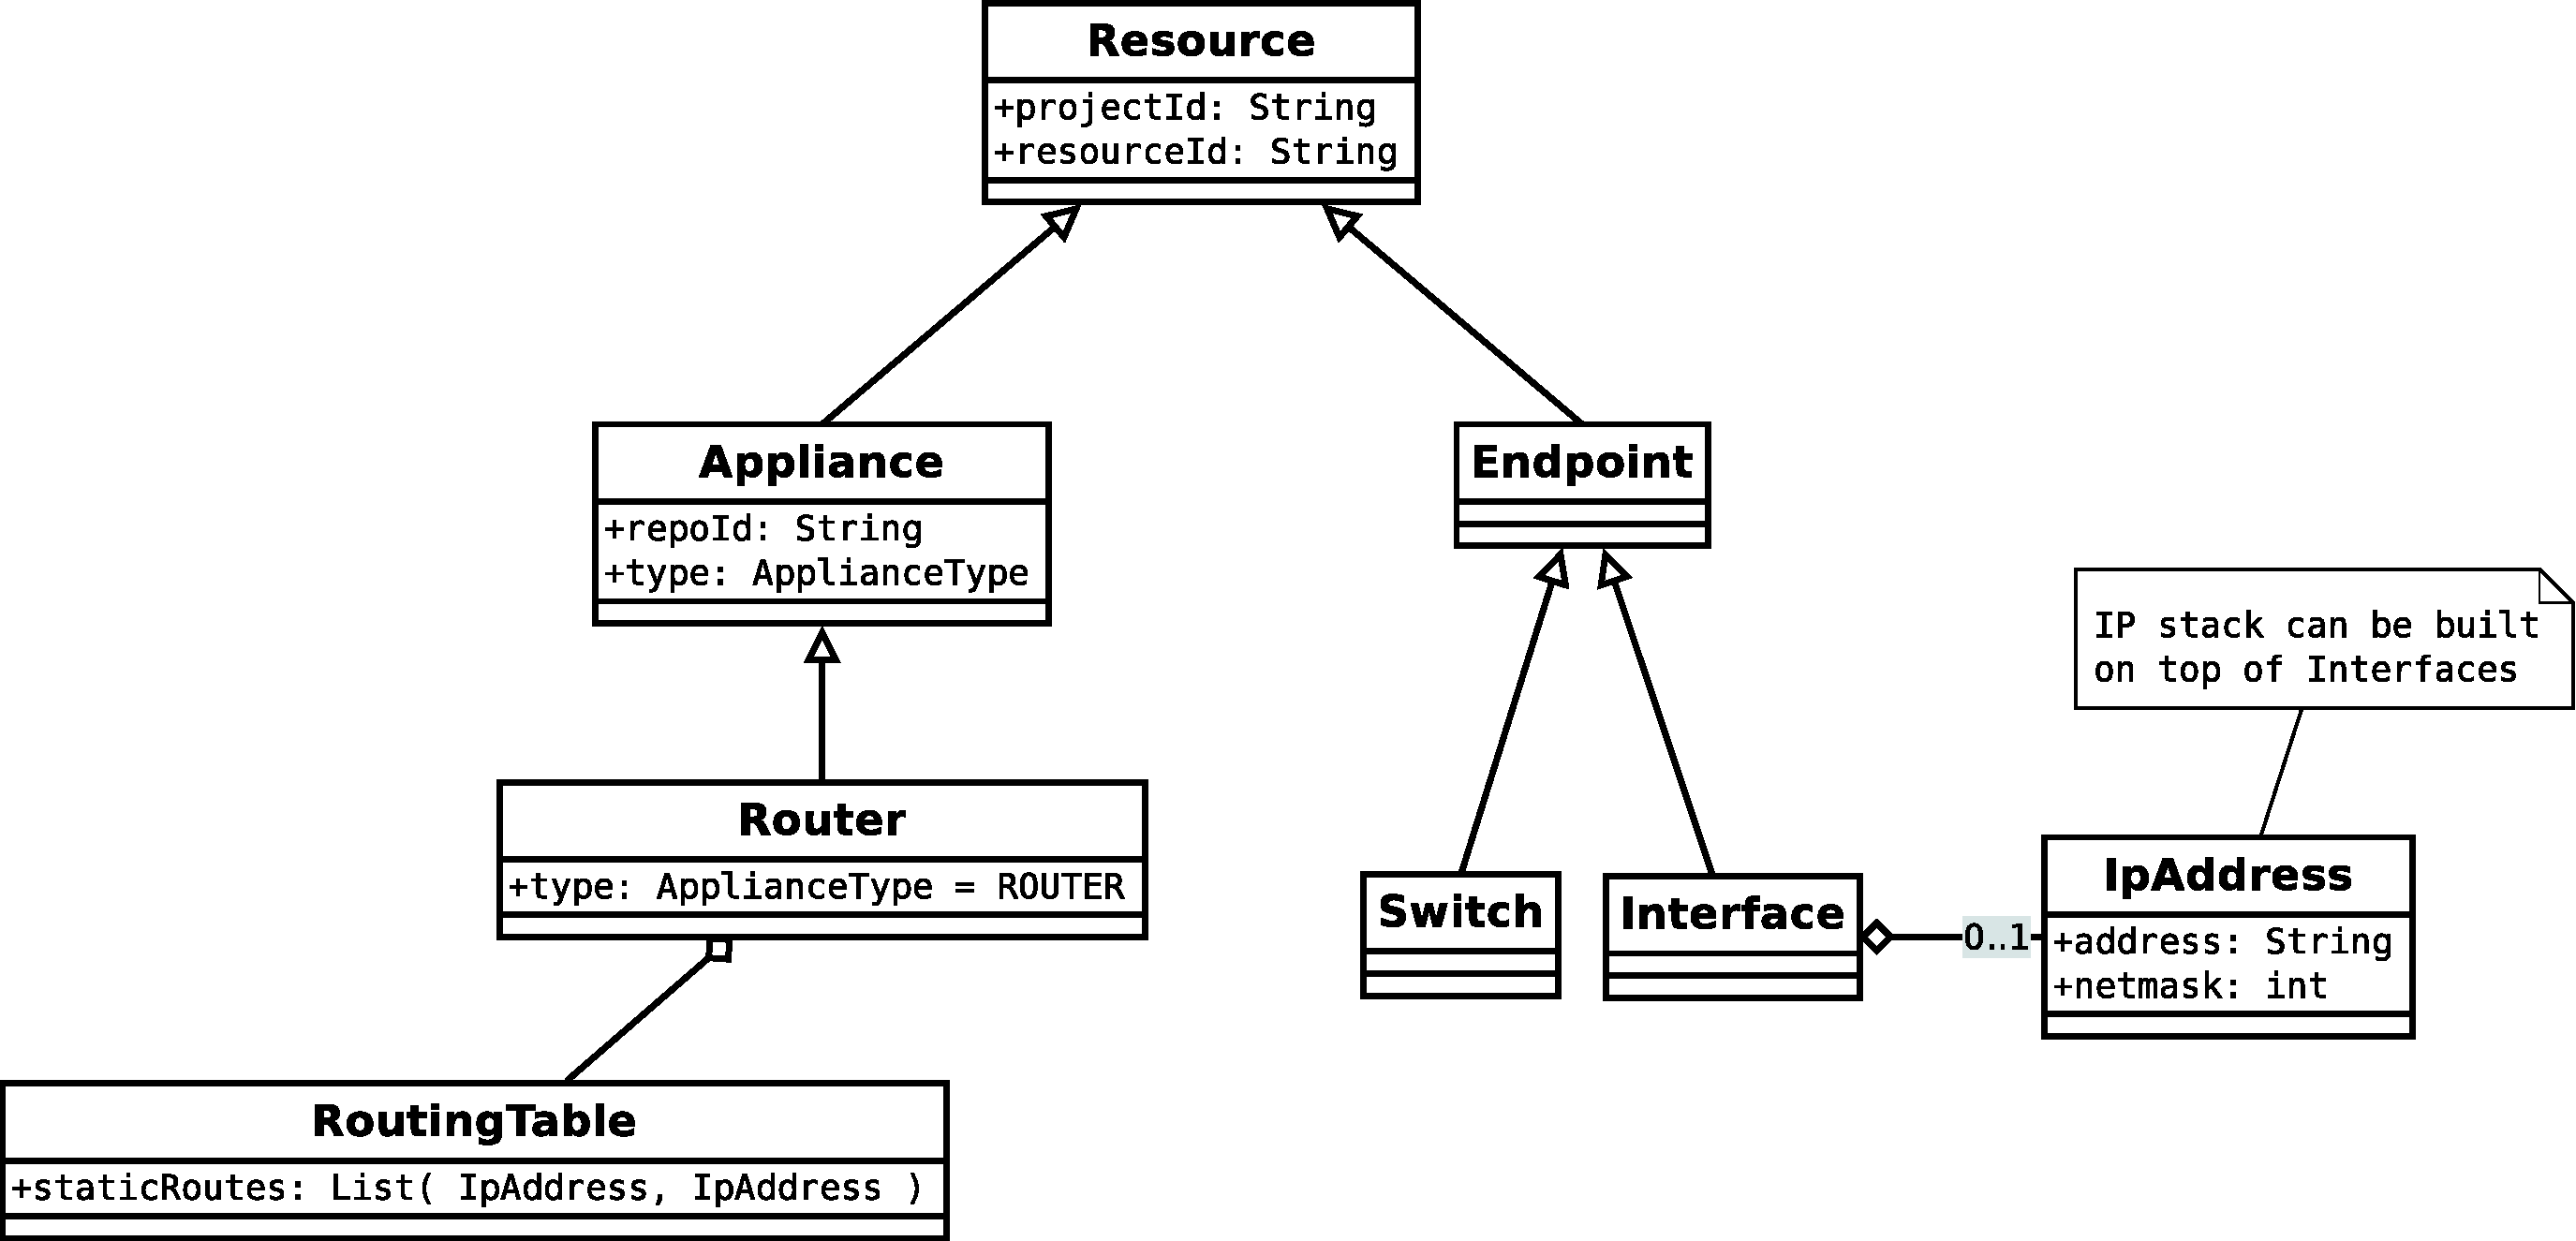
\includegraphics[width=0.7\textwidth]{img/architecture/om-entities.pdf}
                    \end{center}
                    \caption{Object model --- entities}
                  \end{figure}

            \item allowed interconnections --- reflecting a subset of real-world connections between networking
                  hardware,

                  \begin{figure}[H]
                    \begin{center}
                      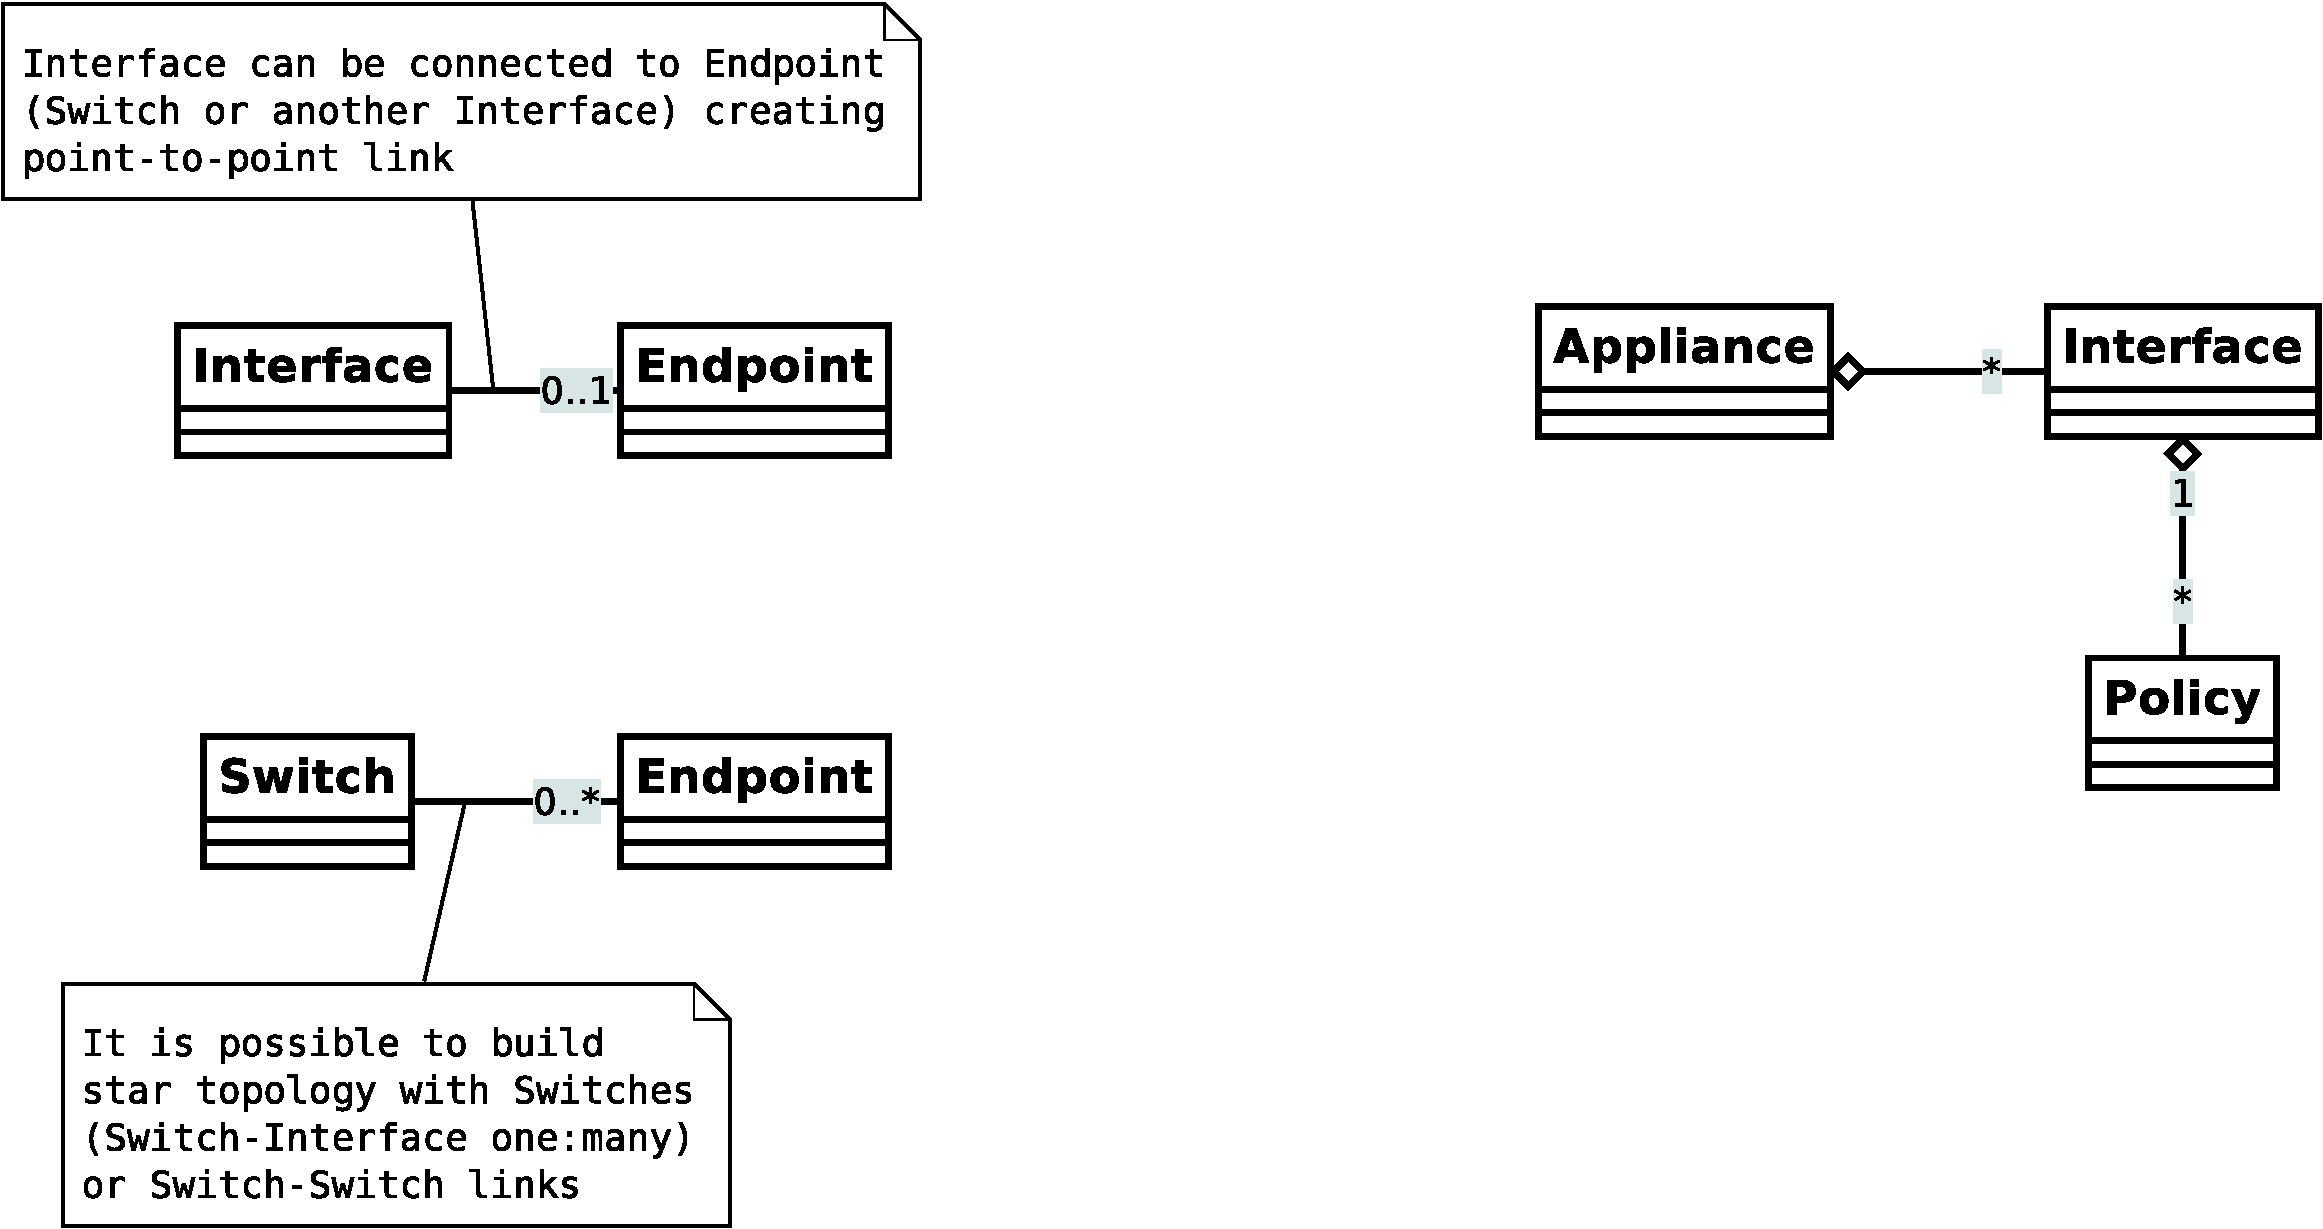
\includegraphics[width=0.7\textwidth]{img/architecture/om-ic.pdf}
                    \end{center}
                    \caption{Object model --- interconnections}
                  \end{figure}

            \item Quality of Service policies --- classify traffic and determine priorities.

                  \begin{figure}[H]
                    \begin{center}
                      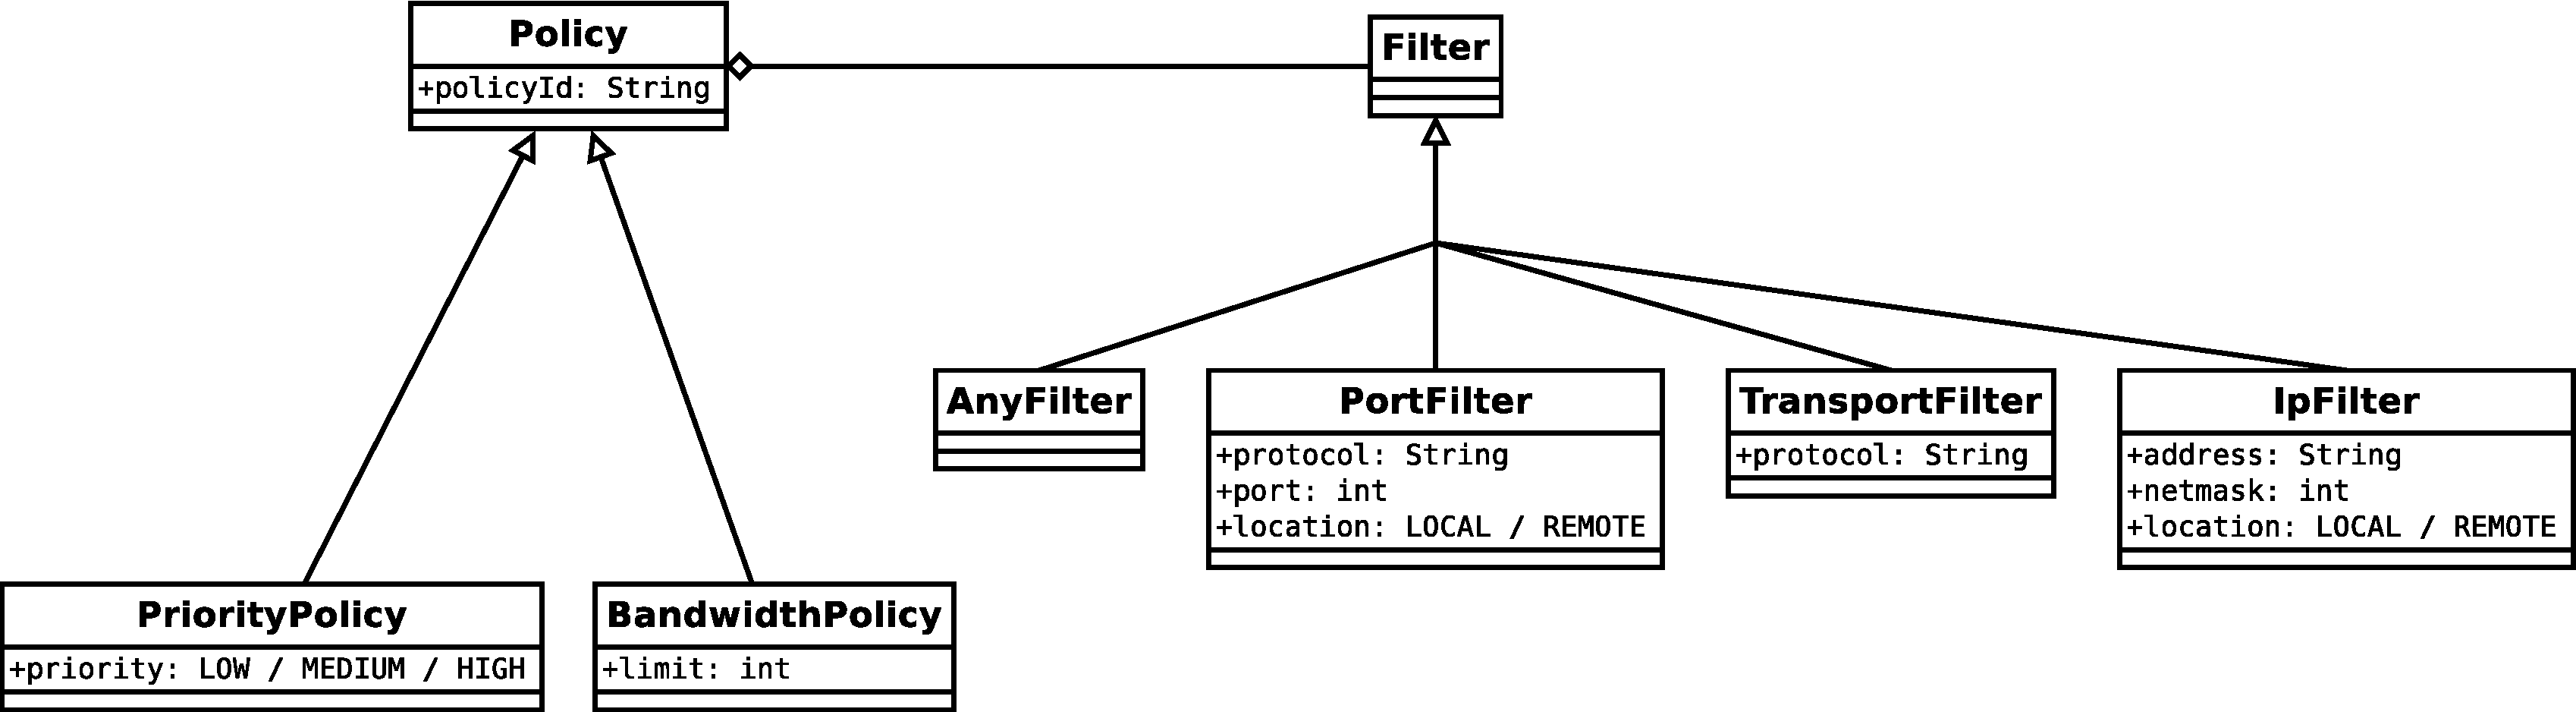
\includegraphics[width=0.7\textwidth]{img/architecture/om-policy.pdf}
                    \end{center}
                    \caption{Object model --- policies}
                  \end{figure}

          \end{itemize}


        \subsubsection{Modeling assignments}

          The assignment descriptor is used together with static data model to map entities to physical nodes. The
          descriptor is created automatically or by the user before instantiating the model as well as during the
          discovery stage when it is constructed by low-level components of the implemented system.

          The annotation part of the descriptor can be used to carry additional entity-specific properties that have to
          be passed between components. It can also be used to hold auxiliary data while performing internal
          transformations of the model.

          \begin{figure}[H]
            \begin{center}
              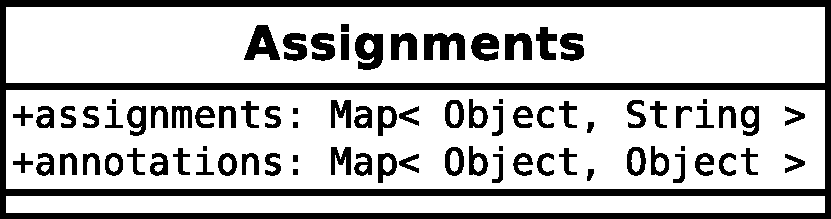
\includegraphics[scale=.5]{img/architecture/assignments.pdf}
            \end{center}

            \caption{Assignments}
          \end{figure}


        \subsubsection{Actions}

          When managing the topology, actions play crucial role --- they describe, for each element of the model, the
          operation that is going to be performed. Actions are assigned not globally for the model but on per-object
          basis --- the approach that introduces more flexibility and efficiency.

          There are three types actions designed. The object in the model can be created (ADD, as in instantiation
          phase), deleted (REM, typically performed after topology discovery) or modified (UPD, for entities that
          support on-line property adjustment).

          \begin{figure}[H]
            \begin{center}
              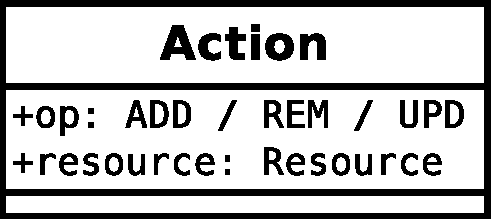
\includegraphics[scale=.5]{img/architecture/actions.pdf}
            \end{center}

            \caption{Actions}
          \end{figure}


      \subsection{System components and their responsibilities}

        The specific character of the system --- running in a distributed environment, moderate complexity --- requires
        proper architectural model. The model should allow to design the elements of the system to be highly cohesive
        and maintain coupling as loose as possible. Each component has its own well-defined role and exposes a set of
        operations to interact with others.

        The components presented in figure \ref{fig:arch:comp} reflect three main stages of operation shown in
        subsection \ref{sub:arch:hl}. Boundaries were introduced to make the partition even clearer. The following
        subsections describe the components in more detail and provide listings with most important methods of exposed
        interfaces.

        \begin{figure}[H]
          \begin{center}
            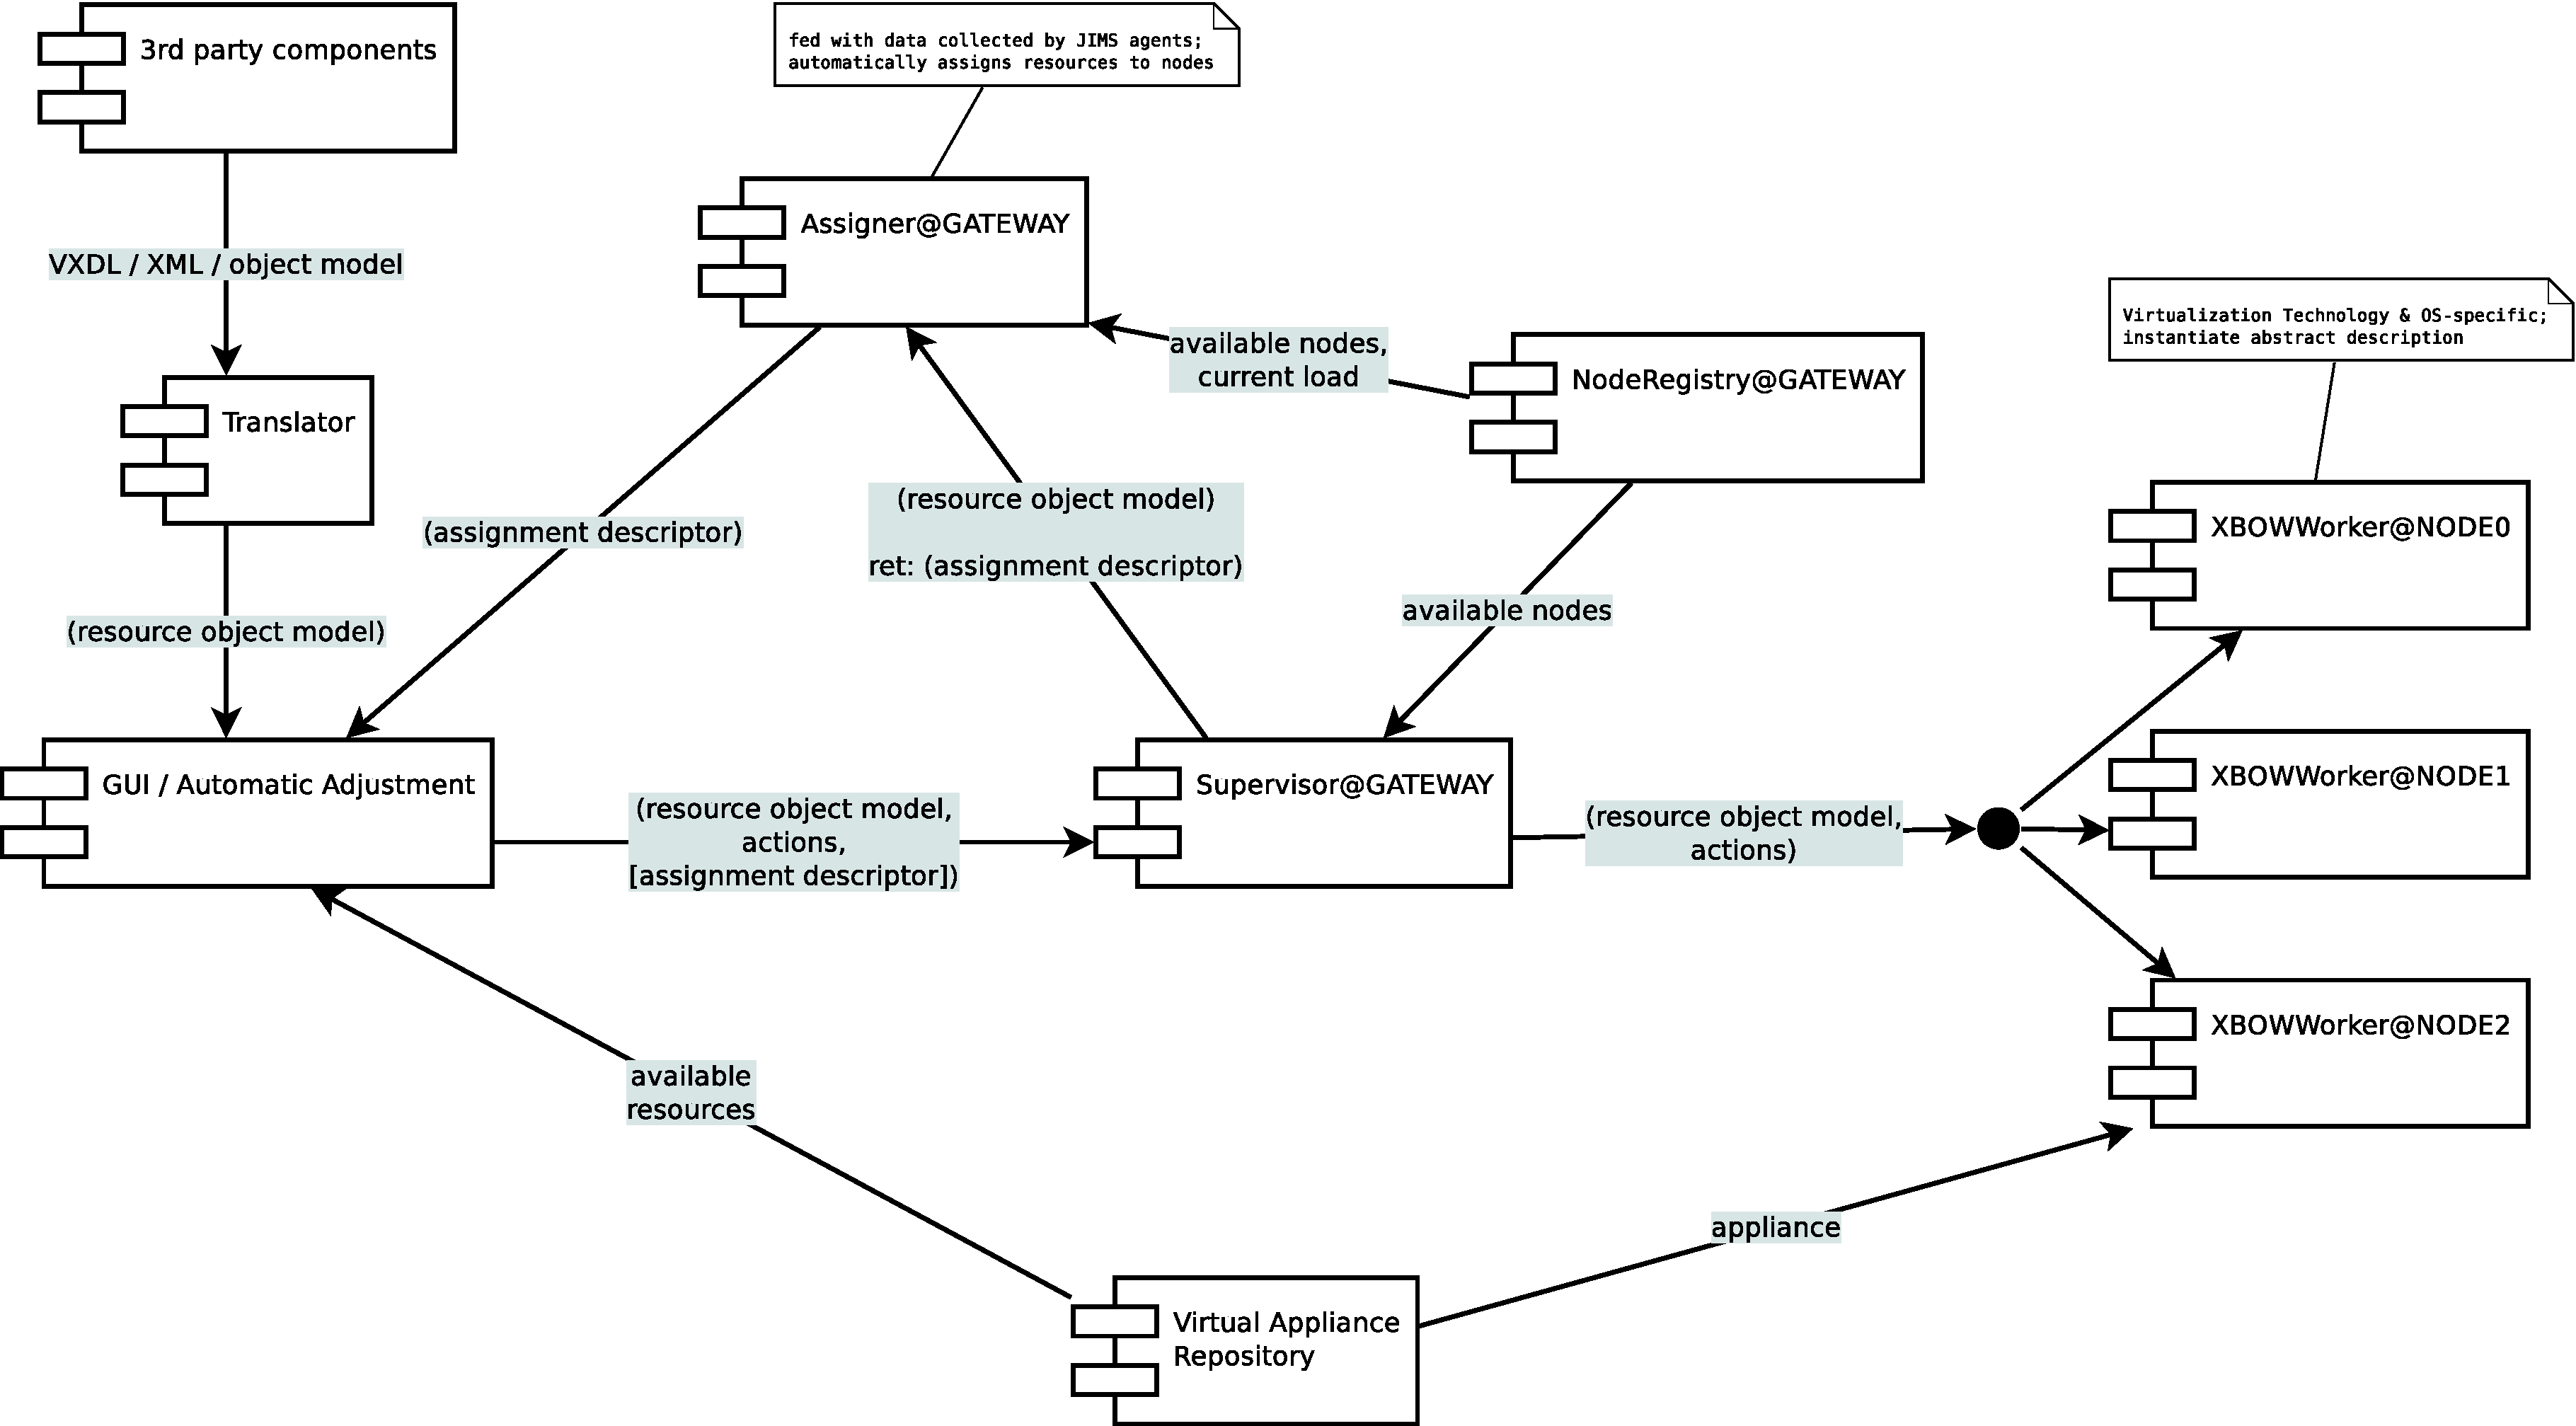
\includegraphics[width=\textwidth]{img/architecture/iaas-components.pdf}
          \end{center}

          \caption{Components of the system}
          \label{fig:arch:comp}
        \end{figure}


        \subsubsection{Virtual Appliance Repository}

          The main responsibility of Virtual Appliance Repository is to maintain the list of and provide access to
          virtual appliances created. It is used in two phases: the design phase to select appliances that are to be
          deployed, and instantiation phase to serve virtual appliance images. \\

          \noindent
          \begin{minipage}{\textwidth}
            \lstinputlisting[caption={Virtual Appliance Repository public interface},label={lst:arch:iface:repo},language=Java]{lst/arch-iface-repo.java}
          \end{minipage}
          

        \subsubsection{Assigner}

          The optional assigner module can handle entire assignment stage and make it fully automatic. To be able to do
          this, it has to be configured with a set of rules and has to continuously collect data about physical nodes
          load. If the assigner component is not present, logical model has to be assigned manually to available host
          machines.


        \subsubsection{Supervisor}

          Supervisor component manages all the worker nodes present in the system. Its responsibility is to perform
          preliminary model transformations (if needed --- for example, when using multiple host machines), divide the
          topology model according to the assignment rules and ask appropriate worker nodes to instantiate resulting
          parts.

          Supervisor delegates most of the work to worker nodes. Transactional operations can be provided at this level
          by extending the supervisor's behaviour to rollback after one of the worker nodes fails. \\

          \noindent
          \begin{minipage}{\textwidth}
            \lstinputlisting[caption={Supervisor public interface},label={lst:arch:iface:supervisor},language=Java]{lst/arch-iface-supervisor.java}
          \end{minipage}


        \subsubsection{Worker}

          Worker components perform all the low-level operations, including model to underlying entity mapping (and vice
          versa). Workers do not transform the model in any way --- all they do is provide well-defined rules for
          instantiation (including naming schemes) and discovery. Multiple workers are managed by the supervisor.

          Public interface of worker component is presented in listing \ref{lst:arch:iface:worker}. \\

          \noindent
          \begin{minipage}{\textwidth}
            \lstinputlisting[caption={Worker public interface},label={lst:arch:iface:worker},language=Java]{lst/arch-iface-worker.java}
          \end{minipage}


      \subsection{Main data flows and cooperation of the components}

        \subsubsection{Instantiation}

          There are three main stages identified when working with the topologies. There is a purely logical one that
          does not require any knowledge of the underlying environment --- the operations involve manipulating the
          domain model to create or update the virtual topology. There is an assignment stage which results in
          association between the model and physical resources. Finally, the actual deployment takes place in model
          instantiation stage --- logical elements are mapped to low-level ones after performing necessary
          transformations.

          Instantiation is the process of transforming a logical model to fully operational virtual network. There are
          three main stages that constitute the complete process:

          \begin{enumerate}

            \item Logical model definition

              This is the first stage the user is exposed to. The main task is to create a virtual network topology
              comprising logical networking components (belonging to Layer 2 and 3 of the \mbox{OSI/ISO} model) and
              virtual appliances --- specialized virtual machines. After the topology is created, IP addressing is
              provided and routing set up. Finally, Quality of Service policies are determined to classify and
              differentiate the traffic.

            \item Physical resource selection and assignment

              After the model is defined, it can be associated with underlying physical resources. There are two
              possible ways of performing the assignment --- it can be done manually with supplied utilities or special
              component can suggest optimal solution based on, for example, current workload and predefined set of
              rules. The latter approach is particularly useful when working with complex systems that should be able to
              adjust themselves automatically to balance the load.

            \item Model instantiation

              The final, entirely automatic, step is to map the logical model and assignments to actual components
              created on the host machines. This involves a series of transformations to adjust the model to
              capabilities of the underlying environment and satisfy other requirements like topology isolation.
                  
          \end{enumerate}

          \begin{figure}[H]

            \centering

            \begin{sequencediagram}

              \newthread{gui}{GUI}
              \newinst[2]{sup}{Supervisor}
              \newinst[4]{wrks}{Worker}
              \newinst[2]{var}{VA Repository}

              \begin{call}{gui}{getIds()}{var}{appliance IDs}
              \end{call}

              \begin{call}{gui}{instantiate(model)}{sup}{}
                \begin{callself}{sup}{transform(model)}{adjusted model}
                \end{callself}
                \begin{sdblock}{loop}{for each worker with model assigned}
                  \begin{call}{sup}{instantiate(parts of the model)}{wrks}{}
                    \begin{call}{wrks}{getAppliance(id)}{var}{virtual appliance}
                    \end{call}
                  \end{call}
                \end{sdblock}
              \end{call}
            
            \end{sequencediagram}

            \caption{Topology instantiation}
          
          \end{figure}

          % TODO co rozumiemy przez topologie? (topology=layout+qos)


        \subsubsection{Discovery}

          Instantiated topology, together with applied addressing, routing table entries and quality policies, can be
          discovered, i.e. object model that describes it can be recreated. The discovery process is an inverse of
          instantiation, it is composed of three phases (as shown in figure \ref{fig:arch:seqdis}):

          \begin{enumerate}

            \item The system resources are inspected by each of the Worker nodes and parts of the model together with
                  Assignment descriptors are created independently,

            \item partial results are collected and merged by the Supervisor. Redundant data is removed and necessary
                  transformations performed,

            \item complete model is passed further (e.g. to the GUI component).
          
          \end{enumerate}

          \begin{figure}[H]

            \centering

            \begin{sequencediagram}

              \newthread{gui}{GUI}
              \newinst[2]{sup}{Supervisor}
              \newinst[4]{wrk}{Worker}

              \begin{call}{gui}{discover()}{sup}{model}
                \begin{sdblock}{loop}{for each worker}
                  \begin{call}{sup}{discover()}{wrk}{parts of the model}
                  \end{call}
                \end{sdblock}
                \begin{callself}{sup}{merge(parts of the model)}{model}
                \end{callself}
              \end{call}
            
            \end{sequencediagram}

            \caption{Topology discovery}
            \label{fig:arch:seqdis}
          
          \end{figure}


        \subsubsection{Monitoring}

          Topology operation can be monitored with high degree of granularity. Single flows can be inspected to see the
          amount of data transferred. Historical data is also made available.

          The StatisticsGatherer component performs the translation between domain models, for example it is able to map
          Policy to corresponding Flow and retrieve traffic statistics. The operation in shown in figure
          \ref{fig:arch:seqmon}.

          \begin{figure}[H]

            \centering

            \begin{sequencediagram}

              \newthread{gui}{GUI}
              \newinst[2]{gat}{StatisticsGatherer}
              \newinst[2]{ent}{Entity object}

              \begin{call}{gui}{getStatistics()}{gat}{statistics}
                \begin{call}{gat}{getStatistics()}{ent}{statistics}
                \end{call}
              \end{call}
            
            \end{sequencediagram}

            \caption{Topology monitoring}
            \label{fig:arch:seqmon}
          
          \end{figure}


    \section*{Summary}

      % TODO napisac tu cos sensownego

      The chapter provided description and discussion of the system's architecture. The high-level layered design was
      presented and its advantages listed. Flexible and easily-expandable resources instrumentation layer was analyzed.
      The layer provides general-purpose abstractions over low-level system resources.  Finally, the topmost layer,
      virtual infrastructure management, used to build complex virtual network topologies was introduced.

      The design satisfies requirements the system has to meet and ensures easy expansion when necessary. Thanks to low
      coupling, new components can be integrated whenever additional functionality is needed. The created system can
      scale to support large topology models deployed on a number of physical host preserving small amount of time
      needed for instantiation process.


  \chapter{Implementation}
    
    \section*{Chapter overview}
	
      This chapter focuses mainly on implementational details, especially on most interesting aspects of our system.
		
      Section \ref{sec:impl:env} informs about implementational environment aspects like requested operating system,
      libraries presence or necessary programs to be build and installed. 
	  
	  Section \ref{sec:impl:module} concerns about implemented crossbow module for JIMS
	  
		\quad Subsection \ref{sec:impl:general} initially introduces to crossbow module requirements.

		\quad Subsection \ref{sec:impl:comp} describes in detail created components facilitating crossbow usage.
		
		\quad Subsection \ref{sec:impl:low} lists low level functions used in created system.

		\quad Subsection \ref{sec:impl:model} outlines domain model transformation details.
		
		\quad Subsection \ref{sec:impl:infrastructure} highlights created infrastructure allowing easy integrating with GUI.
		
		\quad Subsection \ref{sec:impl:persist} describes adopted approach to data persistance.
		
	  
	  Section \ref{sec:impl:gui} concerns about GUI application.
	  
	  Section \ref{sec:impl:verif} briefly highlights system verfication.
	
	  Section \ref{sec:impl:build} presents all necessary steps required for platform build completion.
	  
		


    \section{Implementation environment}
    \label{sec:impl:env}

      JIMS Extensions for Resource Monitoring and Management of Solaris 10 provides general architecture for monitoring
      and management applications written in Java. 

      JIMS architecture is generally based on JMX ( Java Management Extensions ) - technology for distributed resource
      management. These managed resources in JMX are represented by MBeans which are simple Java objects registered at
      MBean Server under specific ObjectName \cite{jims}.
    
      \begin{figure}[H]
        \begin{center}
          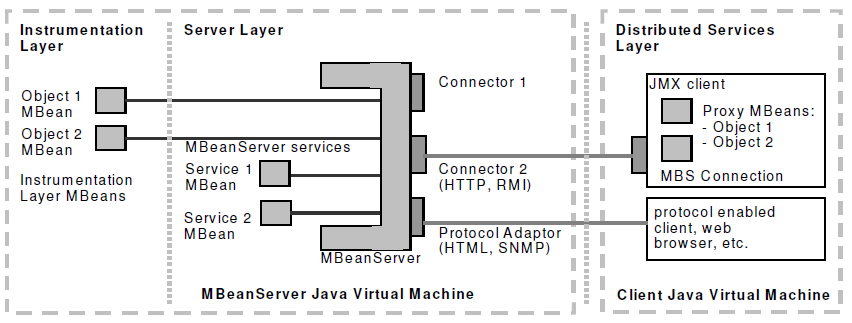
\includegraphics[width=0.9\textwidth]{img/jims/jmx.png}
        \end{center}
        \caption{JMX architecture \cite{jims}}
      \end{figure}
	
      JMX provides also services such as:

      \begin{itemize}
        \item Notifications,
        \item MLet (downloading dynamic modules).
      \end{itemize}
	
      JIMS (JMX based Infrastructure Monitoring System) supports monitoring and management under both Linux and Solaris
      platforms.  Due to Jims features such as: easy maintenance ( automatic modules downloading ), extensibility
      (possibility of adding additional modules) integrating with Jims newly developed module ( jims-crossbow ) was quite
      an easy task \cite{jims}.
    
      \begin{figure}[H]
        \begin{center}
          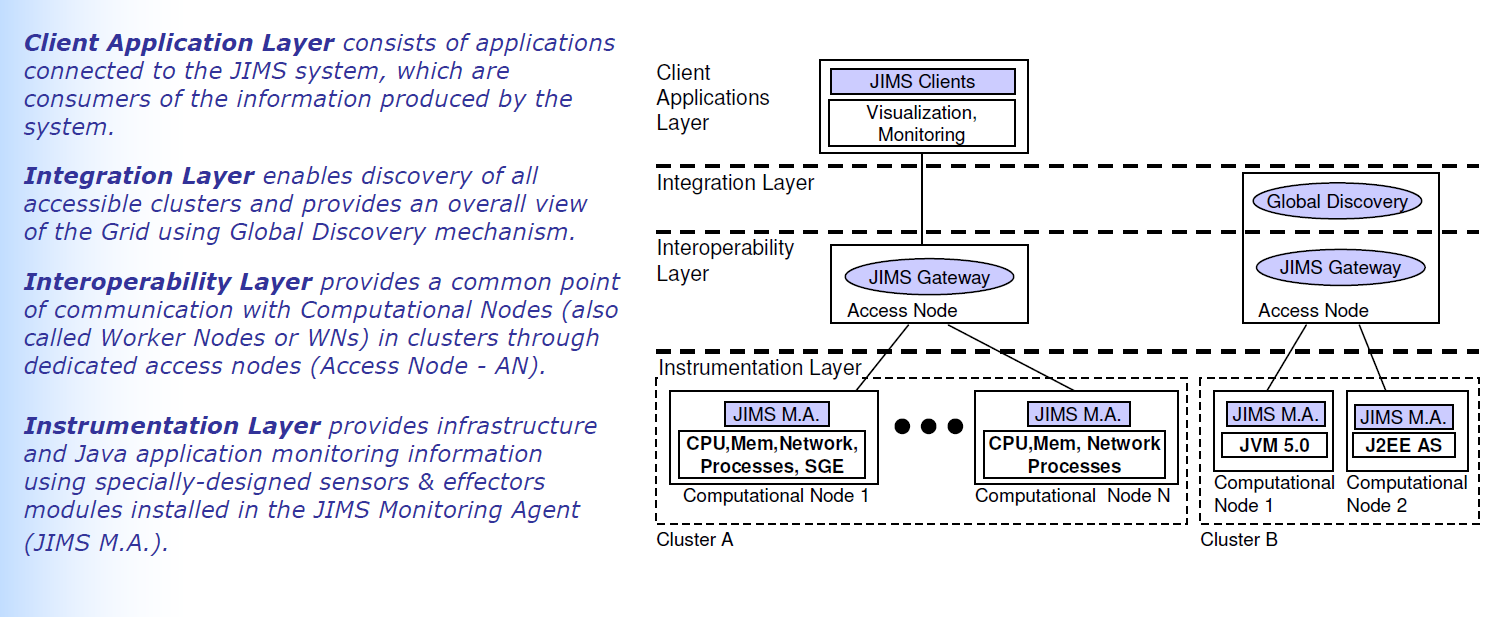
\includegraphics[width=0.9\textwidth]{img/jims/jims.png}
        \end{center}
        \caption{JIMS architecture \cite{jims}}
      \end{figure}
	 
      Jims services( MBeans ) enabling creating, reading and changing properties of zones and projects were extensively
      used in our system during deploying ( creating ) requested network structure. For more information about JIMS
      project please refer to the bibliography.	
    
      \medskip
	
      For the purpose of this paper two applications were implemented:
	
      \begin{itemize}
        \item Jims module for crossbow,
        \item GUI application.
      \end{itemize}
	  
	  \medskip
	
      In case of jims-crossbow module the implementation environment must consist:

      \begin{itemize}
        \item gcc compiler - for building jims-crossbow shared librarires,
        \item dladm, flowadm libraries.
      \end{itemize}
	
      The demand for crossbow libraries ( flowadm, dladm ) implicated that implementation environment must have been
      Solaris 11 or any other system supporting crossbow.
    
      GUI application was developed in java using swt and swing graphic libraries. Project was managed with maven and
      thanks to maven profiles feature can be build and run on operating systems like:

      \begin{itemize}
        \item Solaris,
        \item Linux x86,
        \item Windows x86.
      \end{itemize}

      SWT core libraries for these operating systems were provided in repository, so the only requirements is to have
      one of the already mentioned operating system and installed: Java se 1.6 and maven 2.x.
	  
	  \medskip
	  
	  Detailed description of these two appliactions are provided in two separate sections beneath. 
	  
	  \section{Crossbow module for Jims}
		\label{sec:impl:module}
	
		\subsection{General information}
			\label{sec:impl:general}
		
			To provide fully functionate system allowing all expected functionalities ( described in requirement analysys section )
			new module called \"jims-crossbow\" was implemented. Created module consists three projects:
			\begin{itemize}
				\item{Crossbow model components - performing crossbow like operations ( \textbf{jims/jims-crossbow/jims-crossbow-mbean} )}
				\item{Domain model transformation responsible for describing domain with actions 
					( described in separate section ) ( \textbf{jims/jims-crossbow/jims-crossbow-model} )}
				\item{Infrastructure project for high-level management ( \textbf{jims/jims-crossbow/jims-crossbow-infrastructure} )}
			\end{itemize}
		
		\subsection{Crossbow components implementation details}
			\label{sec:impl:comp}
	
		In terms of crossbow components, two kinds of them have been distinguished:

		\begin{itemize}
			\item Managers,
			\item Entities.
		\end{itemize}

		Managers basically provide operations for entity discovery and general management. The following managers have
		been created:

		\begin{itemize}
			\item VNicManager,
			\item EtherstubManager,
			\item FlowManager.
		\end{itemize}

		Another component type is entity which is basically equivalent of single crossbow entity like VNic, Etherstub.
		These entities appear as MBeans and are registered at MBean servers. Each bean contains basic information about
		entity like name, assigned properties and other attributes depending on their type. Operations for altering
		properties, parameters, ip address are provided as well. Three figures below depicts in detail each manager and
		their corresponding entity.

        \begin{figure}[H]
          \begin{center}
            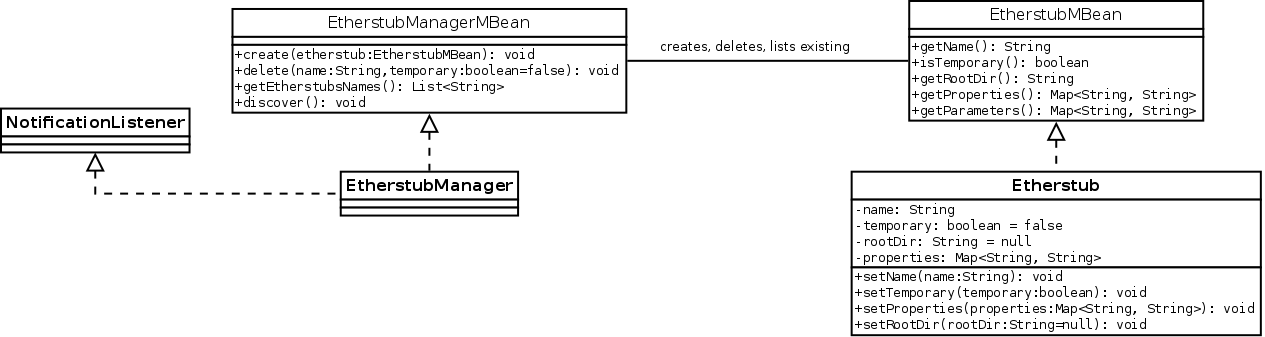
\includegraphics[width=1.2\textwidth, angle=90]{img/impl/etherstub.png}
          \end{center}
          \caption{Etherstub class diagram}
        \end{figure}        

        \begin{figure}[H]
          \begin{center}
            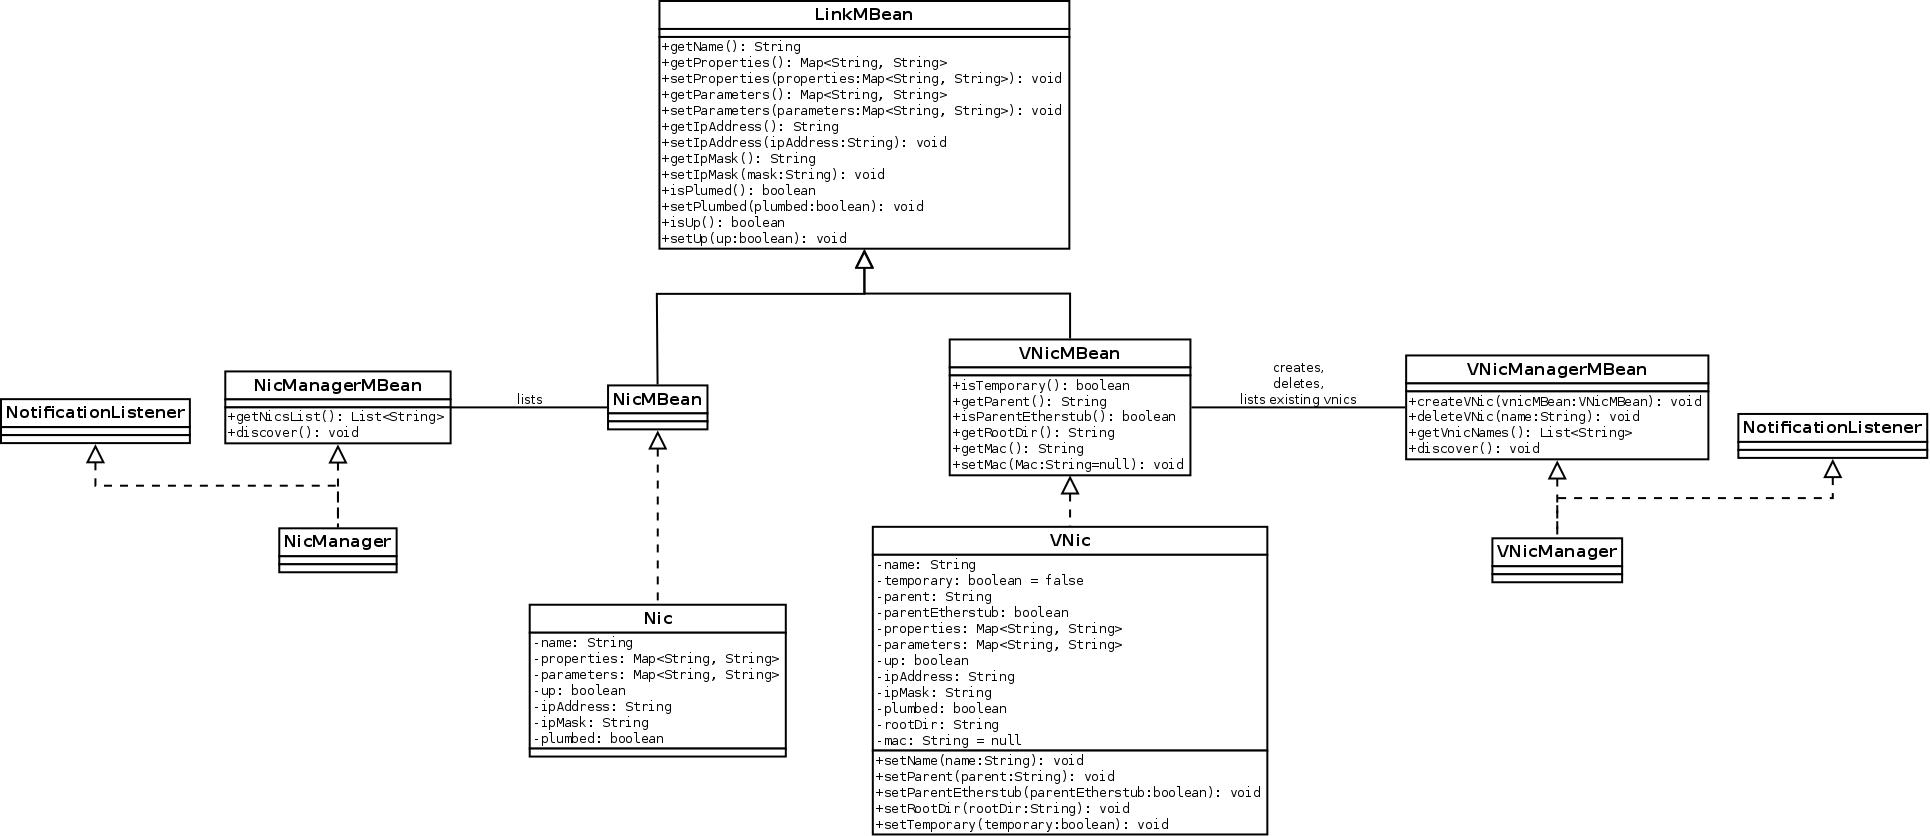
\includegraphics[width=1.2\textwidth, angle=90]{img/impl/link.png}
          \end{center}
          \caption{Link (VNic, Nic) class diagram}
        \end{figure}        

        \begin{figure}[H]
          \begin{center}
            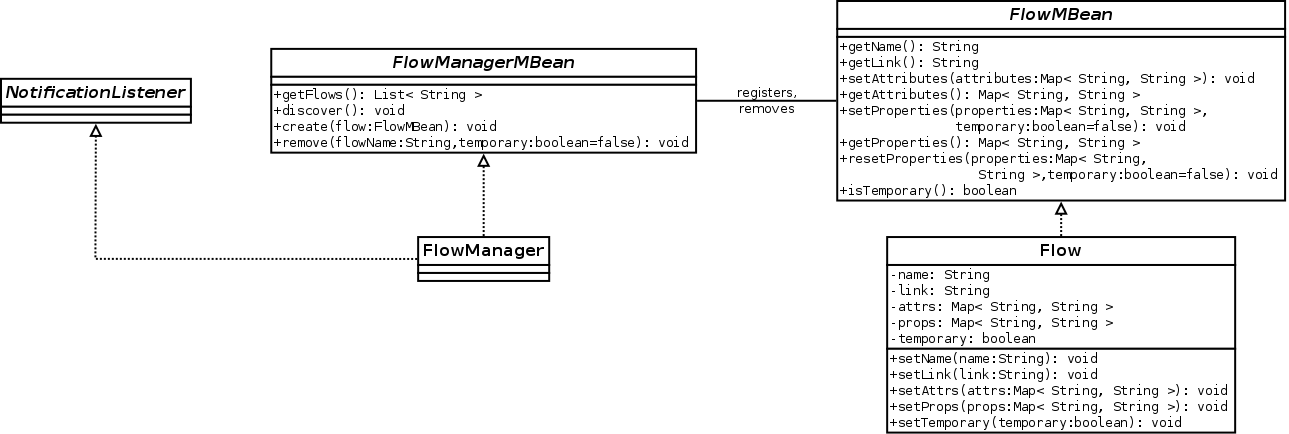
\includegraphics[width=1.2\textwidth, angle=90]{img/impl/flow.png}
          \end{center}
          \caption{Flow class diagram}
        \end{figure}        

		Due to the fact that managers and entities have been separated and that each entity is an individual MBean these
		entities can be accessed not only from java code but also be viewed and modified from jconsole.

		\begin{figure}[H]
			\begin{center}
			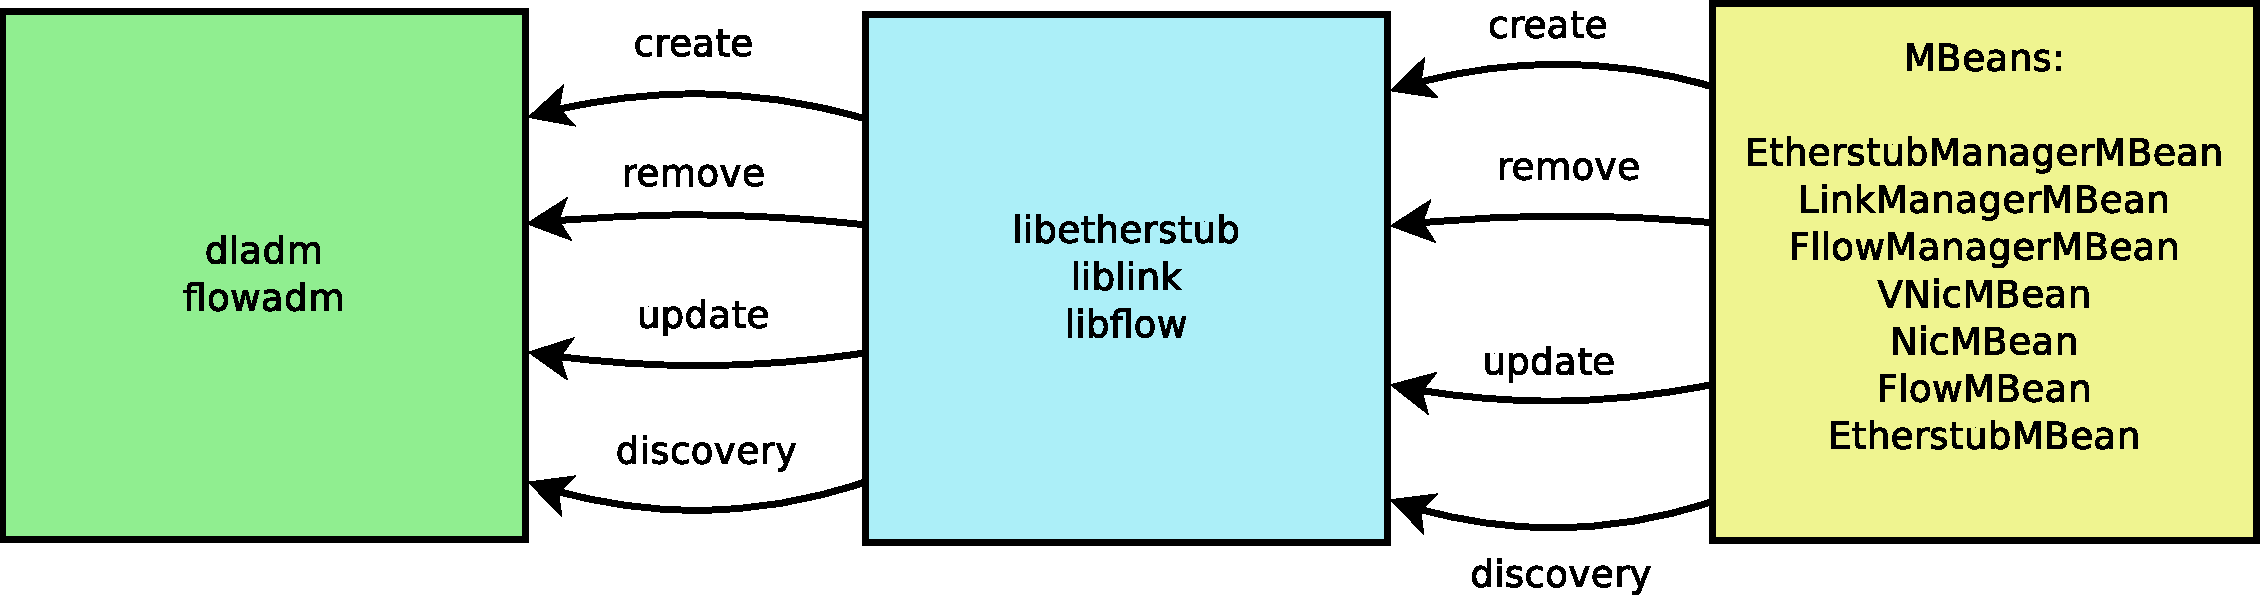
\includegraphics[width=0.9\textwidth]{img/impl/crossbowLibsDiagram.pdf}
			\end{center}
			\caption{Jims-crossbow components, shared libraries and crossbow native libraries relationship}
		\end{figure} 
		
		\subsection{Low-level functions access}
			\label{sec:impl:low}

			JIMS layered architecture implicated the demand for an approach towards accessing low-level funtions. In developed
			application these approaches were adjusted to existing conditions so that for accessing functions from shared
			libraries JNA (Java Native Access) was used and for doing more complex operations on low-level scripts were
			written and Java ProcessBuilder invoked. Created jims-crossbow module containes shared library allowing CRUD
			operations which subsequently are being accessed by JNA, whereas most of jims low-level access was done through
			running shell scripts. Although running scripts by ProcessBuilder is faster in some cases accessing native
			libraries through libraries like JNA or JNI gives more configurational advantage and does not require shell script
			writing ability.

			Listing \ref{lst:impl:low:jna} presents abbreviated example of JNA access to native libraries. \\
			Listing \ref{lst:impl:low:jna} presents abbreviated example of JNA access to native libraries. The corresponding
			native code in C language is shown in figure \ref{lst:impl:low:jnac}. \\
 	
	
			\noindent
				\begin{minipage}{\textwidth}
				\lstinputlisting[caption={Native library access with JNA (Java code)},label={lst:impl:low:jna},language=Java]{lst/impl-jna.java}
			\end{minipage}  

			\noindent
			\begin{minipage}{\textwidth}
				\lstinputlisting[caption={Native library access with JNA (Native code)},label={lst:impl:low:jnac},language=C]{lst/impl-jna.c}
			\end{minipage}


		\subsection{Domain model transformation details}
			\label{sec:impl:model}

		To allow conversion between GUI designed network structure (like in the figure below, more about GUI in separate subsection) to
                zones and crossbow entities on the server side new domain transformation model was proposed. 
      
		\begin{figure}[H]
			\begin{center}
			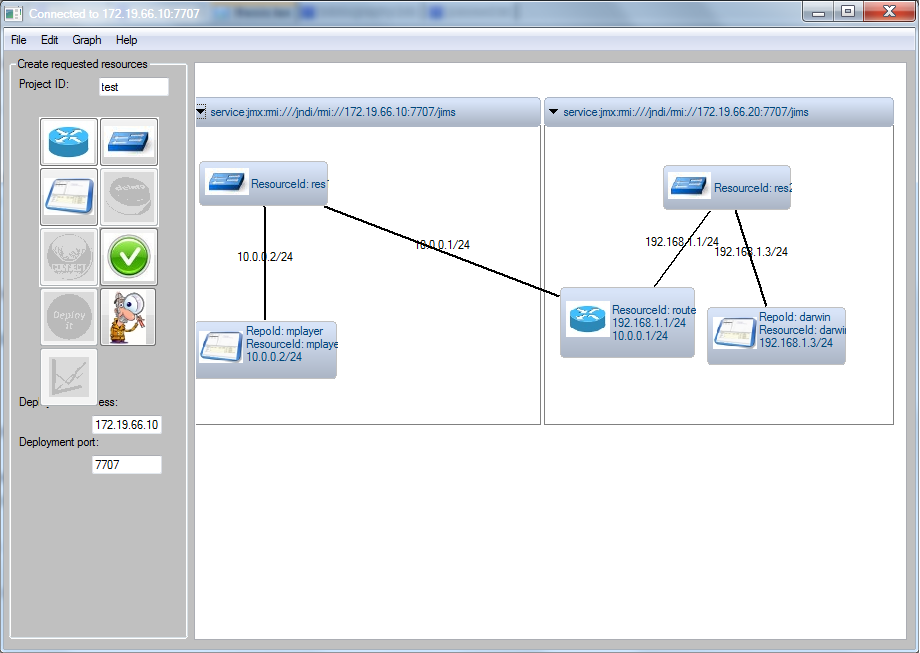
\includegraphics[width=1.0\textwidth]{img/impl/network_structure_example.png}
			\end{center}
			\caption{Example of a network structure to be converted to object model.}
		\end{figure} 

		In general four main class types were distinguished: Appliance, Switch, Interface, Policy.

		\medskip

		\textbf{Appliance} is an equivalent of a zone to be created from one of existing snapshots. Appliances could be
		also extended to Routers (with assigned static routes) which on the server side are seen as two appliances created
		under different etherstubs with routing tables modified and assigned interfaces enabling connectivity between
		appliances working under these two etherstubs. \\
		\textbf{Switch} is implied as crossbow etherstub. \\
		\textbf{Interface} is converted to VNic and assigned to created zones. \\
		\textbf{Policy} should be seen as a demand towards desired network traffic shape. Policy has assigned Flow Object
		with detailed values and flow type. These objects could be assigned directly to existing interfaces or exist as
		detached crossbow flows.

		\begin{figure}[H]
			\begin{center}
				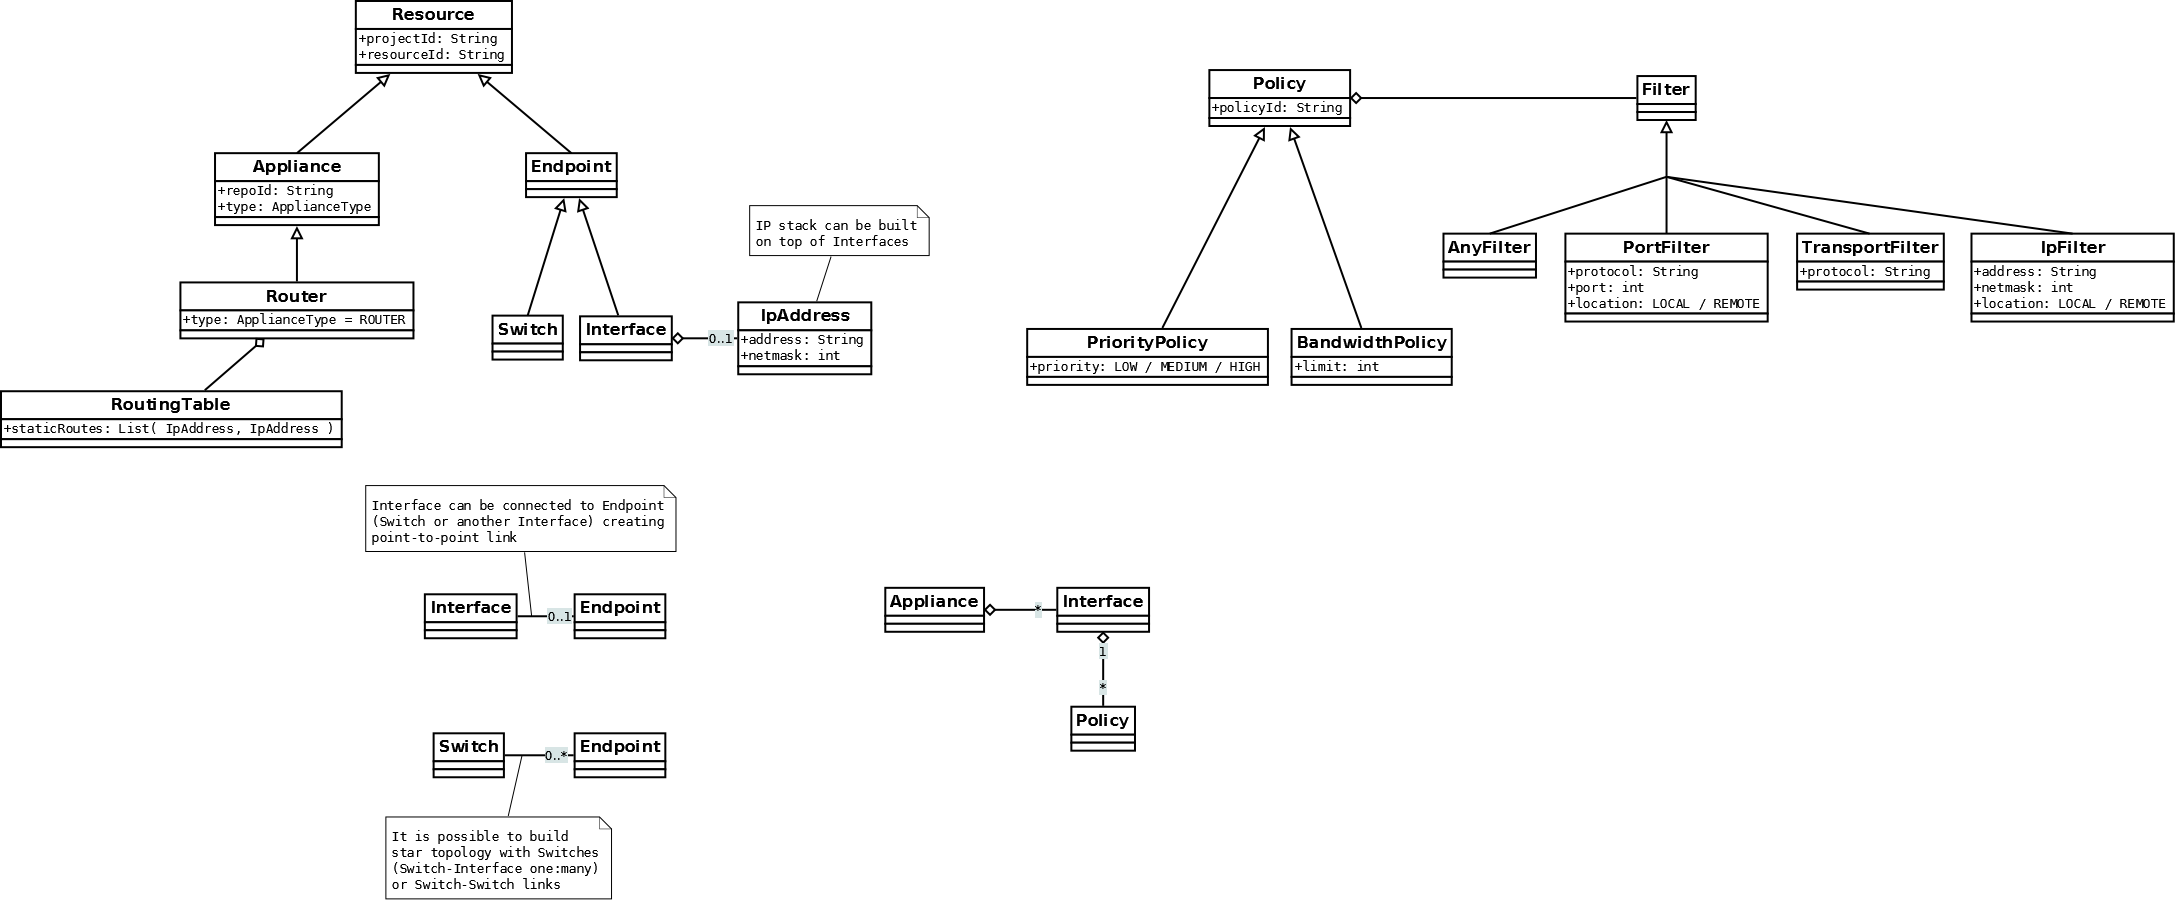
\includegraphics[width=1.2\textwidth, angle=90]{img/impl/resource-object-model.png}
			\end{center}
			\caption{Resource object transformation model}
		\end{figure}

		\begin{figure}[H]
			\begin{center}
				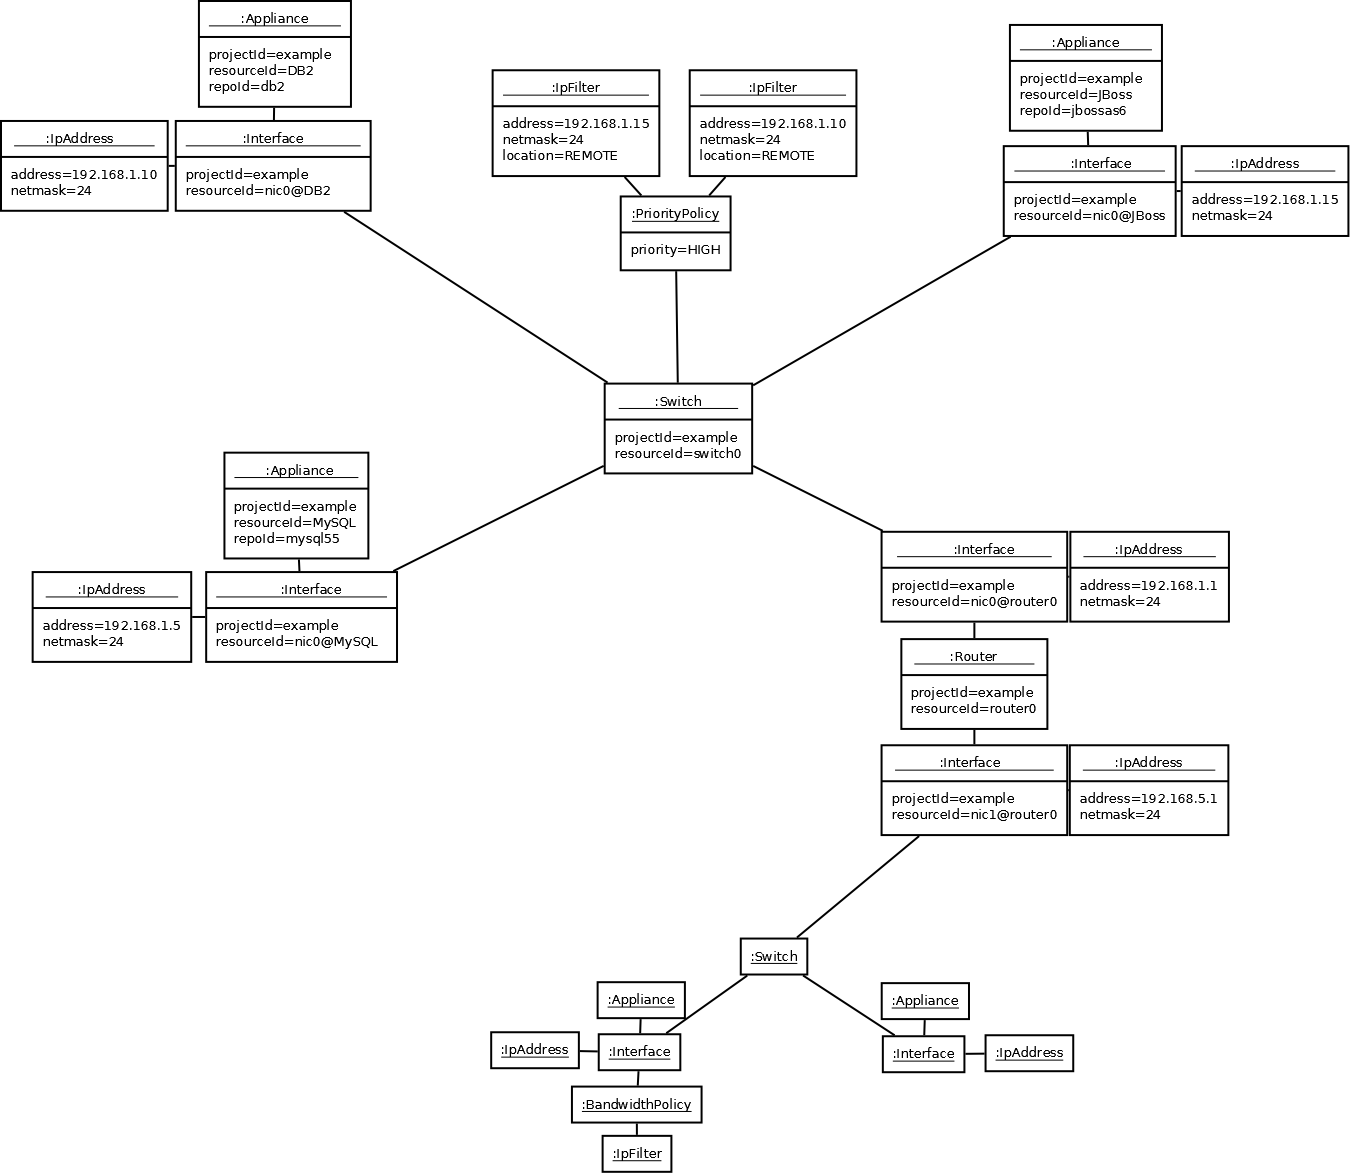
\includegraphics[width=0.9\textwidth]{img/impl/resource-object-model-example.png}
			\end{center}
			\caption{Resource object transformation model example}
		\end{figure}

		Created model was designed in order to comply requirement of multiple deployments so that only introduced changes
		were applied in already deployed project. Due to this issue to apply changes \textbf{instantiate(ObjectModel
		objModel, Actions actions)} method from \textbf{SupervisorMBean} must be invoked where ObjectModel class
		aggregates all domain model objects and Actions object encapsulates all actions to be done to every single domain
		model object. These actions would be:

		\begin{itemize}
			\item {ADD - adds new resource,}
			\item {REM - removes this resource,}
			\item {UPD - updates existing resource,}
			\item {NOOP - no changes are applied.}
		\end{itemize}
		
		\subsection{Crossbow infrastructure project}
			\label{sec:impl:infrastructure}
			
			As already mentioned whole system is based on JMX technology and externs existing JIMS project. All that
			provides separation layer. Operations provided by MBean's may invoked from created GUI, JConsole or even
			from own applications by just adapting to existing interfaces and object names. 
			
			Existing high-level MBean are described and discussed the table below:

			\begin{table}[ht]
				\caption{High-level management MBeans}
				\centering % used for centering table
				\begin{tabular}{llp{4cm}}
					\hline \hline
					Bean & ObjectName & Description \\
					\hline
					SupervisorMBean & \textbf{Crossbow:type=Supervisor} & Main Bean runs whole instantiation process ( distributes model to parts 
						and passes them to proper Worker \\
					\hline
					WorkerMBean & \textbf{Crossbow:type=XBowWorker} & Responsible for instantiating on  \newline
                                                this node given model with regard to specified  actions\\
					\hline
					RepoManagerMBean & \textbf{Crossbow:type=RepoManager} & Allows getting/setting path to projects placement, \newline returns all 
						existing projects from working path \\
					\hline
					FlowManagerMBean & \textbf{Crossbow:type=FlowManager} & Provides CRUD operations for Flows \\
					\hline
					EtherstubManagerMBean & \textbf{Crossbow:type=EtherstubManager} & Provides CRUD operations for etherstubs \\
					\hline
					VNicManagerMBean & \textbf{Crossbow:type=VNicManager} & Provides CRUD operations for VNics \\
					\hline
					VlanManagerMBean & \textbf{Crossbow:type=VlanManager} & co to robi? \\
					\hline
					StatisticGathererMBean & \textbf{Crossbow:type=StatisticsGatherer} & Provides statistics for \
						interface or flow from specified time period \\
					\hline
					CrossbowNotificationMBean & \textbf{Crossbow:type=CrossbowNotification} & Returns progress of deployment, \newline
						logs with major information \\
					\hline
				\end{tabular}
			\end{table}
			
		
		\subsection{Data persistance}
			\label{sec:impl:persist}

			Although created system does provide data persistance in databases or any other formats persistance is provided. 
			Persistance is provided on two levels: first is on GUI level where user may save created network structure that would
			be then serialized into file and second on the jims nodes. During creation, discovery, removing network elements precise
			naming conventions are preserved. Due to this convention whole network is persistent and does not require any additional 
			databases or files. Since generated names are complex manual modification or creation of elements is not recommended as 
			it is easy to make hard to find bugs. Created GUI is provided for this purposes.

			With regard to statistics flow statistics are gathered and managed by operating system whereas 
			VNic's traffic load is gathered starting from JIMS restart.
		
		\subsection{System verification}
			\label{sec:impl:verif}
		
			Complexity of created system implies necessity of preparing tools verifing correctness of the system. In order to achieve 
			this verification tests on each level of our system were prepared. Starting from ( low-level ) shared libraries, where unit tests
			for methods in \textbf{C} were implemented, through JMX level ( with mocks ) up to integration tests testing creating whole 
			network structure.
		
			Additionally verification on the GUI side of the system was provided where network to be created is verified in respect of 
			proper names, ip addresses, etc.

	\section{GUI application}
		\label{sec:impl:gui}
		
		Created GUI application facilitates usage of JIMS and newly implemented crossbow module for JIMS. Apart from project verification 
                performed in the pre-instantiation stage, GUI application is based on invocating JMX Bean's operation and presenting received responses.

		Implemented GUI application allows:
		\begin{itemize}
			\item{Connecting to jims-gateway,}
			\item{Creating, modifying and removing desired network structure with requested virtual appliances,}
			\item{Discovering already created projects,}
			\item{Detailed information about links and flows like bandwidth load presented in charts for requested \
				time periods,}
			\item{Automatic logging using ssh to selected ( already deployed ) nodes and opening GUI-type terminal.}
		\end{itemize}		

		\begin{figure}[H]
			\begin{center}
				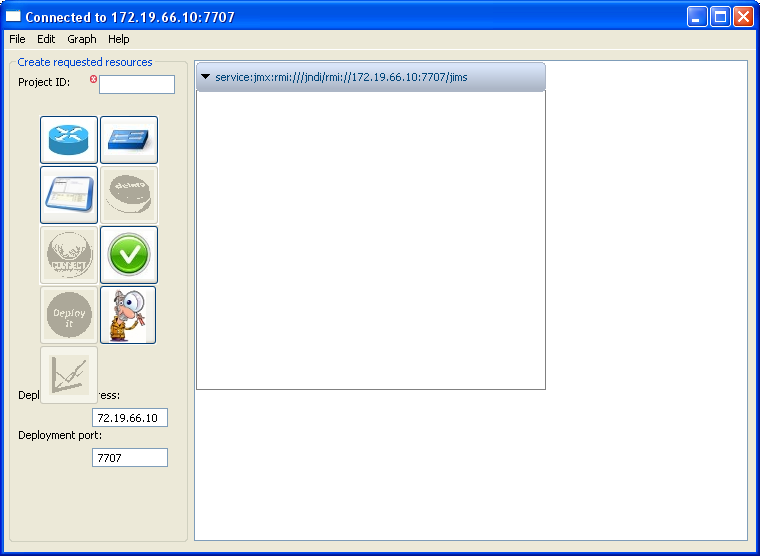
\includegraphics[width=1.0\textwidth]{img/impl/gui.png}
			\end{center}
			\caption{GUI application}
		\end{figure}

        \begin{figure}[H]

            \centering

            \begin{sequencediagram}

              \newthread{gui}{GUI}
              \newinst[2]{gtmt}{GraphToModelTranslator}
              \newinst{xbownotif}{CrossbowNotification}
              \newinst{progress}{ProgressShell}
              \newinst{sup}{Supervisor}

              \begin{call}{gui}{createActions(model, NetworkStructureHelper)}{gtmt}{Actions}
              \end{call}

              \begin{call}{gui}{resetTotal(int numberOfNodes)}{xbownotif}{}
              \end{call}

              \begin{call}{gui}{instantiate(model)}{sup}{}
              \end{call}

              \begin{call}{gui}{open()}{progress}{}
              \begin{sdblock}{loop}{while !deployed}
                \begin{call}{progress}{getProgress()}{xbownotif}{progress}
                \end{call}
                \begin{call}{progress}{getNewLogs()}{xbownotif}{logs}
                \end{call}
              \end{sdblock}
              \end{call}
            \end{sequencediagram}

            \caption{GUI side instantiation process}
          
          \end{figure}
		


    \section{Building and running the platform}
		\label{sec:impl:build}

      To build and run the platform the following prerequisites are required:

      \begin{itemize}
        \item Java SE 1.6, maven,
        \item jims sources downloaded,
        \item jims-crossbow module downloaded from \\ https://github.com/robertboczek/solaris\-crossbow/tree/master/code.
      \end{itemize}

      Afterwards JIMS project must be built. Detailed description of how to build JIMS is in \textbf{README} file
      located at the main catalog of jims sources. One of the most common problems are missing jars that unfortunately
      must be manually downloaded and installed in the local repository.

      Subsequently jims-crossbow module should be copied to the main folder containing jims and then build. The script
      \textbf{inst-crossbow-lib.sh} must be	later executed to copy shared libraries *.so files to /usr/lib folder.

      If everything went well another step is running JIMS:

      \begin{itemize}
        \item jims-gateway: .../jims-gateway/bin/jims-agent.sh [-b host\_address] start|stop|restart,
        \item jims-agent: .../jims-agent/bin/jims-agent.sh [-b host\_address] start|stop|restart.
      \end{itemize}

      On the main node just single jims-gateway should be run and on the rest nodes as many jims-agents as it is required. For more
      information about \textbf{jims} and its architecture please refer to bibliography.

      If jims-agent or jims-gateway did not started it is worth to see logs files, located respectively at
      target/.../jims-agent/var/jims/log/agent.log and target/.../jims-gateway/var/jims/log/agent.log
      It also recommended to have logs opened during JIMS start to see whether any exception was thrown (\textbf{tail
      -f target/.../jims\-gateway/var/jims/log/agent.log})

      JIMS has JMX-based architecture so each jims-agent and jims-gateway can be accessed through jconsole. In order to do that start 
      jconsole, select remote process and enter type: \\ \textbf{service:jmx:rmi:///jndi/rmi://address:port/jims} where \textbf{address} and 
      \textbf{port} is concrete address and port under which jims was started. \textbf{JConsole} allows browsing registered mbeans and 
      performing CRUD operations. Especially in case of the crossbow module it allows these operations as
      the figure below presents:

	  \begin{figure}[H]
        \begin{center}
            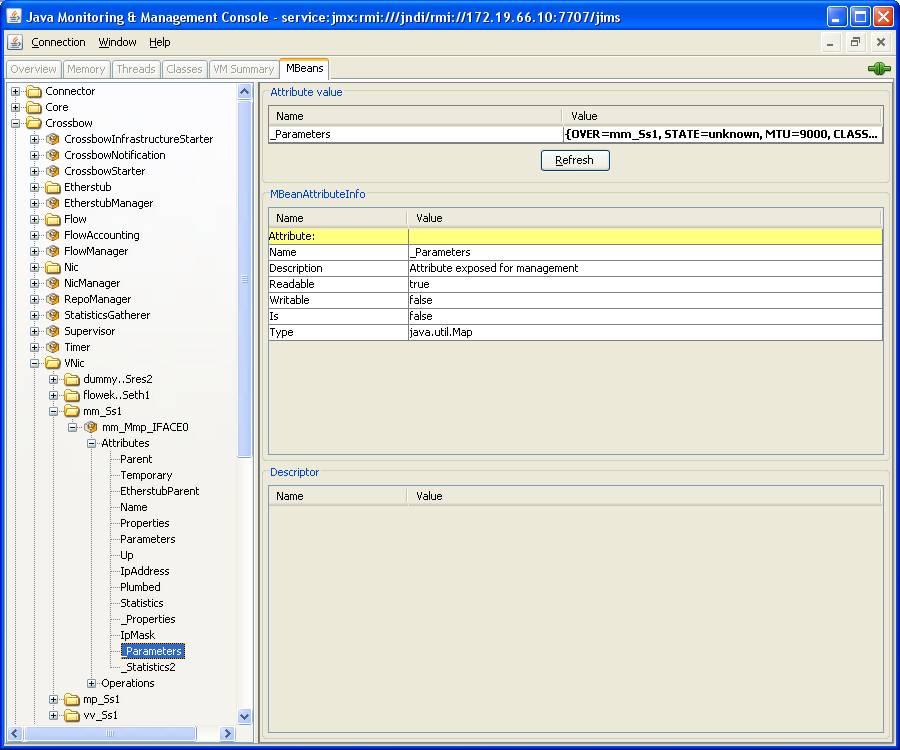
\includegraphics[width=1.0\textwidth]{img/impl/jconsole.png}
        \end{center}
        \caption{The Crossbow module registered MBeans example}
      \end{figure}
	  
	  Building GUI, which is located at \textbf{jims/jims-crossbow/jims-crossbow-gui}, requires just maven. Application may 
	  be imported to eclipse and then built and run or built from console using maven (\textbf{ mvn assembly:assembly })
	  and executed \textbf{java -cp target/jims-crossbow-gui-3.0.0-exe.jar org.jims.modules.crossbow.gui.Gui}


  \chapter{Case Study}

    The chapter describes the infrastructure that was built using the implemented system. Steps necessary to restore the
    configuration are listed and described. A number of tests were performed to evaluate the created system and
    topologies it allows to create. Resulting experimental data is presented and discussed.

    Section \ref{sec:uc:description} introduces the overall view of the topology that was created. Main components are
    described and QoS requirements are discussed in more detail. Types of service are presented and appropriate
    network-level policies described. The policies are assigned to network components.

    Section \ref{sec:uc:prep} describes the stages needed to set up the topology. The steps include virtual appliance
    creation and publication, topology design, determining the quality policy and instantiation. Domain model of the
    designed topology and resulting low-level entities are listed.

    Section \ref{sec:uc:operation} presents the results of experiments performed to verify requirements the system has
    to meet. The section focuses on Quality of Service-related aspects --- it verifies definition, management and
    operation of the policies.

    Section \ref{sec:uc:enhance} lists the advantages of using the proposed system and approach to create, manage and
    monitor QoS-aware virtual topologies. Aspects particularly helpful when preparing the case study are highlighted.


    \section{Scenario description}
    \label{sec:uc:description}

      The test case is inspired by multimedia systems. The problems of quality-aware transmission arise naturally
      in multimedia-oriented networks. Moreover, there are easily-identifiable classes of traffic with non-uniform
      quality requirements. This characteristics make multimedia networks a reasonable choice when considering tests
      focused on quality requirements verification.
      
      Also, complex topologies are built to enable multimedia transmission. The components that comprise these networks
      include, among others, specialized media servers, routers and client machines. This variety allows to demonstrate
      the usefulness of the created systems in the process of designing such topologies.


      \subsection{Types of service}
      
        As already stated, there are classes of traffic (or service types) that, by their nature, require different
        amounts of available resources (such as bandwidth, processing priority, etc.). The types of multimedia services
        map directly to QoS policies required. Table \ref{tab:uc:qos} shows the mapping.

        \begin{table}[H]
          \begin{center}
            \begin{tabular}{|c|c|c|}
              \hline
              service type        & bandwidth & delay tolerance \\
              \hline \hline
              real-time streaming & high      & low \\
              \hline
              video on demand     & high      & high  \\
              \hline
            \end{tabular}
          \end{center}

          % TODO uzupelnic; czy zrodlo?

          \caption{Multimedia network traffic and its requirements}
          \label{tab:uc:qos}
        \end{table}

        The most demanding type of multimedia data is undoubtedly real-time streaming. The high priority data has to be
        favoured in order to provide desired level of quality --- precedence when accessing transport media and
        low-jitter transfer. This allows for low-delay streaming with small input data buffers on the client side.

        Video on demand data is of less priority. It is assumed that the user is not going to utilize the data as it is
        being downloaded. This assumption loosens the transmission requirements and allows to treat VOD traffic as
        medium-priority or even best-effort data (no CIR).


      \subsection{Topology overview}

        The network topology built is an attempt to model simple yet real environment used to transmit multimedia data.
        There is a streaming server without user differentiation mechanisms (with respect to quality of transmission)
        and an HTTP server handling VOD requests. The clients connect to the streaming server and start streaming
        sessions. They can also download video served by the HTTP daemon.

        Client and server components are placed in different subnetworks that, in turn, are connected with a QoS-aware
        router which provides one more level the policies can be defined at. Rules defined for the router's interfaces
        specify fine-grained policies for clients in subnetworks in addition to the ones defined at the server level.

        Taking this approach, it is easy to enable QoS-aware networking leveraging relatively simple applications. The
        aspects of choosing server and client implementations and providing quality of service become orthogonal and the
        whole design remains clear and maintainable. Figure \ref{fig:cs:scenario} presents an overview of the network
        structure and client configuration.
      
        \begin{figure}[H]
          \begin{center}
            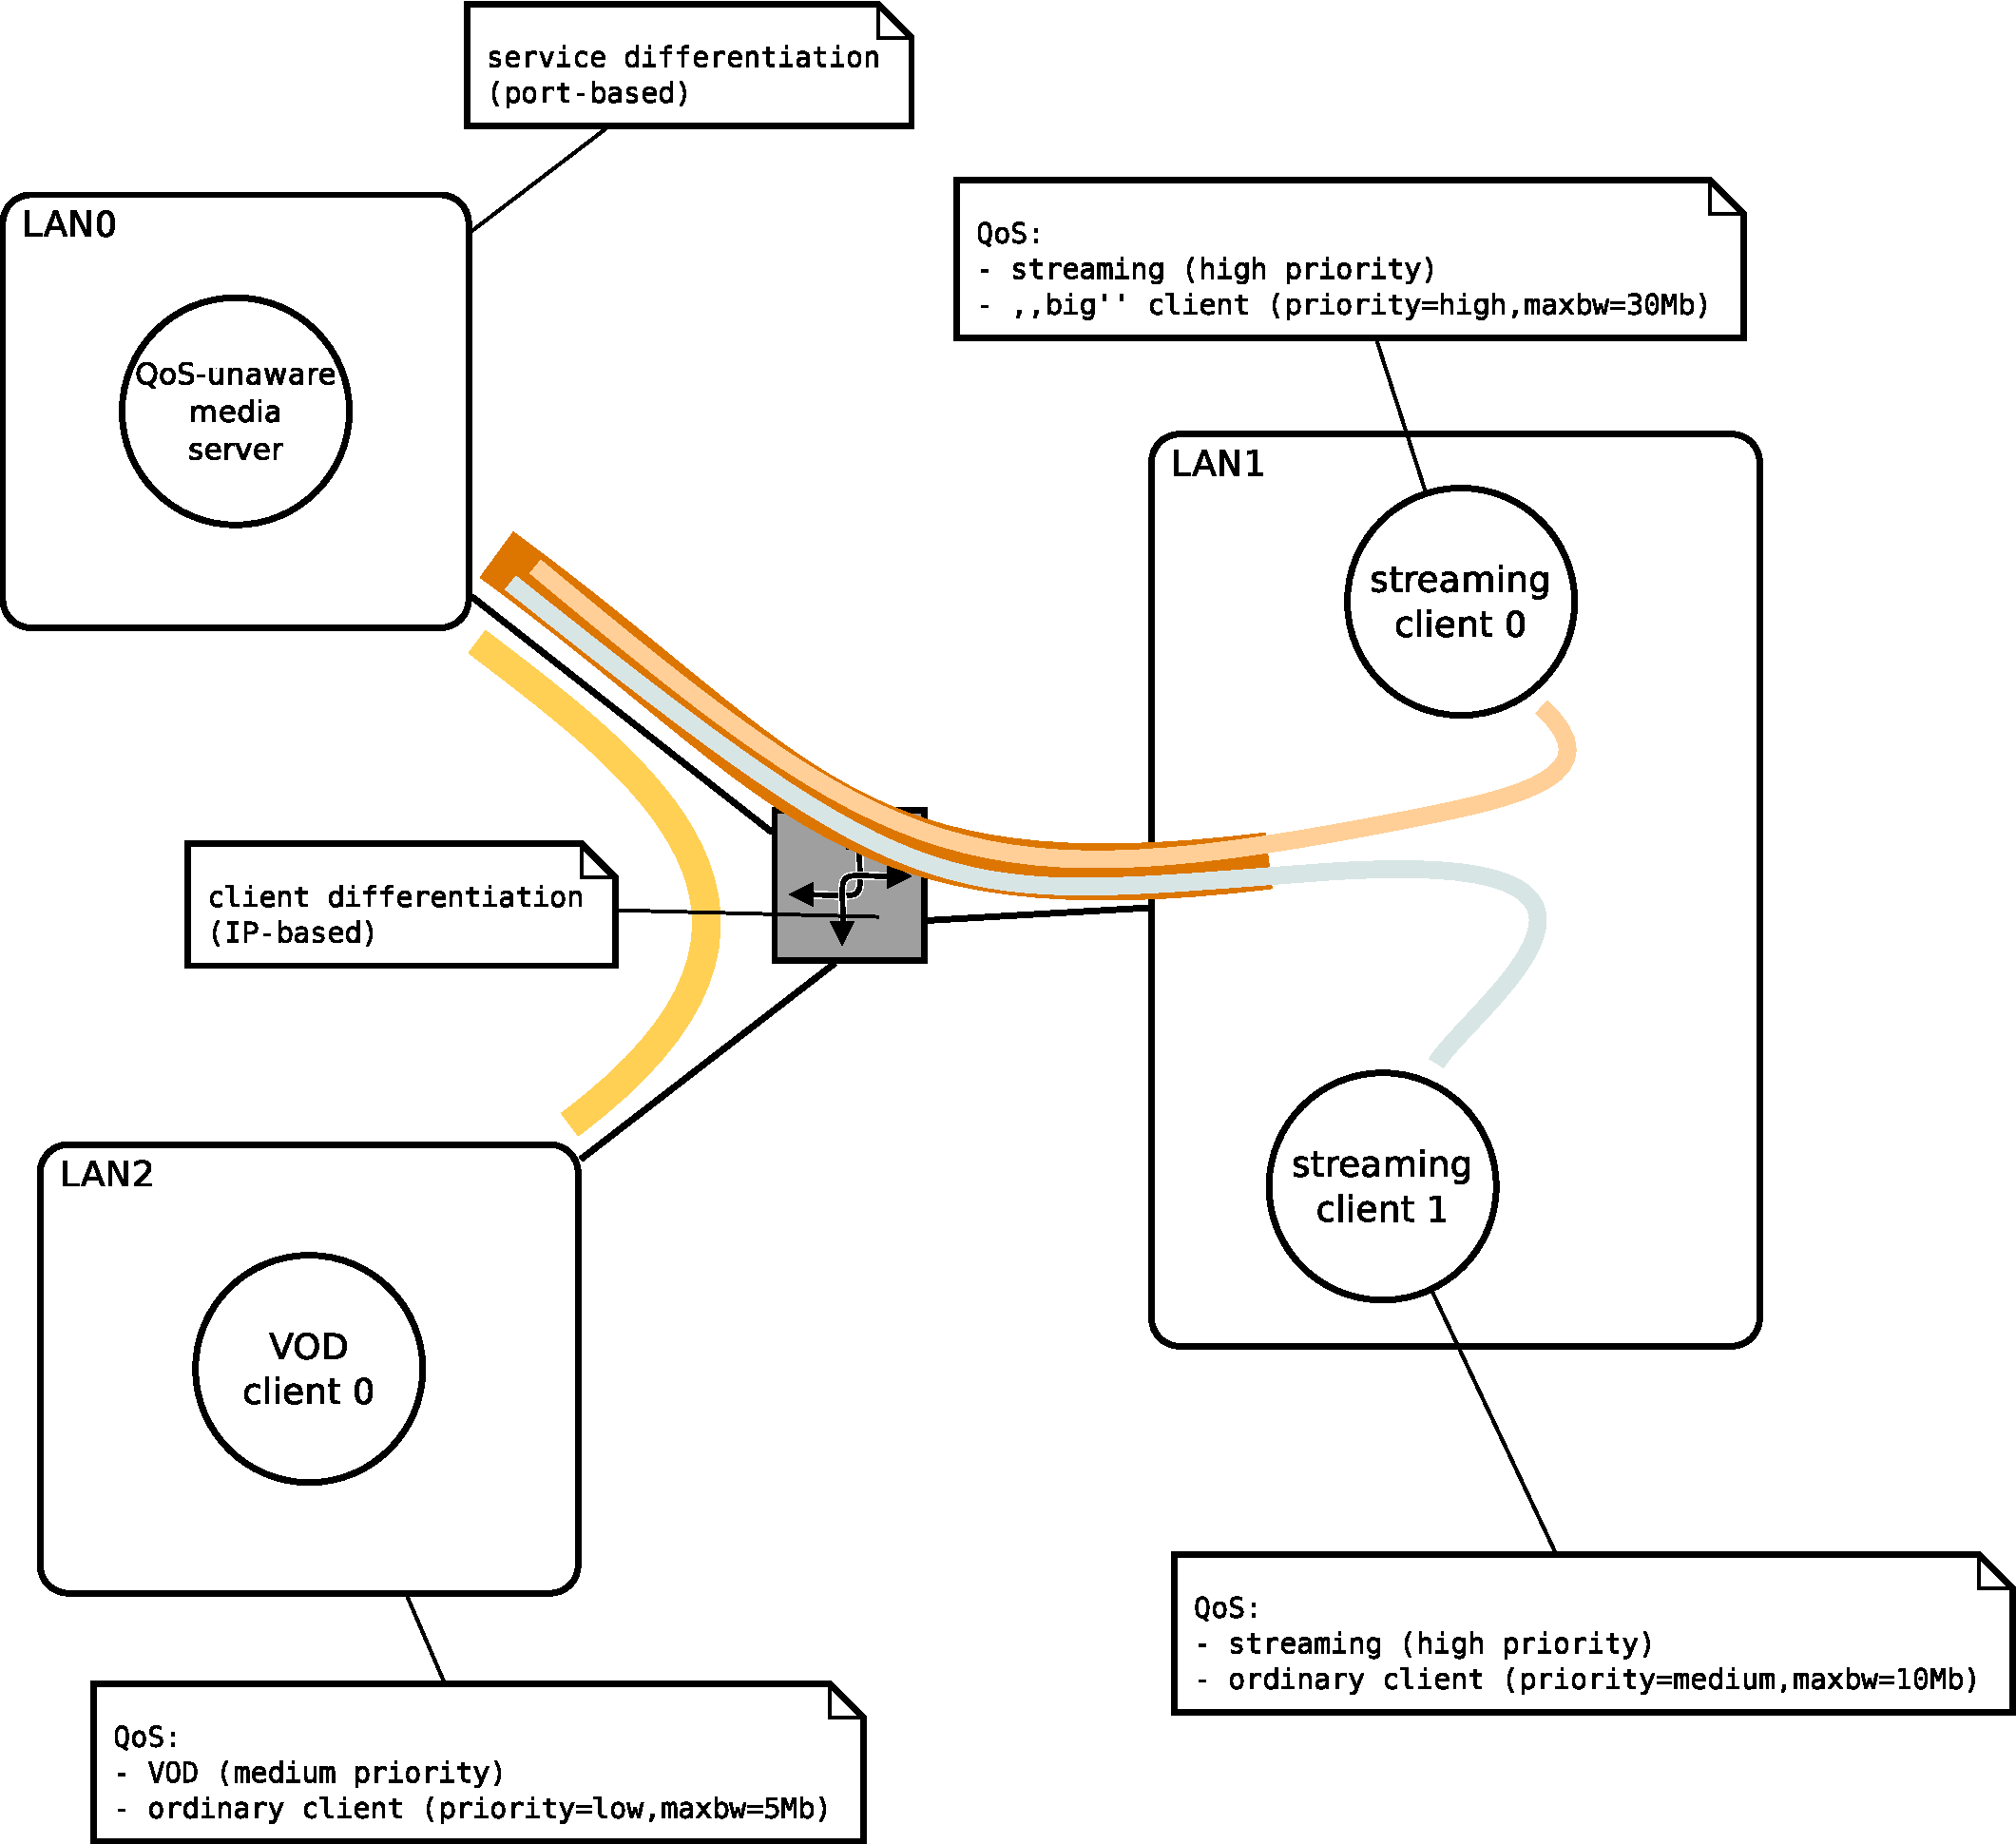
\includegraphics[width=0.8\textwidth]{img/test-case/diagram.pdf}
          \end{center}

          \caption{High-level view of the created topology}
          \label{fig:cs:scenario}
        \end{figure}
      

      \subsection{Service and client differentiation}
      \label{sub:uc:diff}

        The traffic is classified based on two properties: type of service (RTP, HTTP) and recipient address. Three
        traffic classes are distinguished with respect to service type:

        \begin{itemize}

          \item high priority RTP streaming

                UDP traffic with source ports 6970 and 6971, used by streaming client 0
                and streaming client 1 in LAN1 subnetwork,

          \item low priority Video On Demand
          
                TCP traffic with source port 80, used by the VOD client 0,

          \item medium priority ordinary traffic
          
                all the other data.

        \end{itemize}

        Furthermore, the streaming clients inside the LAN1 subnetwork are assigned different priority values. Client 0 is
        favoured and has high priority for RTP data, whereas client 1 is assigned low priority. Client 0 in LAN2
        is not assigned any priority explicitly.


    \section{Preparation of the environment}
    \label{sec:uc:prep}

      General steps while building the environment are: virtual appliance preparation, topology design and
      instantiation. Virtual appliances are created manually and published in an NFS repository. Then, they are used as
      building blocks when designing the network. Finally, the virtual infrastructure is instantiated, i.e. all the
      underlying low-level components, like zones, etherstubs, VNICs and flows, are created.


      \subsection{Virtual appliances}
      \label{ssub:case:prep:va}

        Listing \ref{lst:uc:prep:create} shows the initial steps when creating new zones. In this case, the zone is
        called \texttt{mplayer} and it contains a streaming client. At first, new ZFS pool is created to host the zone's
        filesystem, then basic configuration is performed and the zone is installed. \\

        \noindent
        \begin{minipage}{\textwidth}
          \lstinputlisting[caption={New zone creation},label={lst:uc:prep:create}]{lst/uc-create.sh}
        \end{minipage}

        \noindent
        It may be necessary to modify \texttt{/etc/shadow} file as in listing \ref{lst:uc:prep:sed} to be able to access
        the zone with \texttt{zlogin}. \\

        \noindent
        \begin{minipage}{\textwidth}
          \lstinputlisting[caption={\texttt{/etc/shadow} file adjustment},label={lst:uc:prep:sed}]{lst/uc-sed.sh}
        \end{minipage}

        \noindent
        After installation the zone can be booted and used after logging (listing \ref{lst:uc:prep:boot}). \\

        \noindent
        \begin{minipage}{\textwidth}
          \lstinputlisting[caption={Booting and logging into a zone},label={lst:uc:prep:boot}]{lst/uc-boot.sh}
        \end{minipage}

        \noindent
        All the required software should be installed now. When the zone is prepared, a ZFS snapshot can be taken and
        transferred to the repository (listing \ref{lst:uc:prep:snap}). \\

        \noindent
        \begin{minipage}{\textwidth}
          \lstinputlisting[caption={Publishing a snapshot in NFS repository},label={lst:uc:prep:snap}]{lst/uc-snap.sh}
        \end{minipage}


      \subsection{Topology instantiation}
      \label{ssub:}

        After all necessary virtual appliances have been created and stored in the repository, network topology can be
        designed and instantiated. Following steps comprise the whole process:

        \begin{enumerate}
          \item selection of virtual appliance templates from the repository,
          \item designation of physical machine(s) to host the topology,
          \item appliance-to-host assignment,
          \item enabling network connection between nodes, addressing, routing setup,
          \item defining QoS policies.
        \end{enumerate}

        The topology consists of router (forwards IP packets between its directly-attached interfaces), server (with
        Darwin Streaming Server and thttpd HTTP server installed) and client appliances (mplayer compiled with RTP
        streaming support enabled). All the appliances are instantiated on a single physical host.

        There are three subnetworks:

        \begin{itemize}
          \item 1.1.1.0/24 contains only the server appliance (addressed 1.1.1.2),
          \item 2.2.2.0/24 with one VOD client (addressed 2.2.2.2),
          \item 3.3.3.0/24 with two streaming clients (addressed 3.3.3.2 and 3.3.3.3).
        \end{itemize}

        The router appliance, with three interfaces (addressed 1.1.1.1, 2.2.2.1 and 3.3.3.1) links the subnetworks and
        provides network-level connectivity. Each of the appliances has additional entries in its routing table.

        Quality of Service assurance is composed of two main stages:

        \begin{itemize}
          \item bandwidth of the links used to stream and download media is limited to 8Mbps (mainly to make the
                testing process easier),
          \item traffic is divided into classes and policies are assigned to the classes.
        \end{itemize}

        Service differentiation is based on local port numbers and users are differentiated with respect to their
        network addresses. To achieve this, PortFilter and IpFilter are applied. PortFilter specifies a triple
        \mbox{(port number, location, protocol)} --- the example for RTP is \mbox{(6970, LOCAL, UDP)}. IpFilter
        specifies a triple \mbox{(IP address, netmask, location)} --- the example for a client in 1.1.1.0/24 subnetwork
        is \mbox{(1.1.1.2, 24, REMOTE)}.

        Relative bandwidth assignment is achieved with priorities. The PriorityPolicy instances determining traffic
        priority (LOW, MEDIUM, HIGH) have to be applied to specific interfaces.

        Figure \ref{fig:cs:topo} presents the complete topology built with domain model elements. It includes virtual
        appliances (:Machine, :Router), connectivity (:Interface, :IpAddress, :Switch), policies (:PriorityPolicy,
        :BandwidthPolicy) and filters (:PortFilter, :IpFilter).

        \begin{figure}[H]
          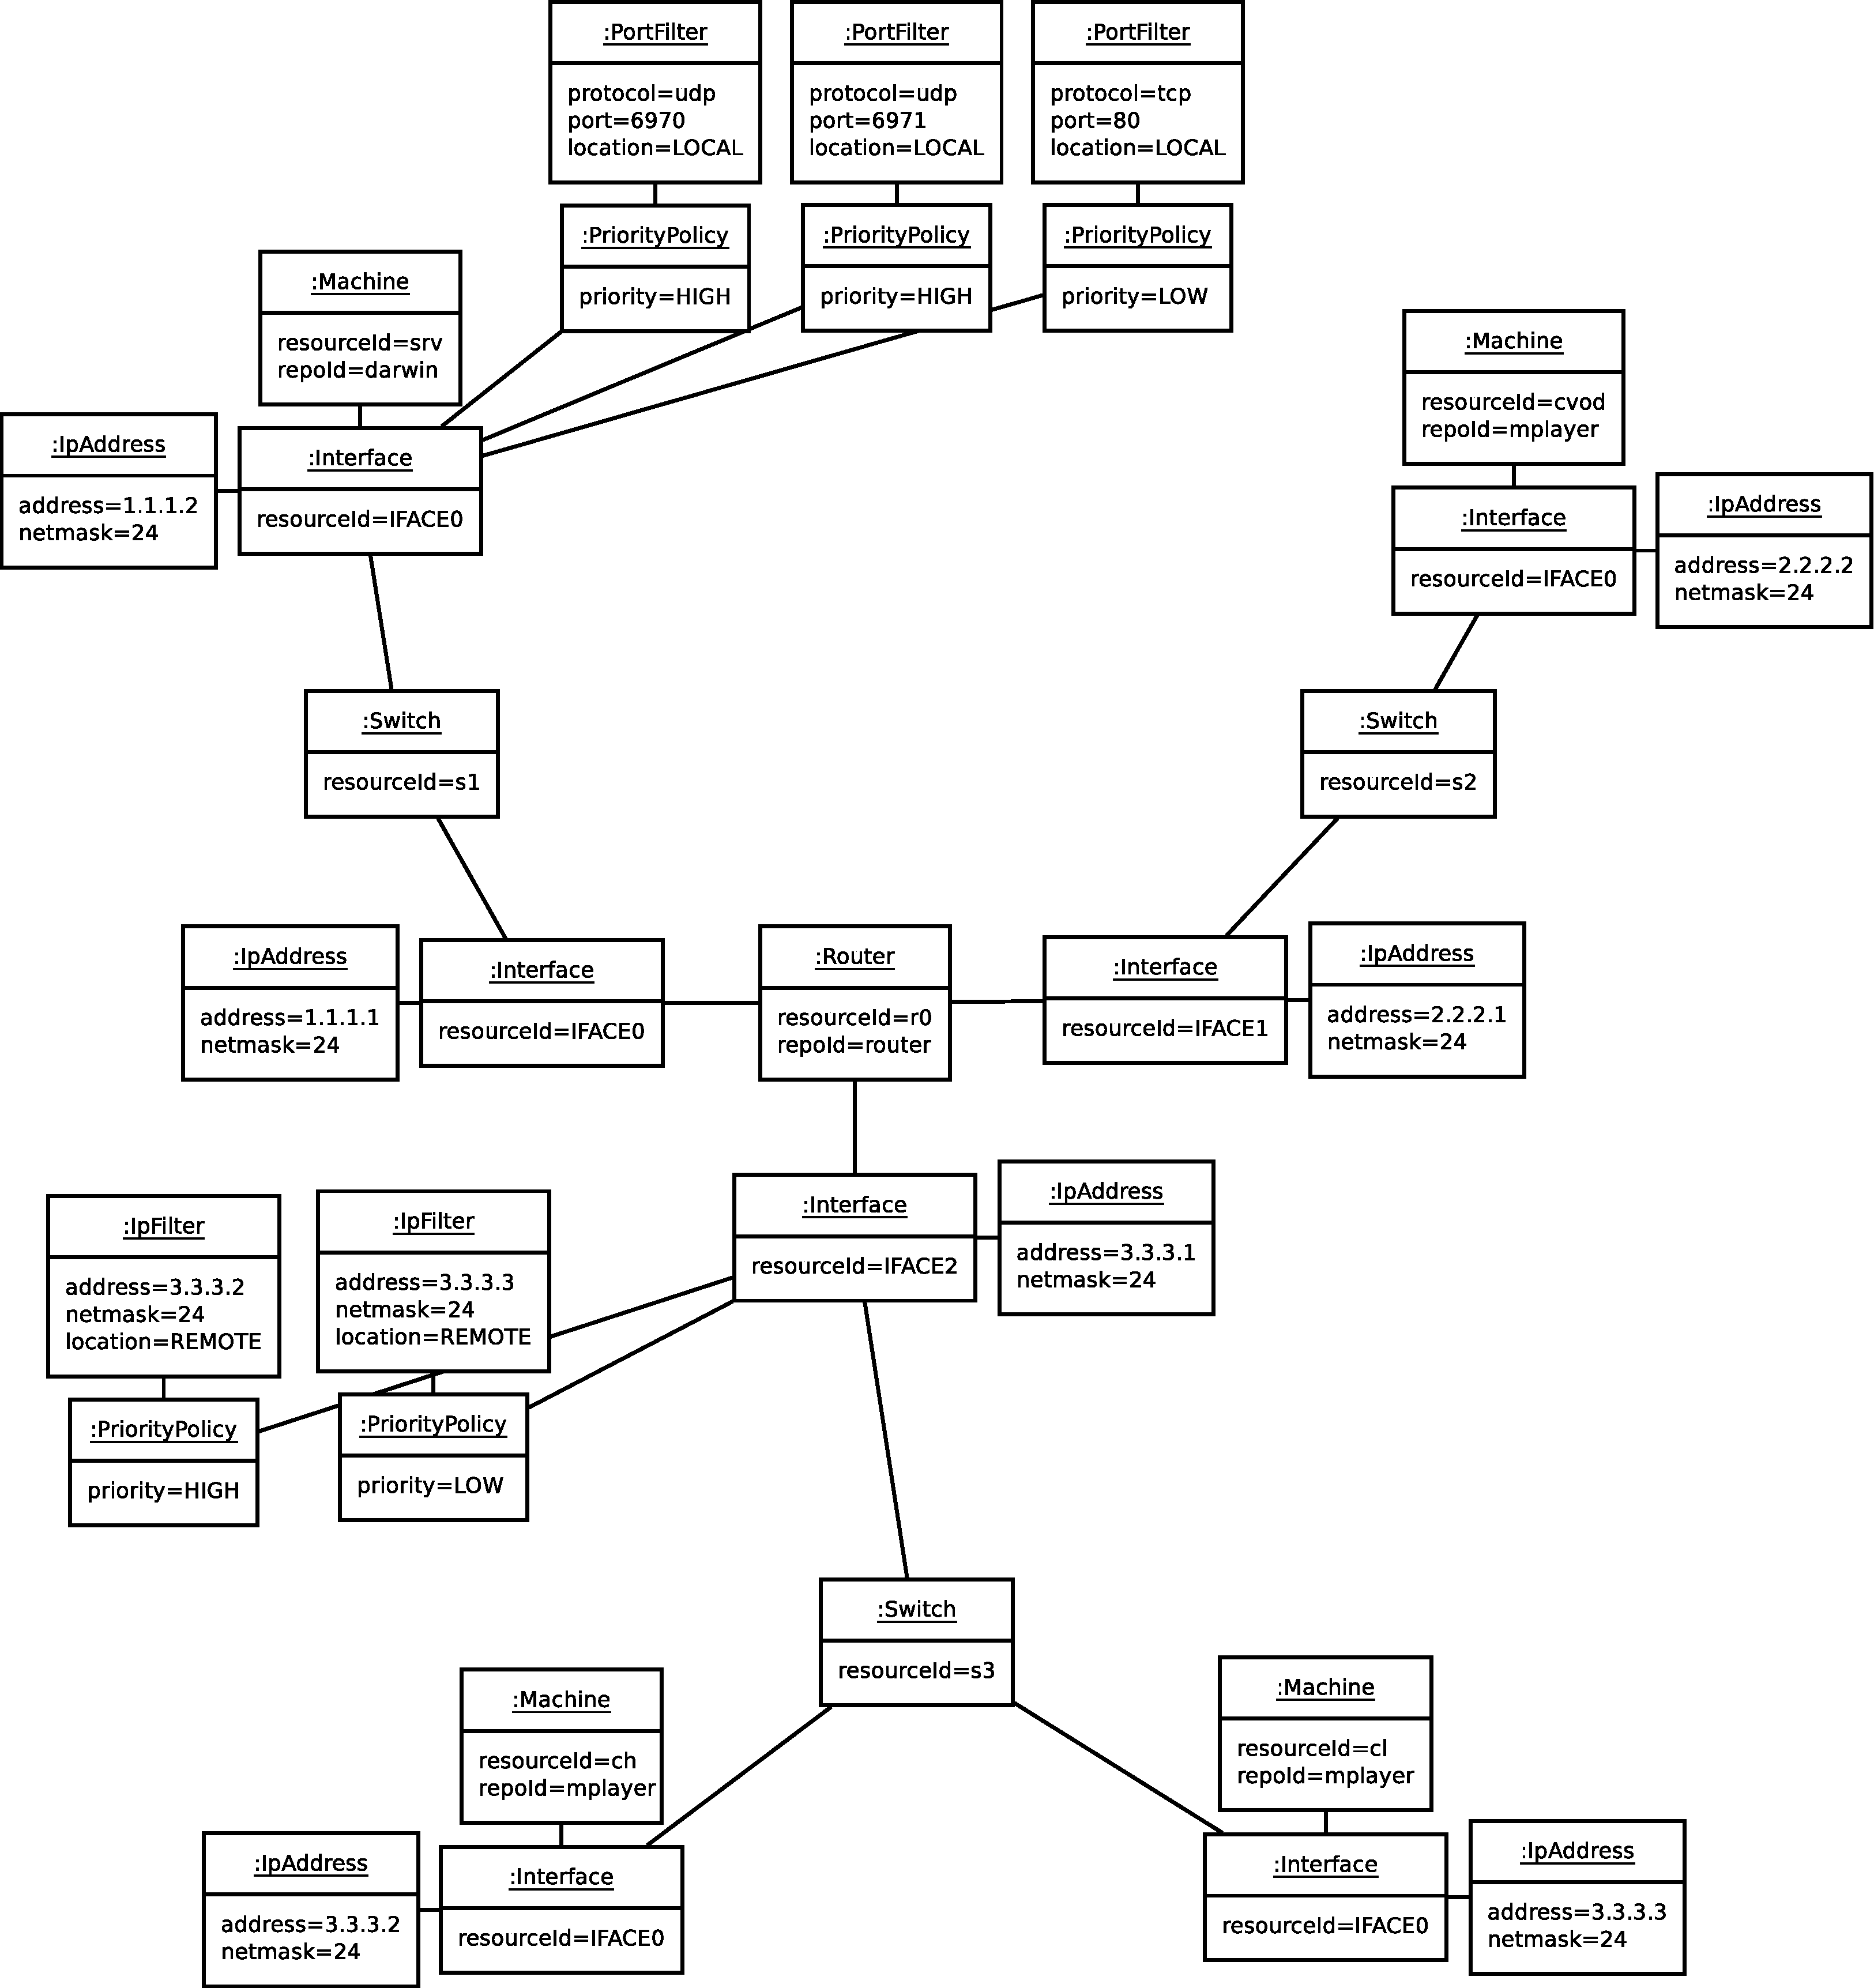
\includegraphics[width=.9\textwidth]{img/test-case/topology-om.pdf}

          \caption{Network topology expressed in terms of the domain model}
          \label{fig:cs:topo}
        \end{figure}

        % TODO ^ maxbw! pokolorowac?
      
      
      \subsection{Resulting Crossbow and Solaris components}
      \label{sub:uc:xbow}

        A successful model instantiation creates a number of Crossbow and Solaris entities. The resulting set contains
        zones, etherstubs, VNICs and flows that reflect the desired configuration. These entities work together and
        provide fully operational network topology.

        All the entity names follow the same pattern --- they are prepended with project identifier (\texttt{uc\_}).
        There are five zones created, as shown in listing \ref{lst:uc:xbow:zone} (one media server, three clients and
        one router). \\

        \noindent
        \begin{minipage}{\textwidth}
          \lstinputlisting[caption={All the zones created after model instantiation},label={lst:uc:xbow:zone}]{lst/uc-zone.sh}
        \end{minipage}

        Each of the zones has virtual interfaces (VNICs) assigned. Flows are created for some of the interfaces. The
        server zone and all of the client zones are connected to the router zone with etherstubs. Listing
        \ref{lst:uc:xbow:ether} enumerates the etherstubs, VNICs and flows are shown in listing \ref{lst:uc:xbow:vnic} \\

        \noindent
        \begin{minipage}{\textwidth}
          \lstinputlisting[caption={Etherstubs},label={lst:uc:xbow:ether}]{lst/uc-ether.sh}
        \end{minipage}

        \noindent
        \begin{minipage}{\textwidth}
          \lstinputlisting[caption={Virtual interfaces and flows created on top of them},label={lst:uc:xbow:vnic}]{lst/uc-vnic.sh}
        \end{minipage}


      \subsection{Media preparation}
      \label{sub:}

        For a movie to be streamed, hint tracks have to be created. Hints are meta-data that provide information on how
        to stream audio and video tracks. This information is then used by the server when dividing the media into
        packets and sending them via the network.

        The sequence of commands in listing \ref{lst:uc:media:prep} demonstrates how to prepare a movie to be streamed
        by Darwin Streaming Server (the example leverages ffmpeg\footnote{available at \url{http://www.ffmpeg.org}} and
        mpeg4ip\footnote{available at \url{http://mpeg4ip.sourceforge.net}} utilities). First, the data streams are
        transcoded to MPEG4 (video) and AAC (audio) formats and saved in an MPEG4 container. Then, hint tracks are
        appended to the container. \\

        \noindent
        \begin{minipage}{\textwidth}
          \lstinputlisting[caption={Media preparation before streaming},label={lst:uc:media:prep}]{lst/uc-prep.sh}
        \end{minipage}


    \section{The infrastructure operation}
    \label{sec:uc:operation}

      The traffic data is gathered as follows: each host node has tshark utility installed. It is set up to monitor all
      the traffic on the server interface and write it to a file (as shown in listing \ref{lst:uc:op:tshark}). When the
      gathering process is finished, the data is handed to wireshark and analyzed - graphs with throughput and jitter
      values are generated to show the interdependencies between the streams of data. \\

      \noindent
      \begin{minipage}{\textwidth}
        \lstinputlisting[caption={Monitoring network traffic with tshark},label={lst:uc:op:tshark}]{lst/uc-tshark.sh}
      \end{minipage}

      The tests include verifying that the set up bandwidth limitations work on per-client basis (TODO), different
      service types are treated according to the policy and streaming client differentiation requirements are satisfied.
      The main metric used is bandwidth each of the streams is assigned. Also, jitter is analyzed to estimate the
      Quality of Experience the user gets when watching streaming media (TODO).


      \subsection{Limiting the bandwidth}
      \label{sub:uc:limit}

        Bandwidth is limited to 8Mbps for all the links. The limits can be changed online with immediate effects. Figure
        \ref{fig:uc:limit} shows bandwidth limitation for a VOD client downloading a movie. After a short period of
        transmission rate limited to 24Mbps, the link bandwidth is narrowed to 8Mbps (lowest supported value).

        \begin{figure}[H]
          \begin{center}
            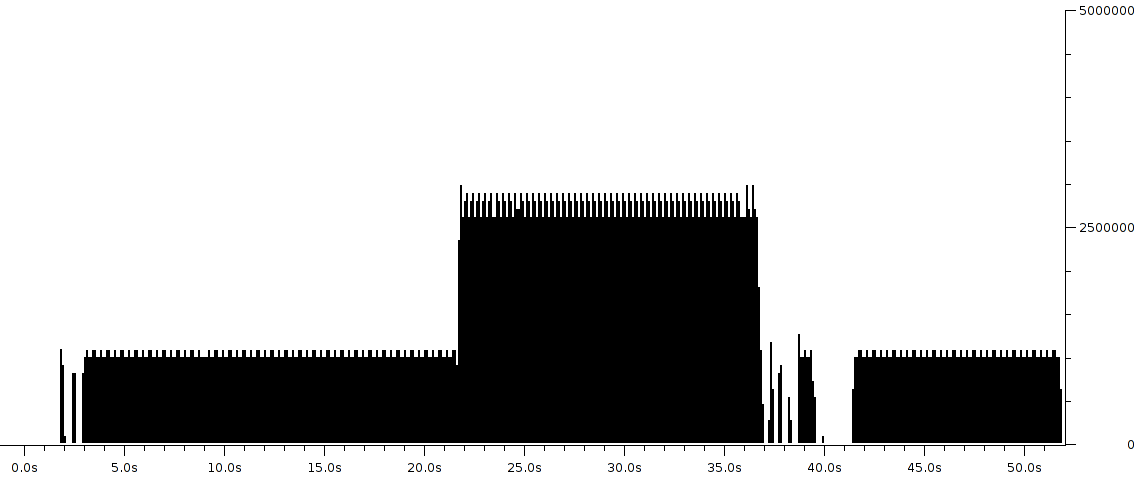
\includegraphics[width=.7\textwidth]{img/test-case/limit.png}
          \end{center}

          \caption{8Mbps bandwidth limitation}
          \label{fig:uc:limit}
        \end{figure}


      \subsection{Policies for different types of traffic}
      \label{sub:uc:traffic}

        A VOD client is downloading a long movie. All the bandwidth is available. Another client connects to the
        streaming server and requests a number of video streams. As the RTP data is of high priority, the streaming
        client is favoured over VOD client and it gets most of the available bandwidth.

        \begin{figure}[H]
          \begin{center}
            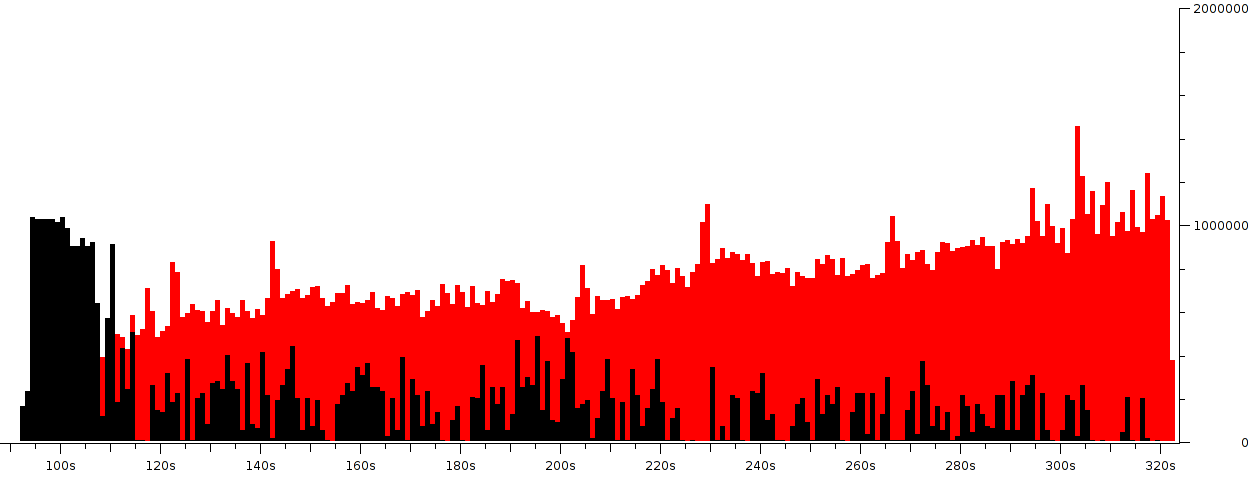
\includegraphics[width=.7\textwidth]{img/test-case/vod-rtp.png}
          \end{center}

          \caption{VOD traffic bandwidth consumption compared to high-priority RTP streams}
        \end{figure}


      \subsection{Client-dependent quality of service}
      \label{sub:uc:client}

        A VOD client is downloading a movie. Two clients connect to the streaming server and request a number of video
        streams. One of the streaming clients has low priority assigned, the other one is high priority. RTP streaming
        gets most of the bandwidth and high priority client is favoured over the low priority one.

        \begin{figure}[H]
          \begin{center}
            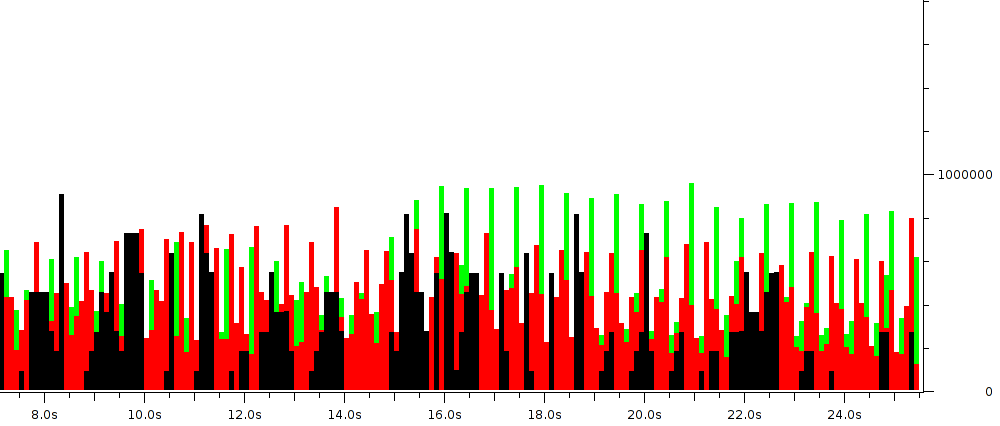
\includegraphics[width=.7\textwidth]{img/test-case/exp-all.png}
          \end{center}

          \caption{Distribution of available bandwidth between streaming clients}
        \end{figure}


    \section{Enhancements provided by the solution}
    \label{sec:uc:enhance}

      The implemented system provides extensive support for most of the stages that comprise virtual network management.
      There are two main goals the system is designed to achieve: to limit the time spent by the administrator to create
      and manage the topology and to make the process as intuitive as possible.


      \subsection{Topology design}
      \label{sub:uc:enhance:design}

        The GUI console displays the topology in the form of a graph --- with virtual appliances (or switches) as nodes
        and connections as edges. With the approach it is easy to visualize the structure of the network so that it can
        be quickly understood and adjusted.

        All the essential aspects of the network design are configurable with GUI wizards. The system provides an easy
        way to set up addressing, routing and quality policies. Also, appliance repository access is integrated. Input
        data describing the model is validated while being entered by the user. 


      \subsection{Infrastructure instantiation}
      \label{sub:uc:enhance:instantiation}

        By automating the instantiation process (ie. snapshot retrieval and transfer, zone attachment and configuration)
        a lot of user's time is saved. This does not only cover the time required to log in to a host system and enter
        commands manually --- the instantiation stages, when possible, are performed concurrently and can save
        significant amount of time required by this process.

        Input validation minimizes the risk of mistakes, especially when big topologies are considered and the whole
        design becomes complicated. A consistent naming scheme is provided so that the topology can be managed when the
        system is not available.

        % TODO progress bar, czy tutaj, czy w implementacji?
        % TODO nawiazanie do deploymentu z va (chapter: solaris)


      \subsection{Online modifications}
      \label{sub:uc:enhance:online}

        With online modification support it is easy to adjust the system without breaking its operation. The quality
        policies, for example, already instantiated can be changed, whenever needed.

        Even more sophisticated control is possible. For example, additional rule-based component could be developed and
        integrated with the system to allow automatic adjustment based on statistical data.


      \subsection{Monitoring}
      \label{sub:uc:enhance:monitoring}

        Historical data can be accessed. There are customizable usage charts that can display bandwidth usage for
        policies and interfaces. Also, load on the host machine can be monitored to help designer assess which machines
        to choose when assigning the appliances.


    \section*{Summary}

      The chapter presented all the steps that were undertaken to ensure the system meets the identified requirements.
      The ability to create and manage complex network topologies was demonstrated by designing and instantiating
      multimedia oriented network with wide variety of components used. Validity and operation of deployed
      infrastructure was confirmed by the tests performed. It was shown that communication between virtual appliances is
      possible with properly configured routing tables. And, most importantly, the experiments confirmed that Quality of
      Service policies are preserved.


  \chapter{Summary}

    \section*{Chapter overview}

	  This chapter summarizes the outcome of research in the area of network virtualization with special regard to 
	  Solaris and the Crossbow package and its functionalities. 
	  
	  Section \ref{sub:sum:concl} briefly concludes research results and test-case results.
	  Section \ref{sub:sum:achieved} outlines realized goals.
	  Section \ref{sub:sum:further} considers possible improvments that might be introduced to created system.

    \section{Conclusions}
		\label{sub:sum:concl}
		
		Deep investigation during work on this paper allowed better understanding concepts like network virtualization,
		resource reservation. Preformed tests additionally outlined the significance of these issues and how important they
		are in terms of success of developed system. Encountered complex problems only confirmed that although very useful 
		they are also quite demanding and require comprehensive knowledge in all computer areas.
		
    \section{Achieved goals}
		\label{sub:sum:achieved}
		
		In terms of achieved goals not all were successfully finished. Time shortage and lack of people did not allow 
		for as deep insight look at this issue as was initially planned. However, some objectives are really worth to
		be mentioned:
	  
		\begin{itemize}
			\item{Significant improvement in system configuration in comparision to manual configurating,}
			\item{Presenting network in clear way ( graph format ).}
		\end{itemize}
		
	    Hopefully presented system and whole concept of network virtualization, resource allocation and isolation 
	    would encourage reader to do own research in this area.
		
		

    \section{Further work}
		\label{sub:sum:further}
	
      In terms of the future work there are many improvements that might be implemented. Probably the largest component,
      which was initially plannned, was automatic resource assigner, that would run and perform automatic resource
      assignments to nodes that run under lowest load. This assigner with attached rule based system would gather data
      about the load on each node and based on that decide what and where instantiate. Presented and discussed system in
      this thesis lacks that functionality. Instead, it offers manual assignments, where user selects on which node new
      virtual resources should be created. Another not implemented yet welcomed would be semi-automatic snapshot creation. 
      Currently user can create solaris zone from existing snaphot and use it. Functionality where created resource could be 
      converted to snapshot and then transfered to the repository would definately improve the usability of the system.


  \bibliographystyle{plain}
  \bibliography{bibliography}


\end{document}

% vim: et : tw=120 : spelllang=en_us,pl : spell :
